\chapter{焦点面検出器アライメントの較正}
\label{chapter4}

GroundBIRD実験での偏光測定のためには、検出器間での信号の差分を取ることが重要であり、それに伴って望遠鏡のスキャンに対して最適な検出器のアライメントが求められる。この章では検出器アライメントの最適化に向けた改善を行い、観測データからその効果を確認した。

\section{検出器アライメントの問題点}

\subsection{スキャン軸に対する傾きと差分解析}
\label{scan_pair_diff}
まず、GroundBIRDでの解析手法の1つである差分解析と検出器アライメントの関係について述べる。\ref{mkid_design}で示したように、焦点面検出器は異なる偏光方向に感度を持った検出器が交互に配置されている。これらの検出器が検出する信号は空のある点からの放射が望遠鏡内の光学系を経て焦点面へと届いたものである。つまり、焦点面での検出器の配置を空へと射影した時にどう配置されているかが重要になる。各検出器は空のある点を見ており、望遠鏡の方位角回転に伴って同じ仰角の空を回転しながら観測する(図\ref{scan_image})。
\begin{figure}[htbp]
  \centering
  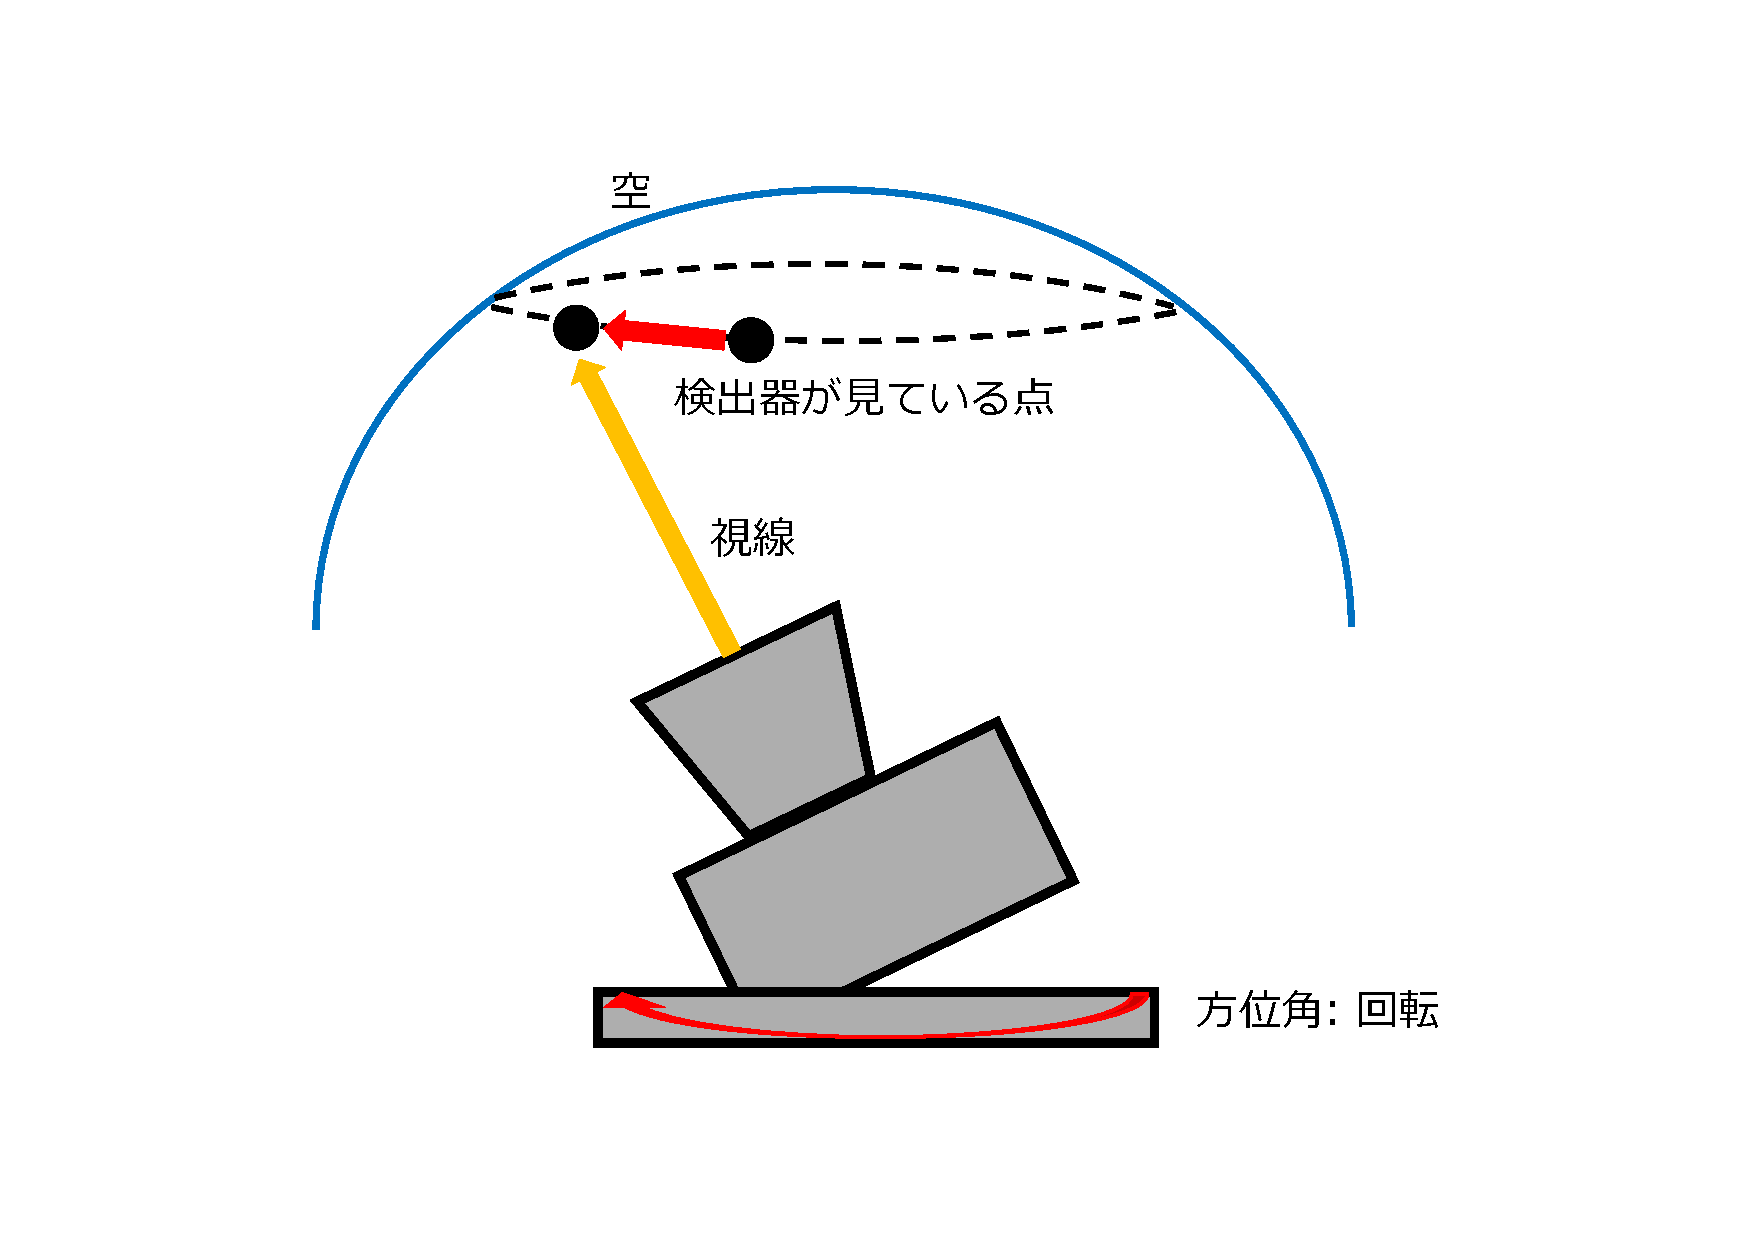
\includegraphics[width=0.6\columnwidth]{5_alignment/figs/scan_image.pdf}
  \caption{検出器が空の領域をスキャンする概要図。ある仰角を高速回転しながらスキャンする。}
  \label{scan_image}
\end{figure}
検出器で観測する信号は大きく(CMB + ノイズ)に分けられる。さらにノイズの中でも寄与が大きい成分に大気放射に由来するノイズがある。このノイズは刻一刻と変動する上に空の領域によっても異なっているため、高速回転によるスキャンで異なる検出器が同じ空の領域をスキャンすることで抑制できる。具体的には、異なる偏光方向に感度のある検出器が同じ仰角の空をスキャンする時、もう一方の検出器は片方の検出器が観測した空の領域をわずかな時間差で観測することができる。つまり、スキャンの間に大気の情報は変動せず観測される大気由来のノイズも変動しないことになる。そのため、検出器間で信号の差分をとることで、大気ノイズは共通していると考えれば取り除くことができ、偏光成分のみを残すことができる。しかし、検出器の配置がずれていて検出器間でスキャンする空の領域が異なる場合、大気の情報も異なり、差分をとっても大気ノイズを取り除くことができない(図\ref{scan_axis})。
\begin{figure}[htbp]
  \centering
  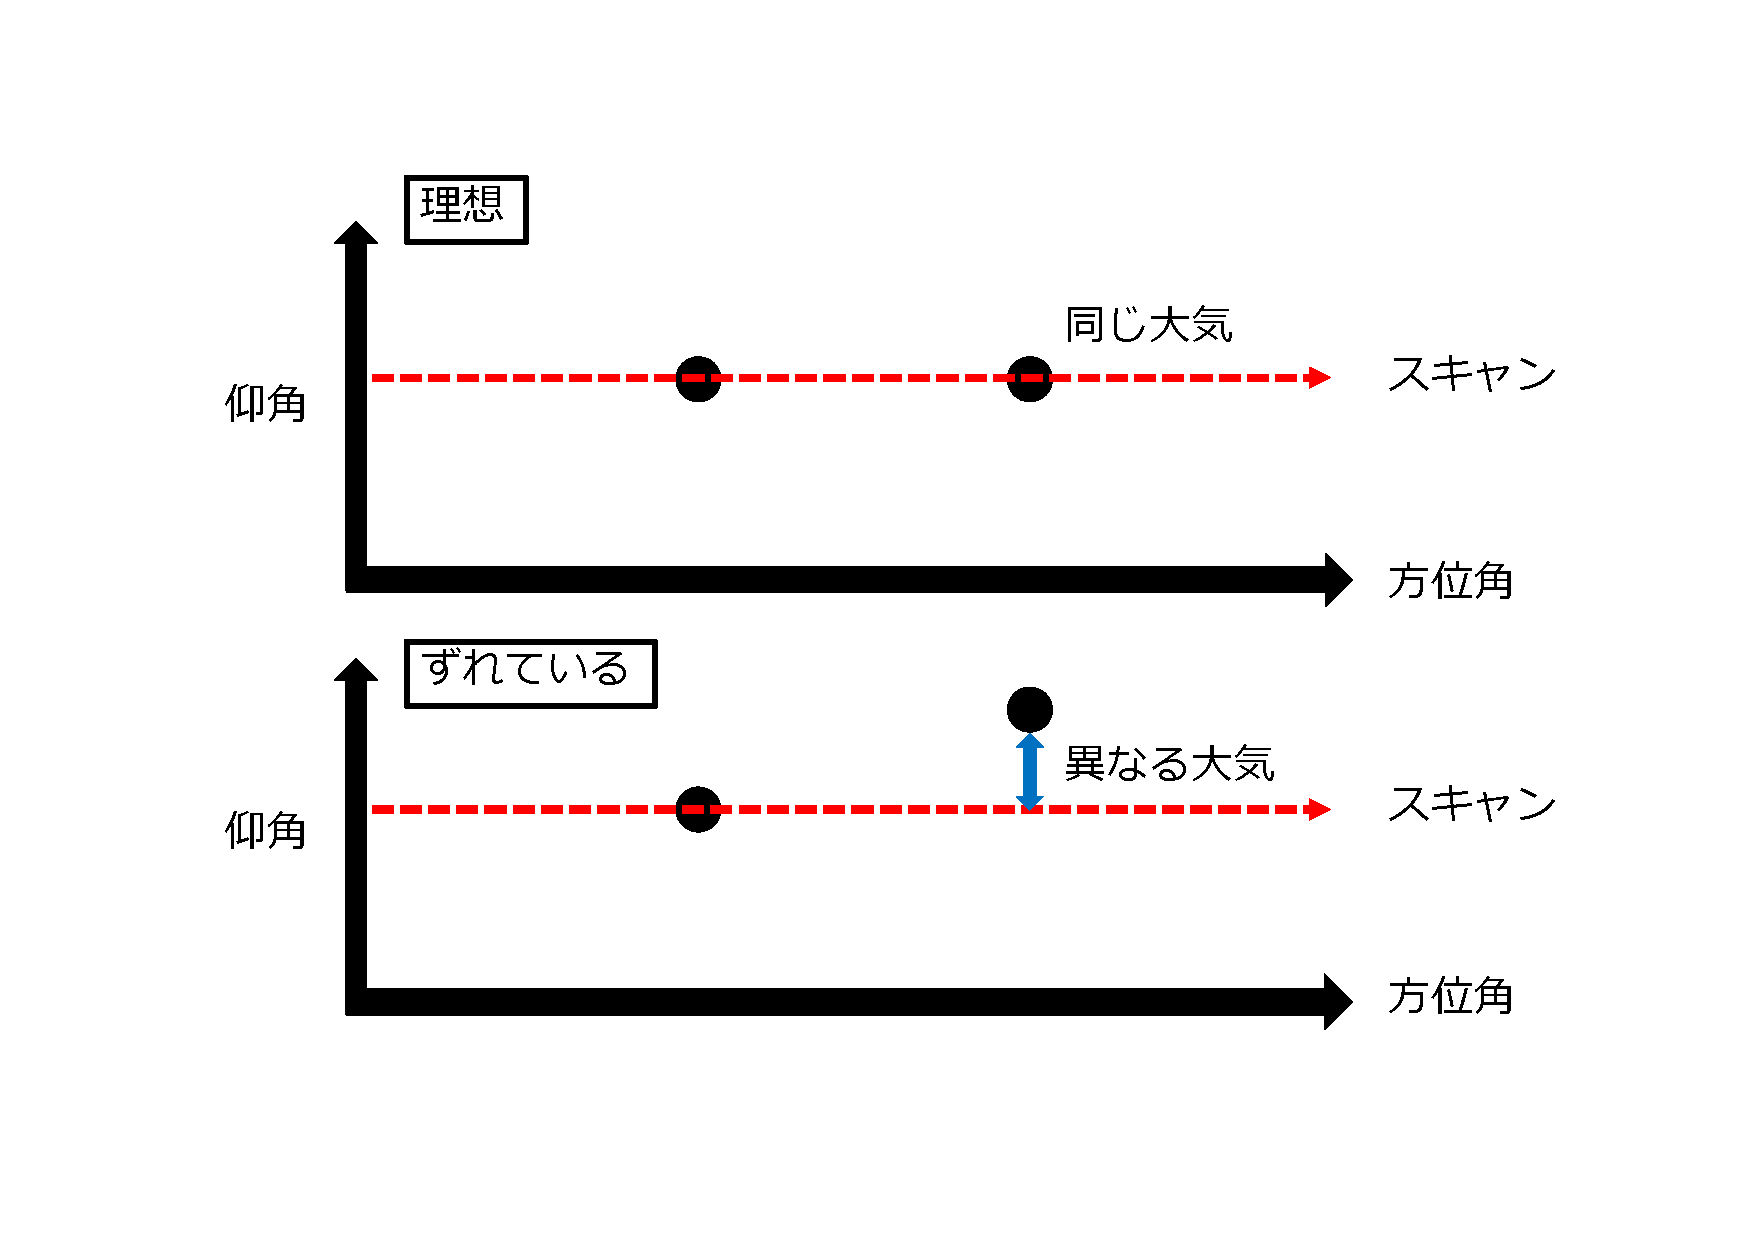
\includegraphics[width=0.7\columnwidth]{5_alignment/figs/scan_axis.pdf}
  \caption{空での理想的な検出器の配置とずれている場合の配置との比較。スキャン軸(方位角軸)に沿って検出器が並んでいないと観測する大気が検出器ごとに異なる。}
  \label{scan_axis}
\end{figure}

以上から空での理想的な検出器の配置は``複数の検出器がスキャン軸に沿って並んでいる''ことである。

しかし、観測データから理想的な検出器の配置からずれていることが示唆されていた。また、そのずれはスキャン軸に対して無視できないほどに有意な角度で傾いているものだと考えられていたが十分な検証と較正(実際に何度傾いているのか、傾きがあることでどれ程大気ノイズの影響が残ってしまうのか、など)がされていなかった。検出器アライメントの問題を改善し、GroundBIRDが持つ観測性能を最大限に引き出すことは質の良いデータを取得するためには不可欠である。

\subsection{要求される理想的なアライメント}

GroundBIRDにおける理想的な検出器の配置について詳細を見ていく。焦点面検出器は図\ref{full_array_picture}のように7つの検出器アレイが平面的に取り付けられているが、この検出器が観測する領域は平面のまま空に射影される訳ではない。観測する空の点は天球面上に張り付いた点と考えられるため、球面として射影される。焦点面検出器が平面を見るときと空を見る時での理想的な配置の違いを図\ref{distortion_pos}に示す。実際には球面から来る歪みの影響を受けた配置として空を観測することになり、望遠鏡の視線中心(\SI{220}{GHz}アレイ)ではほぼ平面だが、中心から離れた検出器は歪みの影響が出る。歪みを考慮した上で複数の検出器をスキャン軸に沿って並べることは焦点面の設計上難しい。また、高周波になるほど大気放射の寄与が大きくなる\cite{atmos_radiation}ことから、本論文では歪みの影響が少なく、大気放射の寄与も大きい中心の\SI{220}{GHz}アレイに対して配置がスキャン軸に沿って並んでいること、中心以外の\SI{145}{GHz}アレイに対して配置が仰角軸に対称であることを理想的なアライメントとする。
\begin{figure}[htbp]
  \centering
  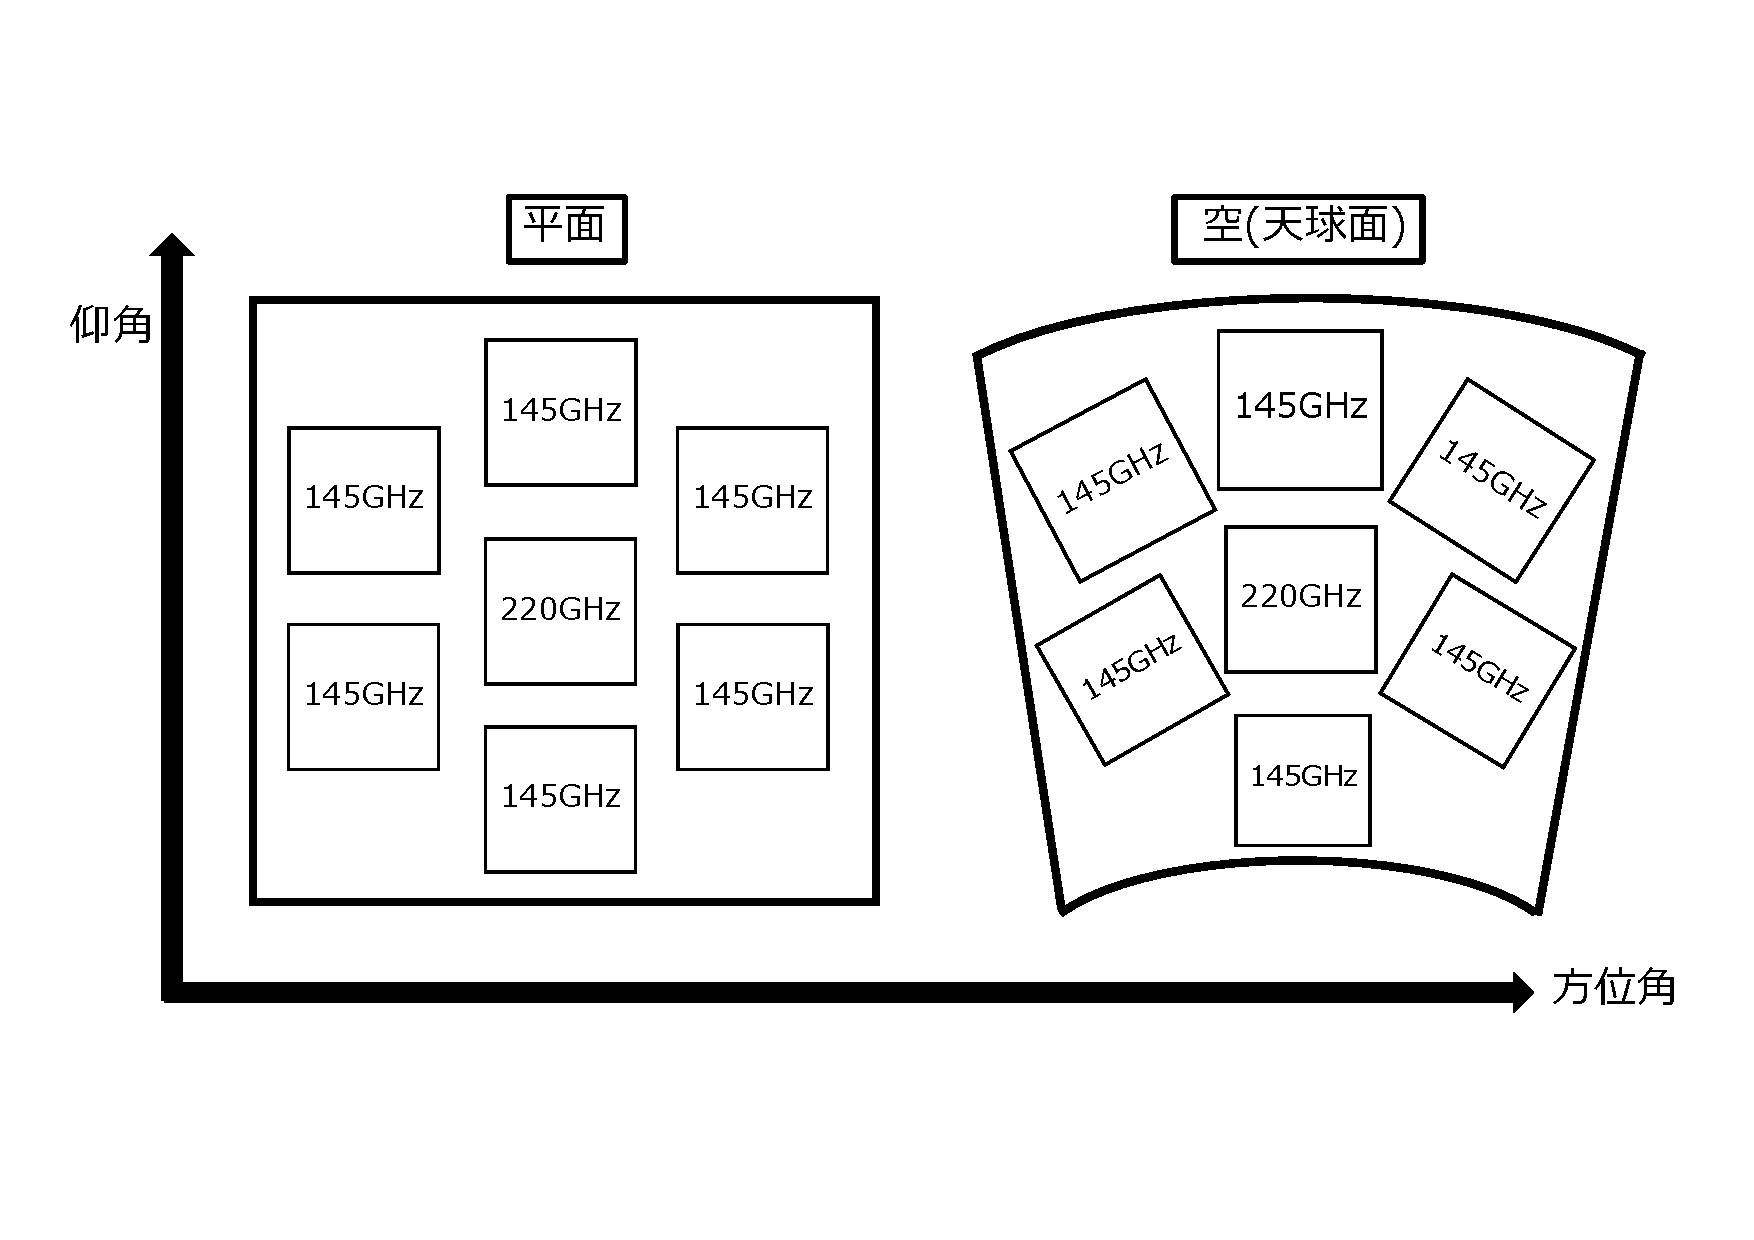
\includegraphics[width=0.8\columnwidth]{5_alignment/figs/distortion_pos2.pdf}
  \caption{平面と空(天球面)での理想的な検出器配置の違い。}
  \label{distortion_pos}
\end{figure}
\subsection{視線軸方向まわりの回転による較正}

スキャン軸に対して傾いた焦点面検出器を理想とする配置にするためには、検出器の視線を回転させてスキャン軸に並べれば良いことになる。また、焦点面検出器は望遠鏡内部で固定されているため望遠鏡全体の視線を回転することに対応する。つまり、望遠鏡のビーム中心を望遠鏡の視線方向とし、視線方向軸周りに適当な角度回転させることで各検出器の視線を回転させる(図\ref{boresight_axis})。
\begin{figure}[htbp]
  \centering
  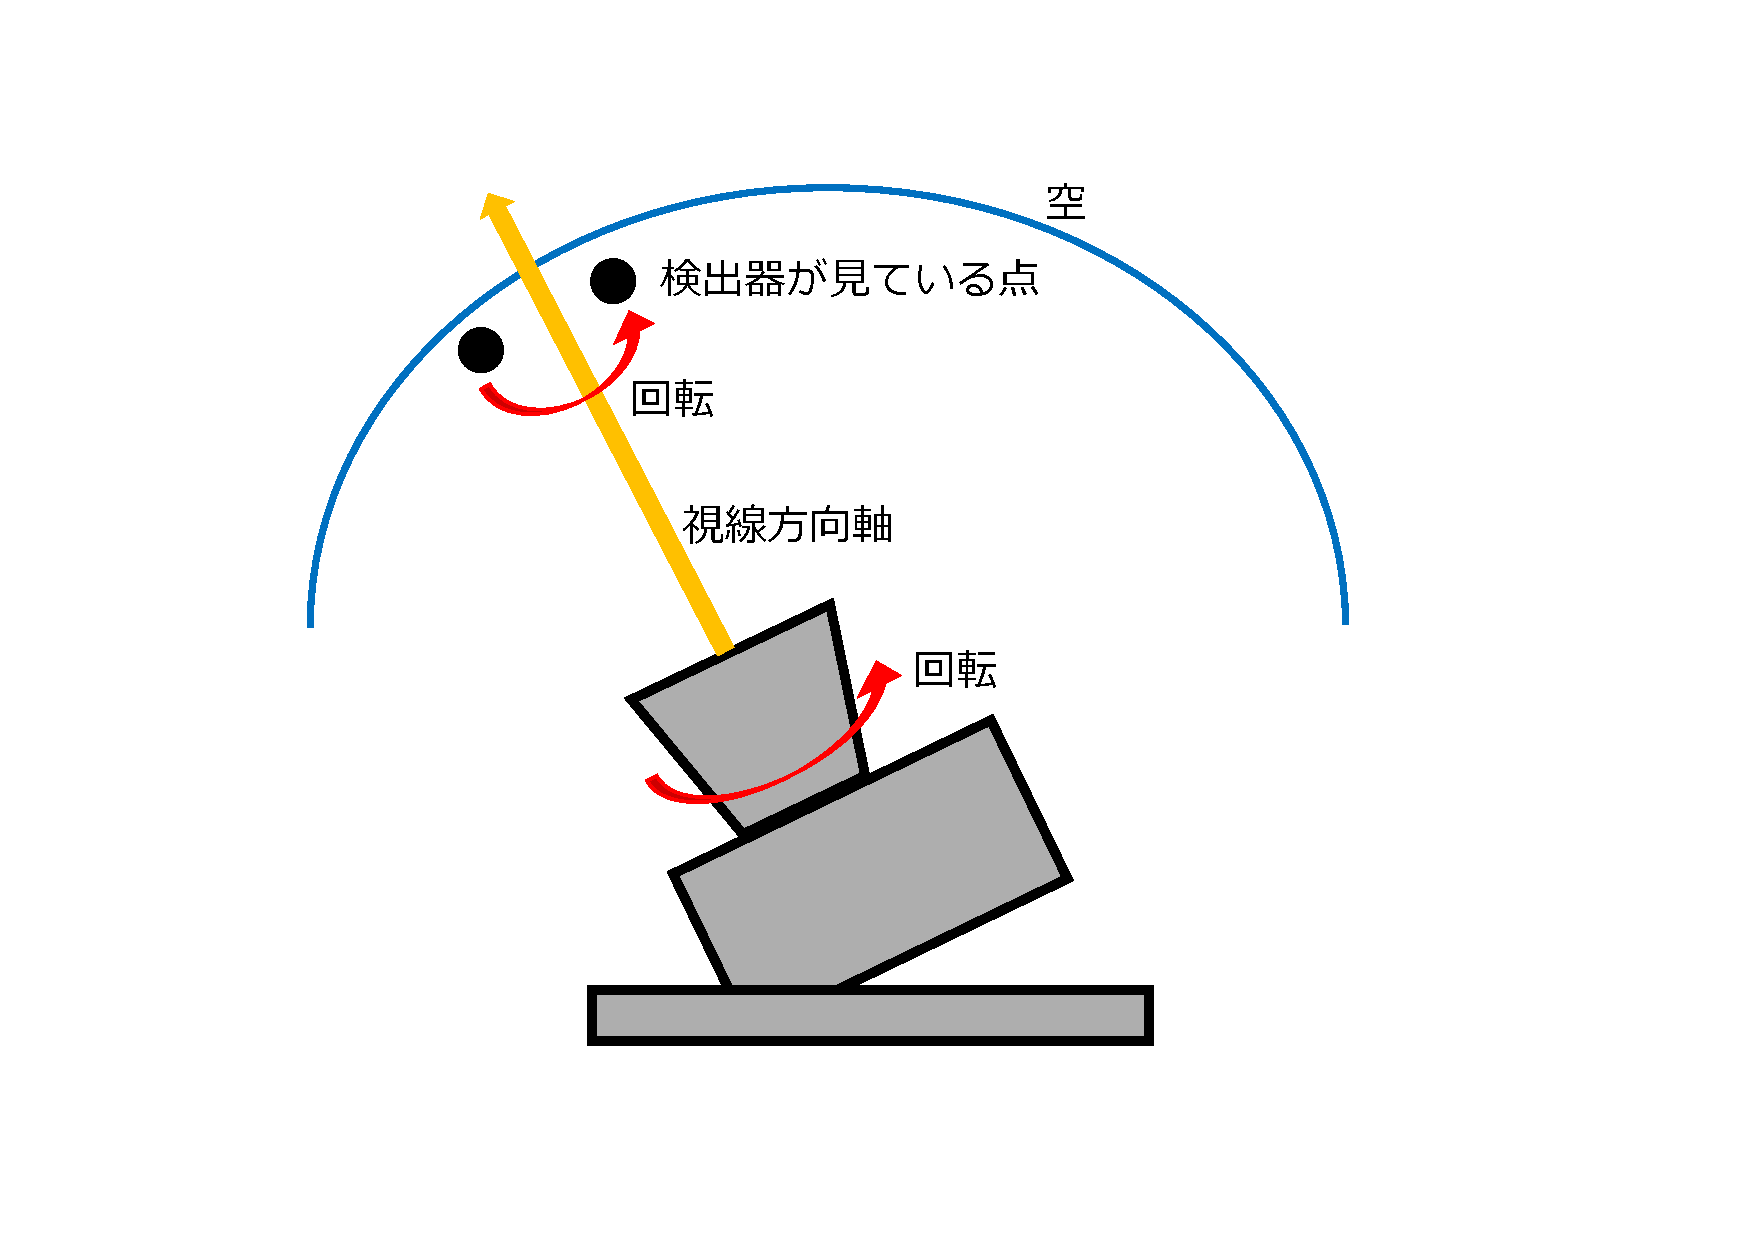
\includegraphics[width=0.8\columnwidth]{5_alignment/figs/boresight_axis.pdf}
  \caption{望遠鏡の視線方向軸と軸周りの回転。検出器の見ている点(視線)も回転する。}
  \label{boresight_axis}
\end{figure}
%検出器の配置がビームの中心に対して傾いている場合、視線方向軸の周りに望遠鏡を適当な角度回転させることで配置をスキャン軸に沿って並ばせることが可能になる。

そのため、理想的なアライメントにするための回転角を見積もる必要がある。回転角を求めるには各検出器の見ている点を知る必要があり、天体の観測データを解析することで算出できる(天体の運動が分かっているので検出器データと角度データから各検出器の視線情報を求められる)。

\section{月を用いた回転角の算出}

\subsection{月を用いた理由}

GroundBIRDで観測できる天体として月や惑星(木星、金星)が挙げられる。しかし、月と惑星ではデータの性質は大きく異なり、それぞれ観測上の長所と短所が存在する。月データと惑星データの特徴を表\ref{moon_vs_planet}に示す。
\begin{table}[htbp]
%\begin{threeparttable}[htbp]
  \centering
  \caption{月データと惑星データの比較\cite{sueno_doctor}}
  \vspace{3mm}
  \begin{tabular}{ccc} \hline
    & 月 & 惑星 \\ \hline
    長所 &
    \begin{tabular}{c}
    S/N比が高い \\ (1度の観測で十分な信号を得られる)
    \end{tabular} &
    \begin{tabular}{c}
    点源として扱える \\ (角直径がビーム幅に比べて十分小さい)
    \end{tabular} \\ \hline
    短所 &
    \begin{tabular}{c}
    点源として扱えない \\ (輝度温度の非一様性が生じる)
    \end{tabular} &
    \begin{tabular}{c}
    S/N比が小さい \\ (データを蓄積しないとノイズに埋もれる)
    \end{tabular} \\ \hline
  \end{tabular}
  \label{moon_vs_planet}
\end{table}
%\end{threeparttable}
検出器の視線情報を得るには点源として扱え、正確に点として求められる惑星が適しているが、\ref{jupiter_ana}で見るように点源で最も明るい木星の観測データでもノイズの影響をかなり受けてしまう。そのため、データを蓄積するか、PWVや湿度が十分低く観測条件が整った観測データを使用する必要がある。一方、月は高いS/N比により1度の観測データで十分な信号を得られ、データを蓄積することによるノイズが加わることなく解析ができる。点源として扱えないことによる誤差はあるものの\footnote{月の輝度温度は月齢によって大きく変動し、月齢を$\phi$~[deg]、波長$\lambda$に対して$\delta=0.3\cdot\lambda$~[mm]とすると、輝度温度$\overline{T_{\mathrm{MOON}}}$は
\begin{equation}
  \overline{T_{\mathrm{MOON}}}=225\Bigl\{1+\frac{0.77}{\sqrt{1+2\delta+2\delta^{2}}}\cos\bigl(\phi-\arctan\frac{\delta}{1+\delta}\bigr)\Bigr\}
\end{equation}
と経験的に表せる\cite{dennpa_tennmonn}。}、高いS/N比がそれをカバーできると考えたため、月のデータを選択した。

\subsection{位相としての検出器TOD}
GroundBIRDにおける観測データは\ref{MKID}で述べた超伝導検出器MKIDの共振状態の変化を入射信号の大きさとして\SI{1}{kSPS}で取得するTODのことである。共振状態の変化とはすなわち共振周波数の変化であるが、これを読み出しRF信号の透過率の変化として測定する。透過率は散乱行列要素の$S_{21}$で表す。MKIDの$S_{21}$は共振の鋭さを表す$Q_{r}$, $Q_{c}$を用いて
\begin{equation}
  |S_{21}-x_{c}| = \frac{Q_{r}}{2Q_{c}} \bigl(x_{c} = 1-\frac{Q_{r}}{2Q_{c}}\bigr)
\end{equation}
で得られ\cite{muto}、$S_{21}$の軌跡が円状になることが分かる。この円は``共振円''と呼ばれる。共振円と$S_{21}$の例を図\ref{res_circ}に示す。
\begin{figure}[htbp]
  \centering
  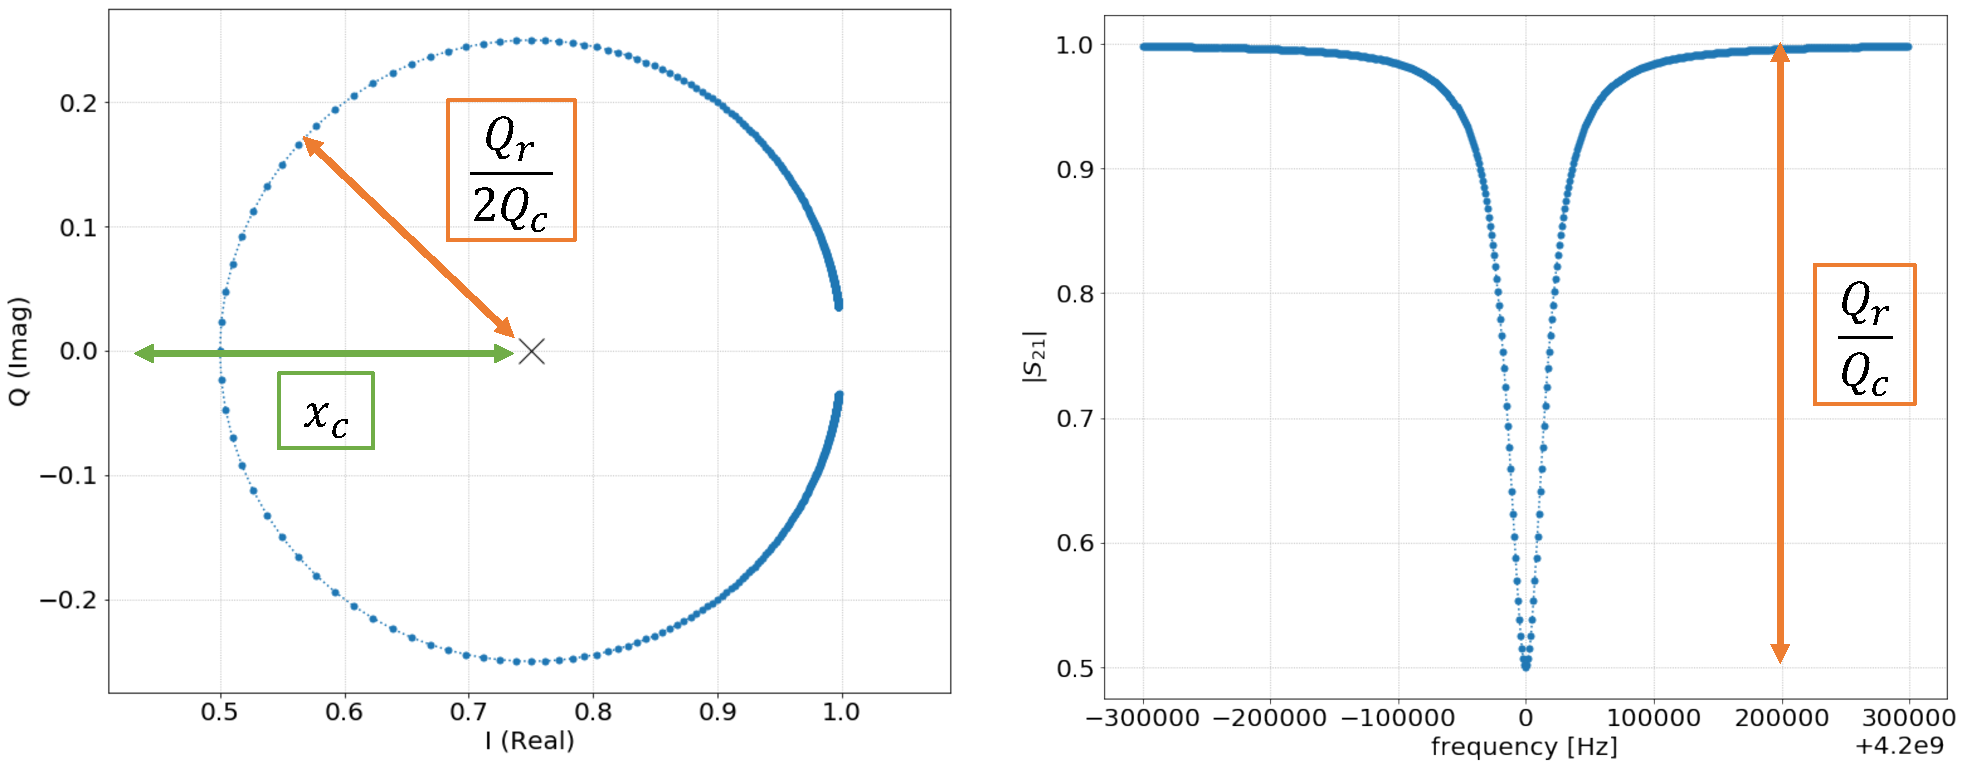
\includegraphics[width=1.0\columnwidth]{5_alignment/figs/iq_amp.pdf}
  \caption{共振円と共振周波数付近での透過率。\cite{sueno_master}より引用。}
  \label{res_circ}
\end{figure}
共振周波数の周りで透過率が鋭いピークを持つことが分かる。共振円を動く$S_{21}$の振幅$A$と位相$\theta$を
\begin{equation}
  A = \frac{|S_{21}|- x_{c}}{1-x_{c}}
\end{equation}
\begin{equation}
  \tan\theta = \frac{\mathrm{Im}(S_{21})}{x_{c}- \mathrm{Re}(S_{21})}
\end{equation}
と定義する。これらの値は共振周波数の変化に対して敏感であるため、振幅の変化($\delta A$)と位相の変化($\delta\theta$)によって入射信号の大きさを読み出せる。入射信号によって振幅と位相が変化する例を図\ref{amp_and_phase}に示す。
\begin{figure}[htbp]
  \centering
  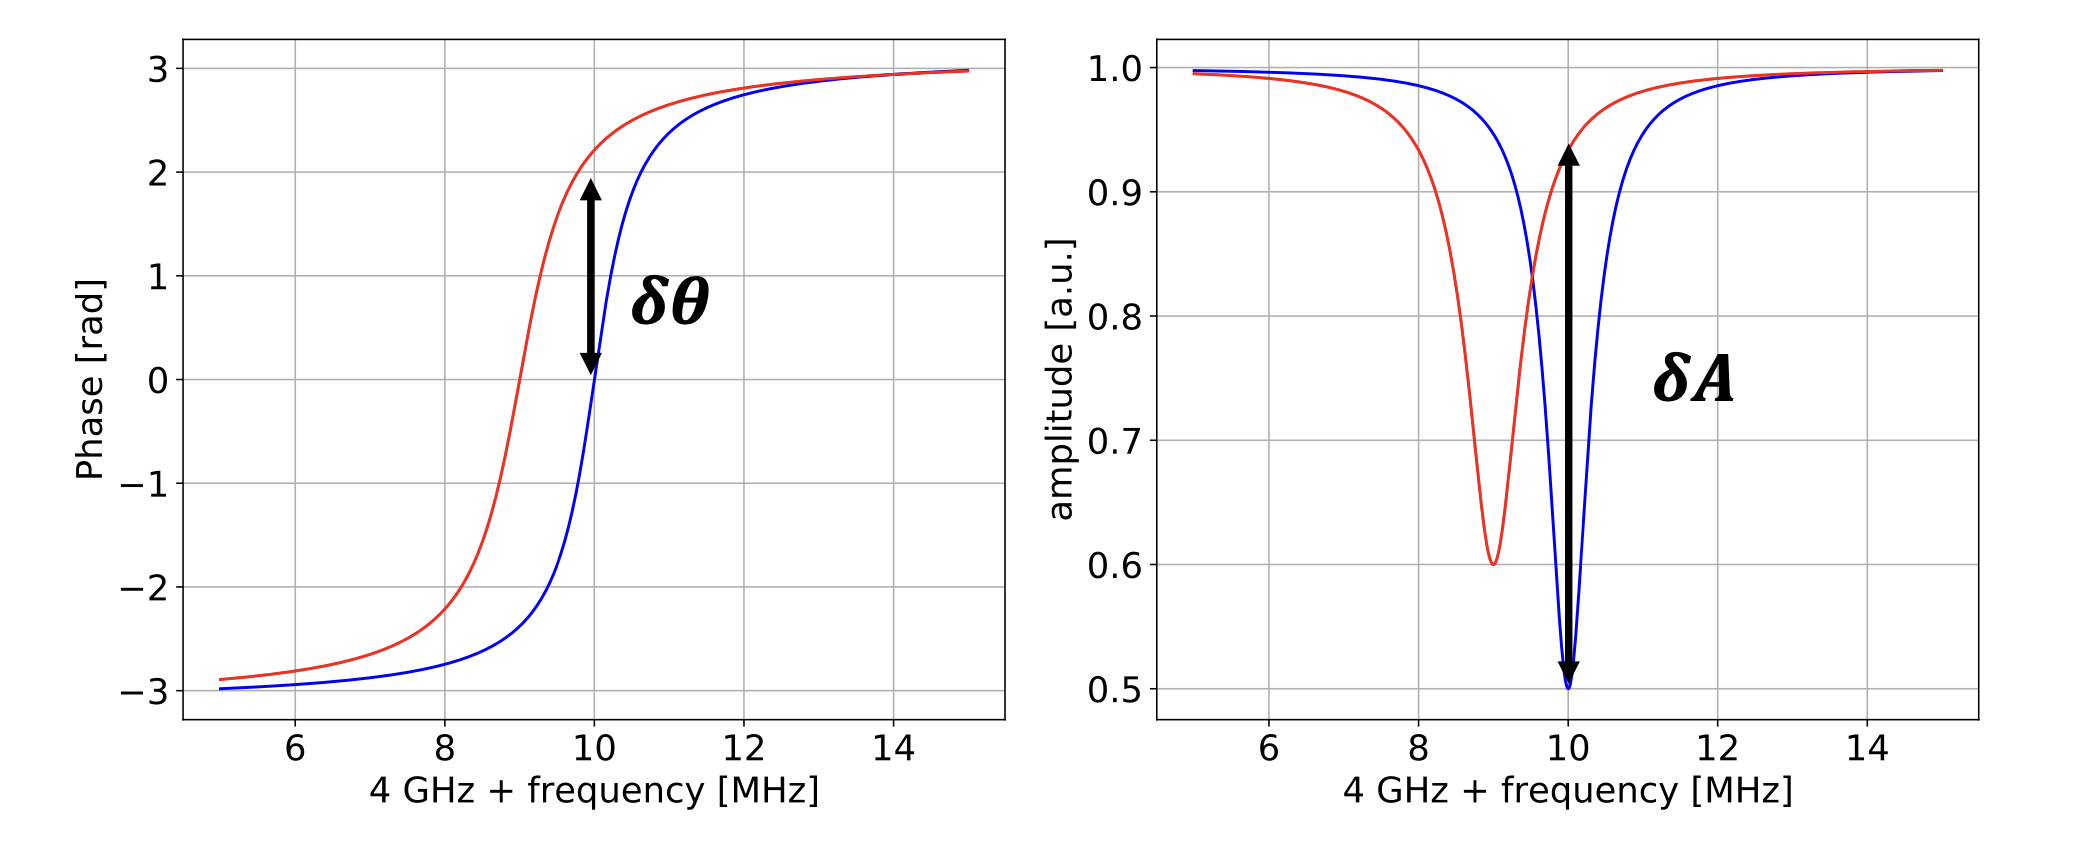
\includegraphics[width=1.0\columnwidth]{5_alignment/figs/amp_and_phase.png}
  \caption{共振周波数付近での$S_{21}$の振幅と位相の変化。\cite{sueno_doctor}より引用。}
  \label{amp_and_phase}
\end{figure}

実際のTOD取得時には図\ref{amp_and_phase}のように各MKIDで固定した共振周波数で測定を行う。そのため、TOD取得前に各MKIDの共振周波数を知る必要がある。また、共振周波数は観測条件によって変動するため、一定の値をとらない。そのため、1観測を1時間で区切っており、1観測ごとにTOD取得前に共振周波数を求めている(その間も望遠鏡は連続的に稼働している)。共振周波数を知るために
\begin{enumerate}
  \item 周波数スイープ
  \item フィッティング
\end{enumerate}
の手順で測定をする。周波数スイープとは、読み出し用のRF信号の周波数を少しずつ変えながら測定をする手法である。測定量はRFの透過率で、スイープで測定されたデータを透過率の関数でフィットすることで共振周波数を求める。フィット関数は$S_{21}$に補正項を入れたもので
\begin{equation}
  T_{21}(f) = a_{0}~\mathrm{exp}(-2\pi if\tau_{0})\biggl(1-\frac{Q_{r}/Q_{c}e^{i\phi}}{1+2iQ_{r}(f-f_{r})/f_{r}}\biggr)
\end{equation}
で表される\cite{sueno_master}。ここで、$a_{0}$, $\tau_{0}$は読み出し回路による振幅の減衰と位相のずれを表す。$e^{i\phi}$はCカップリングでのインピーダンスを補正する項である。このフィットで共振周波数$f_{r}$と共振の鋭さを表す$Q_{r}$, $Q_{c}$を得られる。得られた$f_{r}$にRF周波数を固定し、TODを取得する。TODでの測定量は$T_{21}$であり、補正項の効果を差し引くことで$S_{21}$としての振幅$A$と位相$\theta$を取得できる。
%\begin{equation}
  %|S_{21}-x_{c}| = \frac{Q_{r}}{2Q_{c}} \bigl(x_{c} = 1-\frac{Q_{r}}{2Q_{c}}\bigr)
%\end{equation}
%で得られ\cite{muto}、$S_{21}$の軌跡が円状になることが分かる。この円は``共振円''と呼ばれる。共振円と$S_{21}$の例を図\ref{res_circ}に示す。
%\begin{figure}[htbp]
  %\centering
  %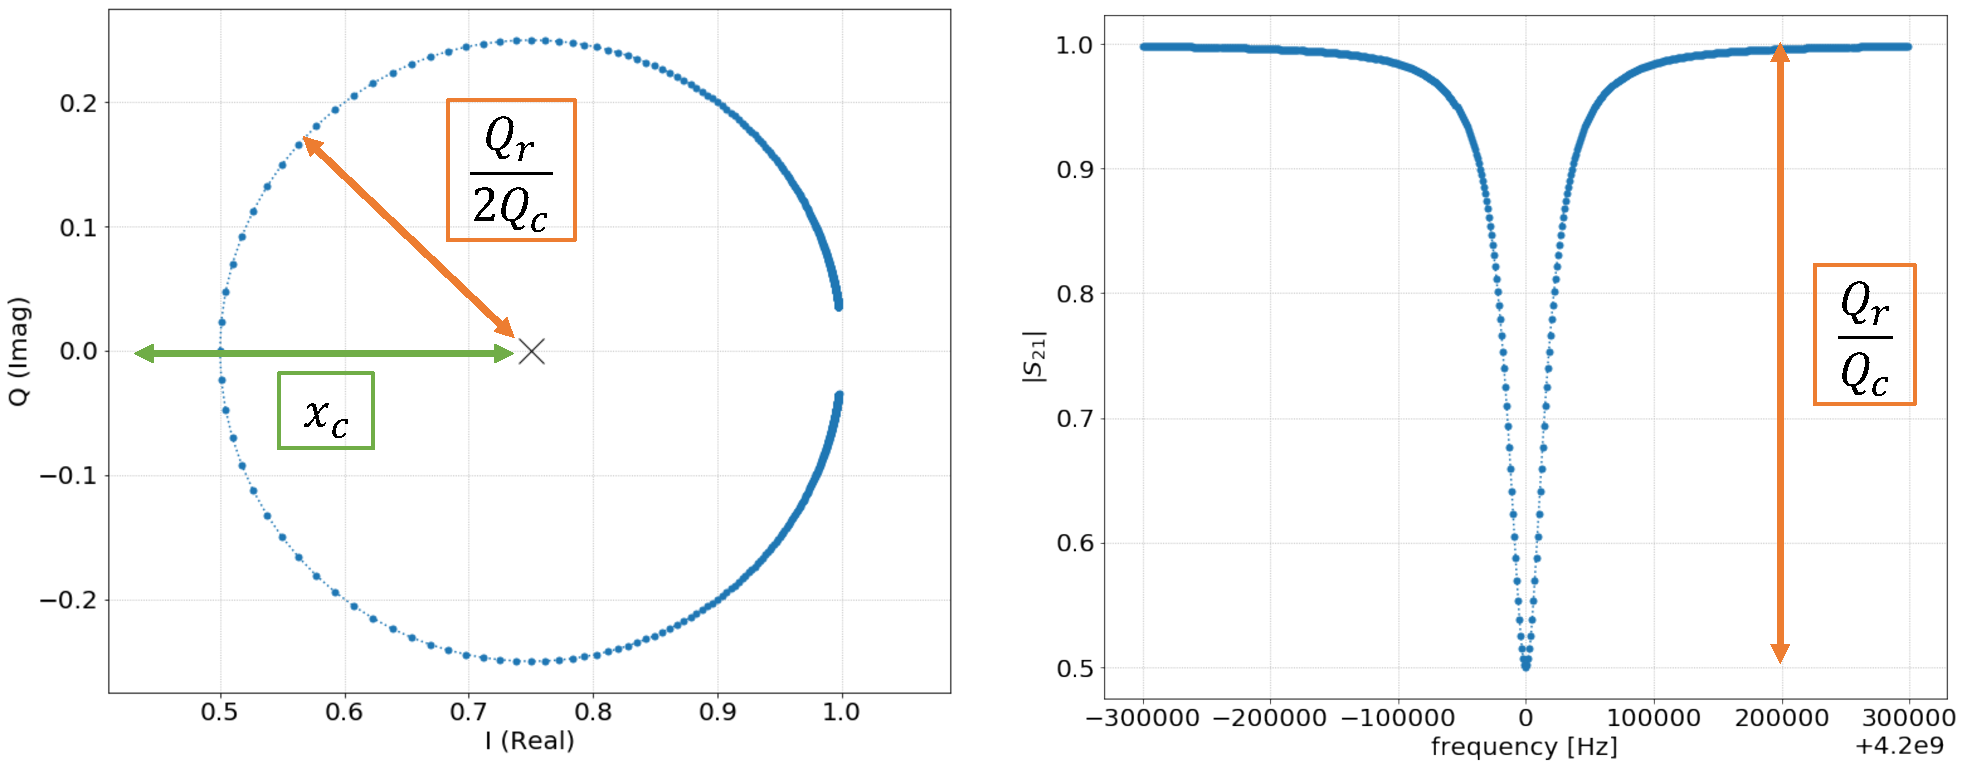
\includegraphics[width=0.9\columnwidth]{5_alignment/figs/iq_amp.pdf}
  %\caption{共振円と共振周波数付近での透過率。\cite{sueno_master}より引用。}
  %\label{res_circ}
%\end{figure}
%共振周波数の周りで透過率が鋭いピークを持つことが分かる。共振円を動く$S_{21}$の振幅$A$と位相$\theta$を
%\begin{equation}
  %A = \frac{|S_{21}|- x_{c}}{1-x_{c}}
%\end{equation}
%\begin{equation}
  %\tan\theta = \frac{\mathrm{Im}(S_{21})}{x_{c}- \mathrm{Re}(S_{21})}
%\end{equation}
%と定義する。これらの値は共振周波数の変化に対して敏感であるため、振幅の変化($\delta A$)と位相の変化($\delta\theta$)を測定することで入射信号の大きさを読み出せる。入射信号によって振幅と位相が変化する例を図\ref{amp_and_phase}に示す。
%\begin{figure}[htbp]
  %\centering
  %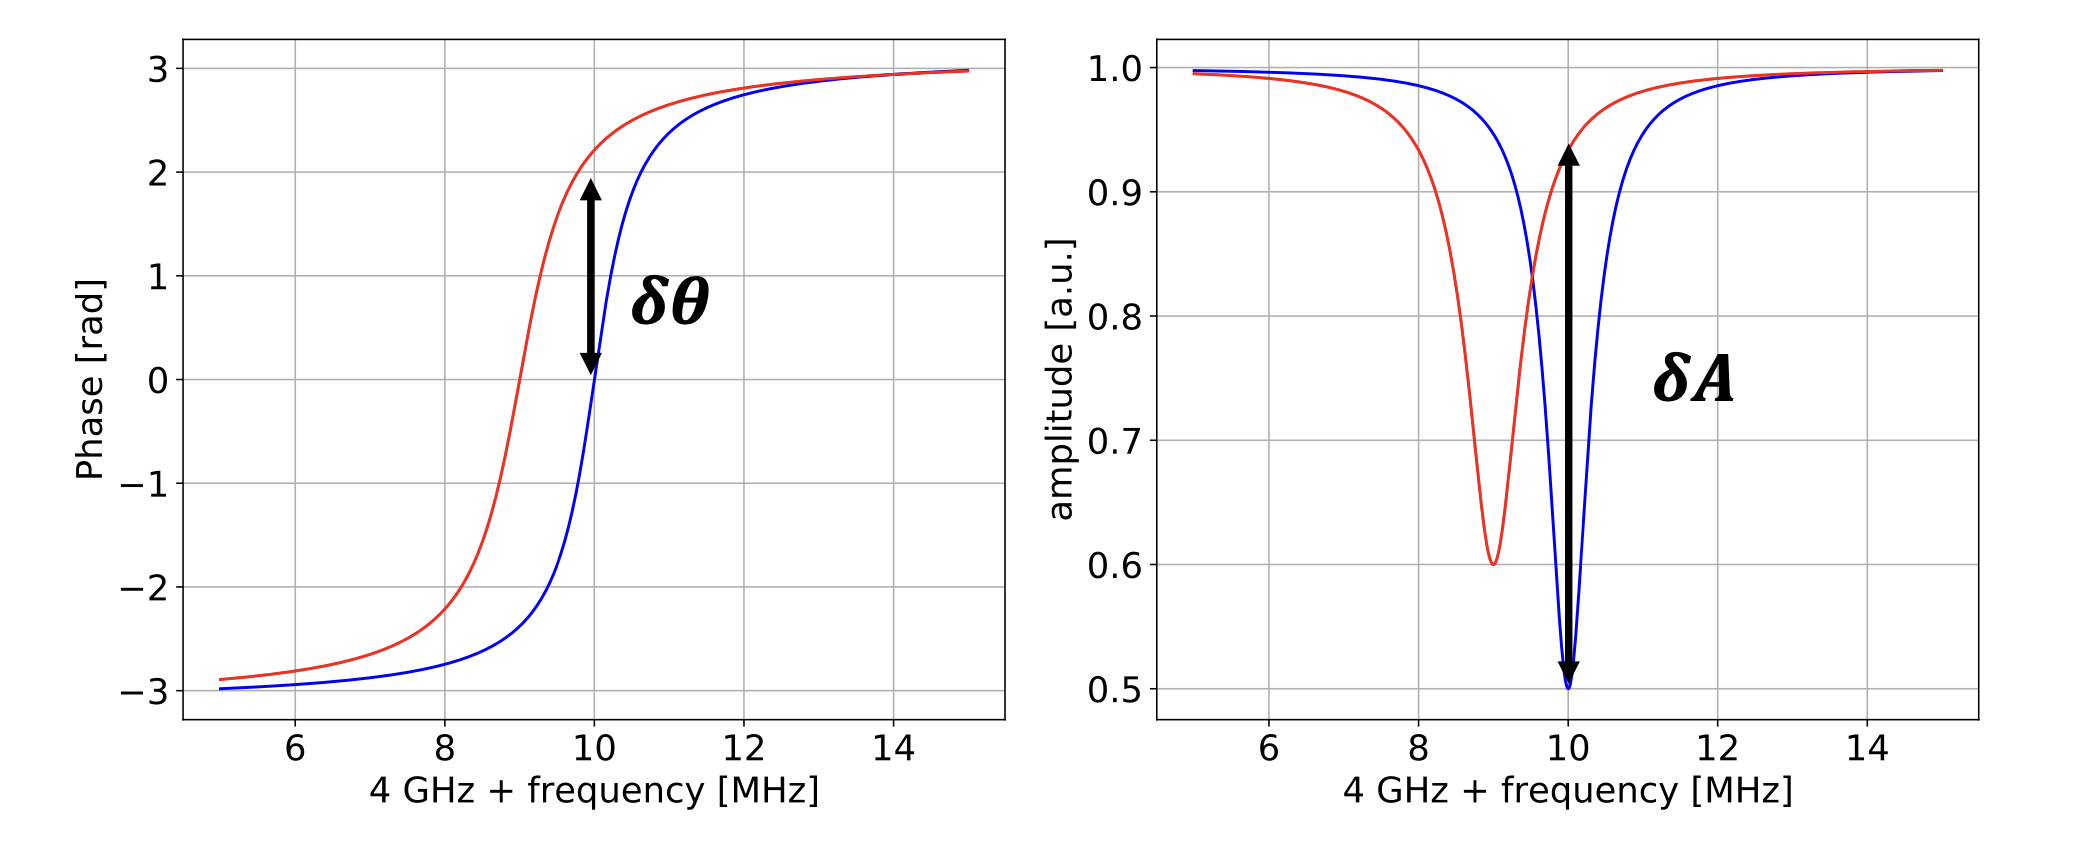
\includegraphics[width=1.0\columnwidth]{5_alignment/figs/amp_and_phase.png}
  %\caption{共振周波数付近での$S_{21}$の振幅と位相の変化。\cite{sueno_doctor}より引用。}
  %\label{amp_and_phase}
%\end{figure}
本論文ではより応答性の高い位相をTODとして使用する。また、非線形効果を補正したものを最終的に使用する位相TODとした。非線形効果の補正は位相の応答($\theta_{\mathrm{res}}$)に対して以下の式\cite{sueno_doctor}を用いた。
\begin{equation}
  \theta = 2\tan(\theta_{\mathrm{res}}/2)
\end{equation}
最終的に使用する位相TODの例(1観測)を図\ref{raw_phase}に示す。
\begin{figure}[htbp]
  \centering
  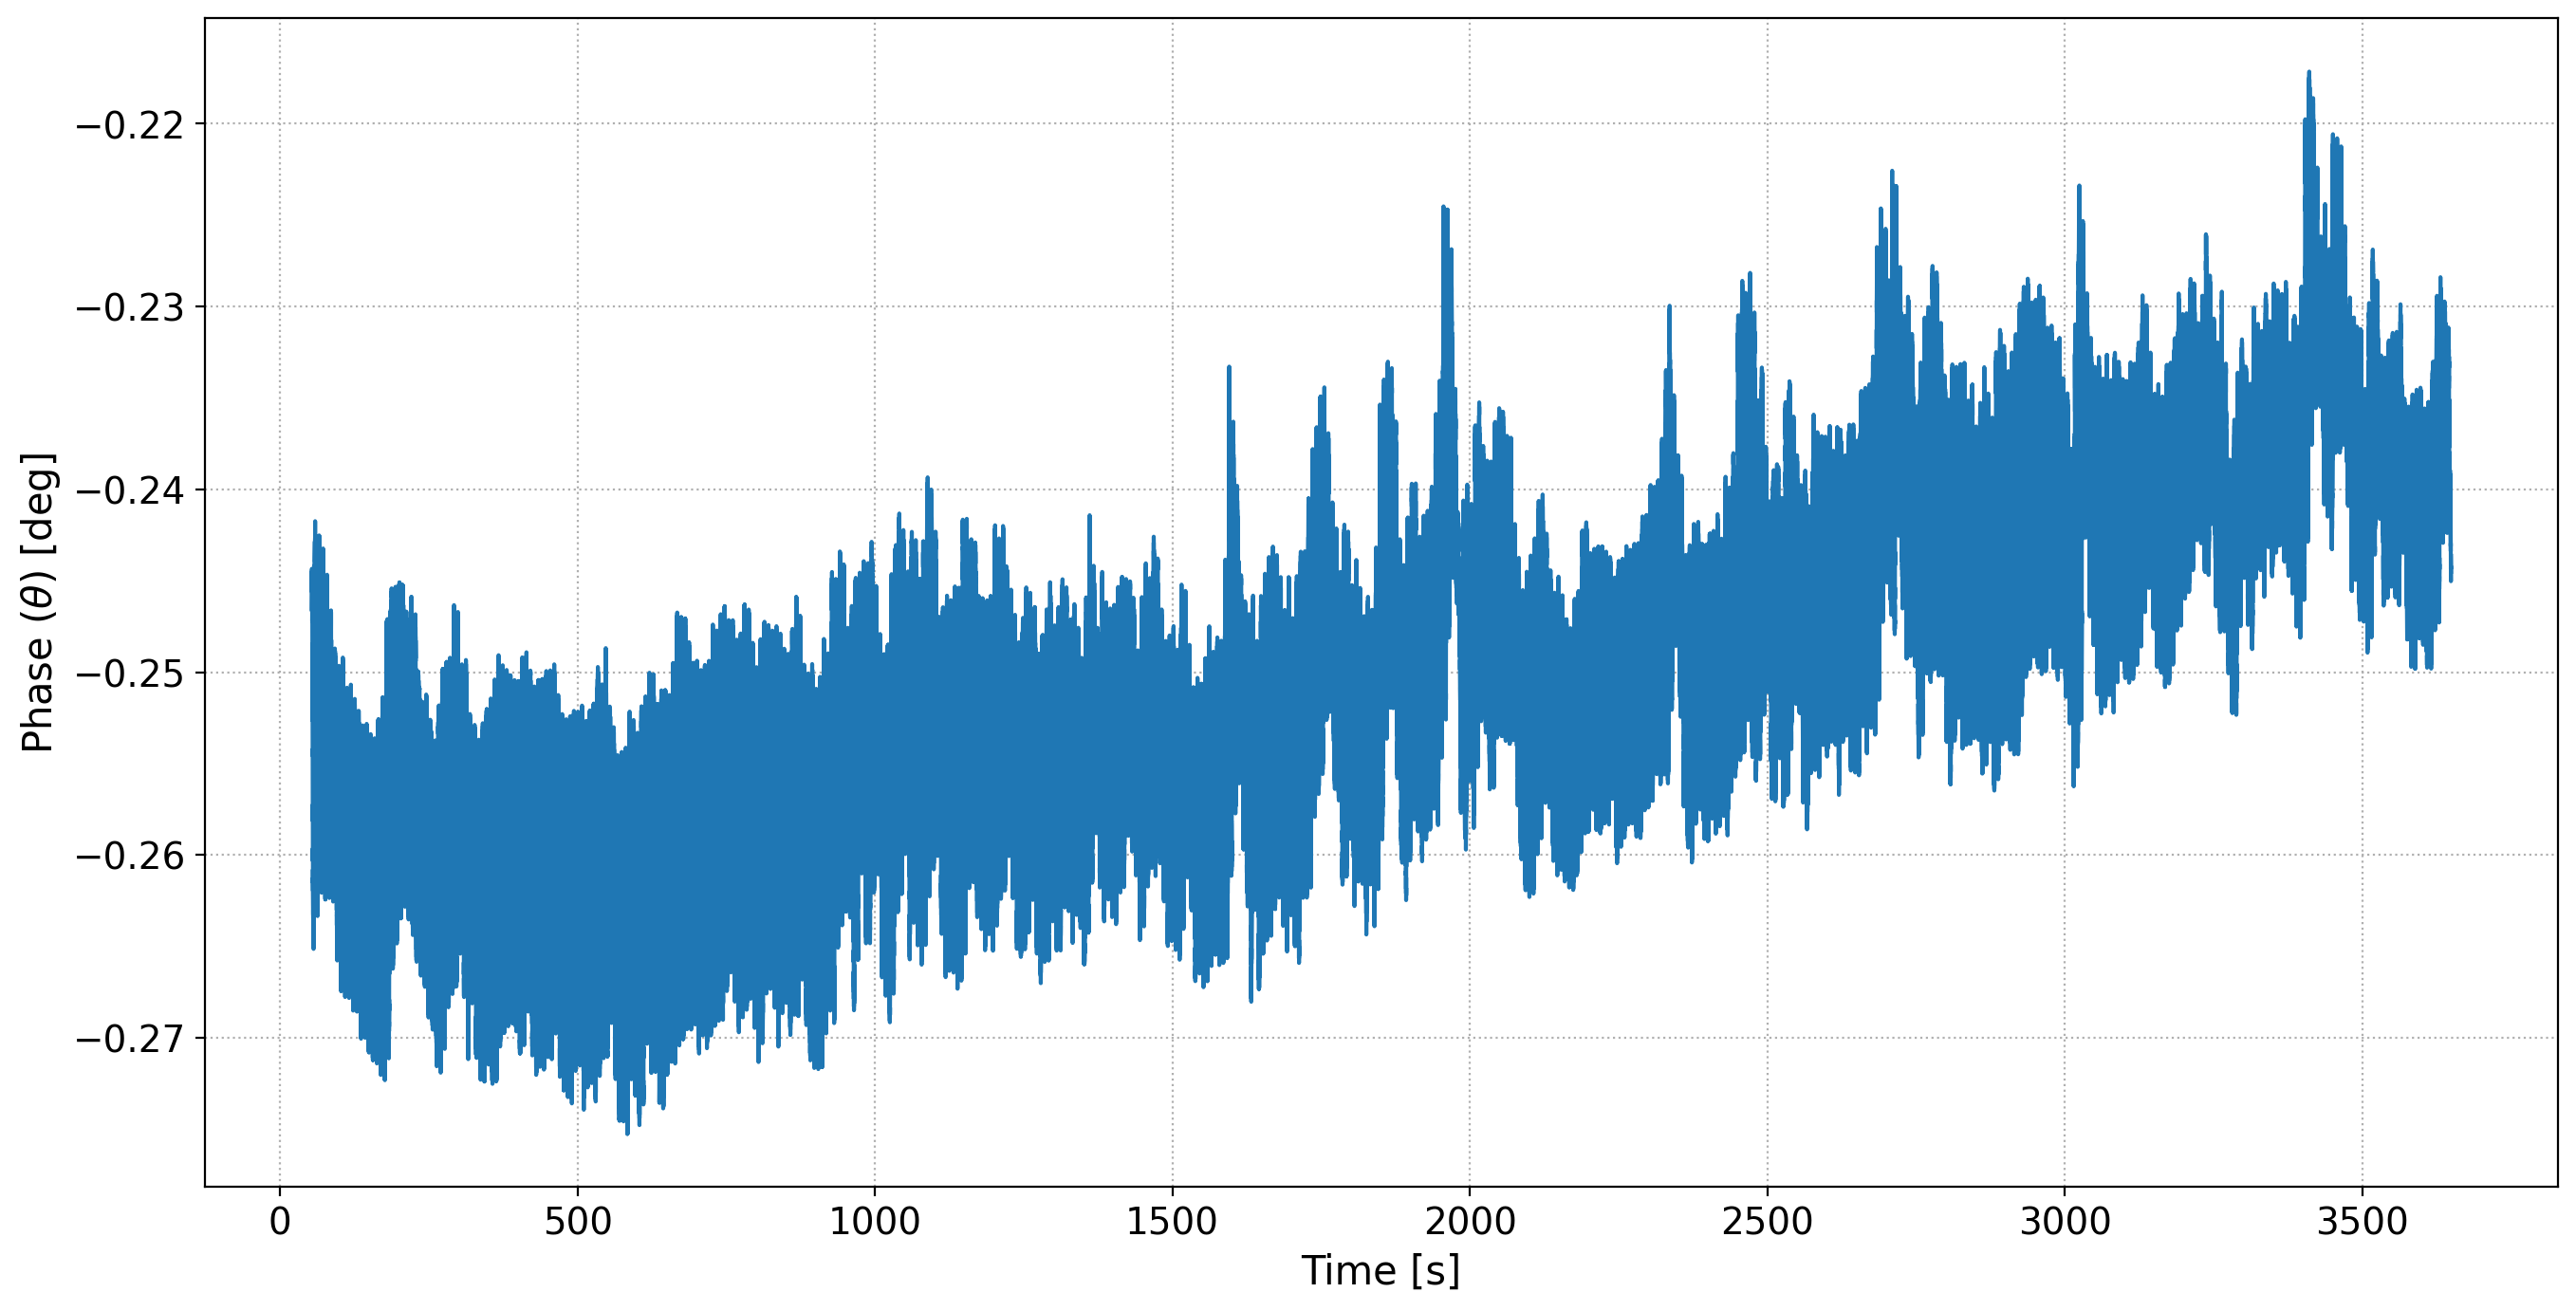
\includegraphics[width=0.9\columnwidth]{5_alignment/figs/raw_phase_deg.png}
  \caption{非線形効果を加えた位相TOD。本論文ではこのTODを用いる。}
  \label{raw_phase}
\end{figure}

\subsection{必要な回転角}
\label{angle_calculation}
月の信号は大きく1観測のTODで鮮明なマップを得ることができる。月を観測した時(2023/12/02、1時間)の位相TODを図\ref{6550_kid0_phase}に示す。
\begin{figure}[htbp]
  \centering
  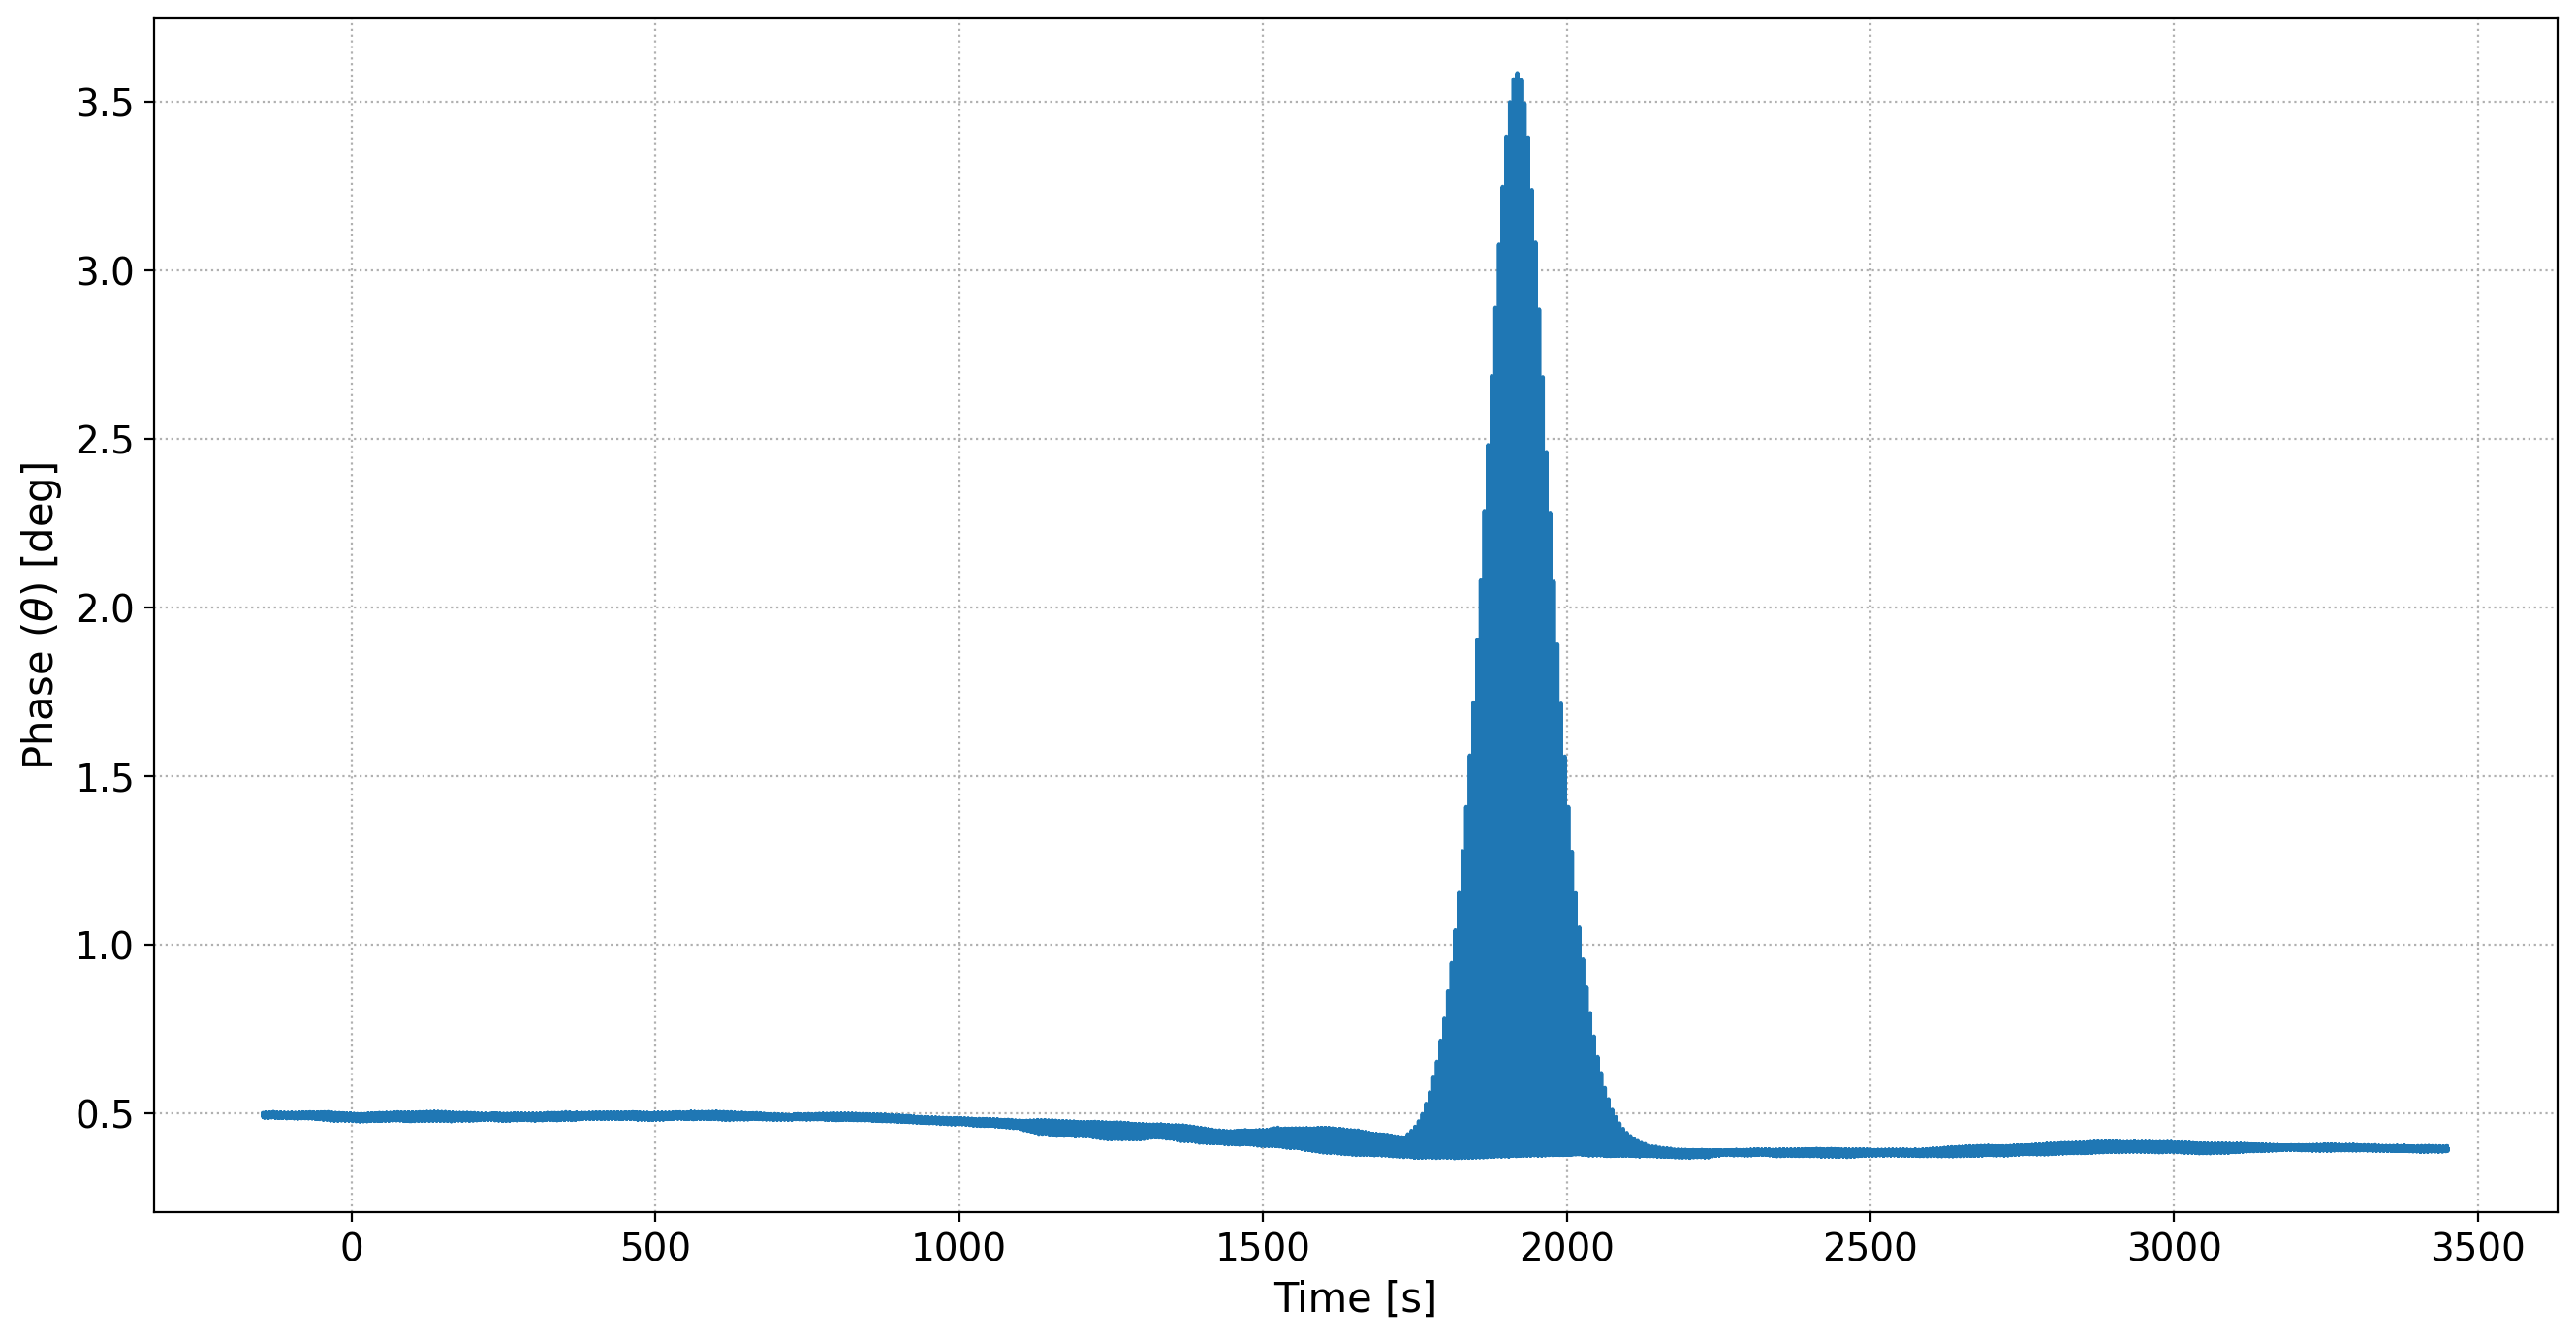
\includegraphics[width=0.85\columnwidth]{5_alignment/figs/6550_kid0_phase.png}
  \caption{月観測時のTOD。月の中心を観測した時にピークを取る。}
  \label{6550_kid0_phase}
\end{figure}
月は空を動いているが、望遠鏡が仰角を$\SI{70}{^{\circ}}$に固定してスキャンする間に月が望遠鏡の視野を通り過ぎる時に観測できる。つまり、1日の間に月が``昇る''時と``沈む''時とで2回の観測ができる。また、月の角直径は$\SI{30}{'}$であり点源とはみなせない。そのため図\ref{6550_kid0_phase}にあるように、月の端を観測する時と中心を観測する時では入射する信号の大きさが異なり、中心で最も強い信号を観測する。

月の運動はよく知られており、Pythonの``astropy\cite{astropy}''パッケージを使うことで各時間での月の位置(仰角、方位角)を求めることができる。その情報と望遠鏡角度情報とのずれ(オフセット)を考慮することでTODを月中心座標で表すことができ、月中心マップを構成することができる。\SI{220}{GHz}アレイの1観測から構成した各検出器の月中心マップを図\ref{moon_centered_6550}に示す。
\begin{figure}[htbp]
  \centering
  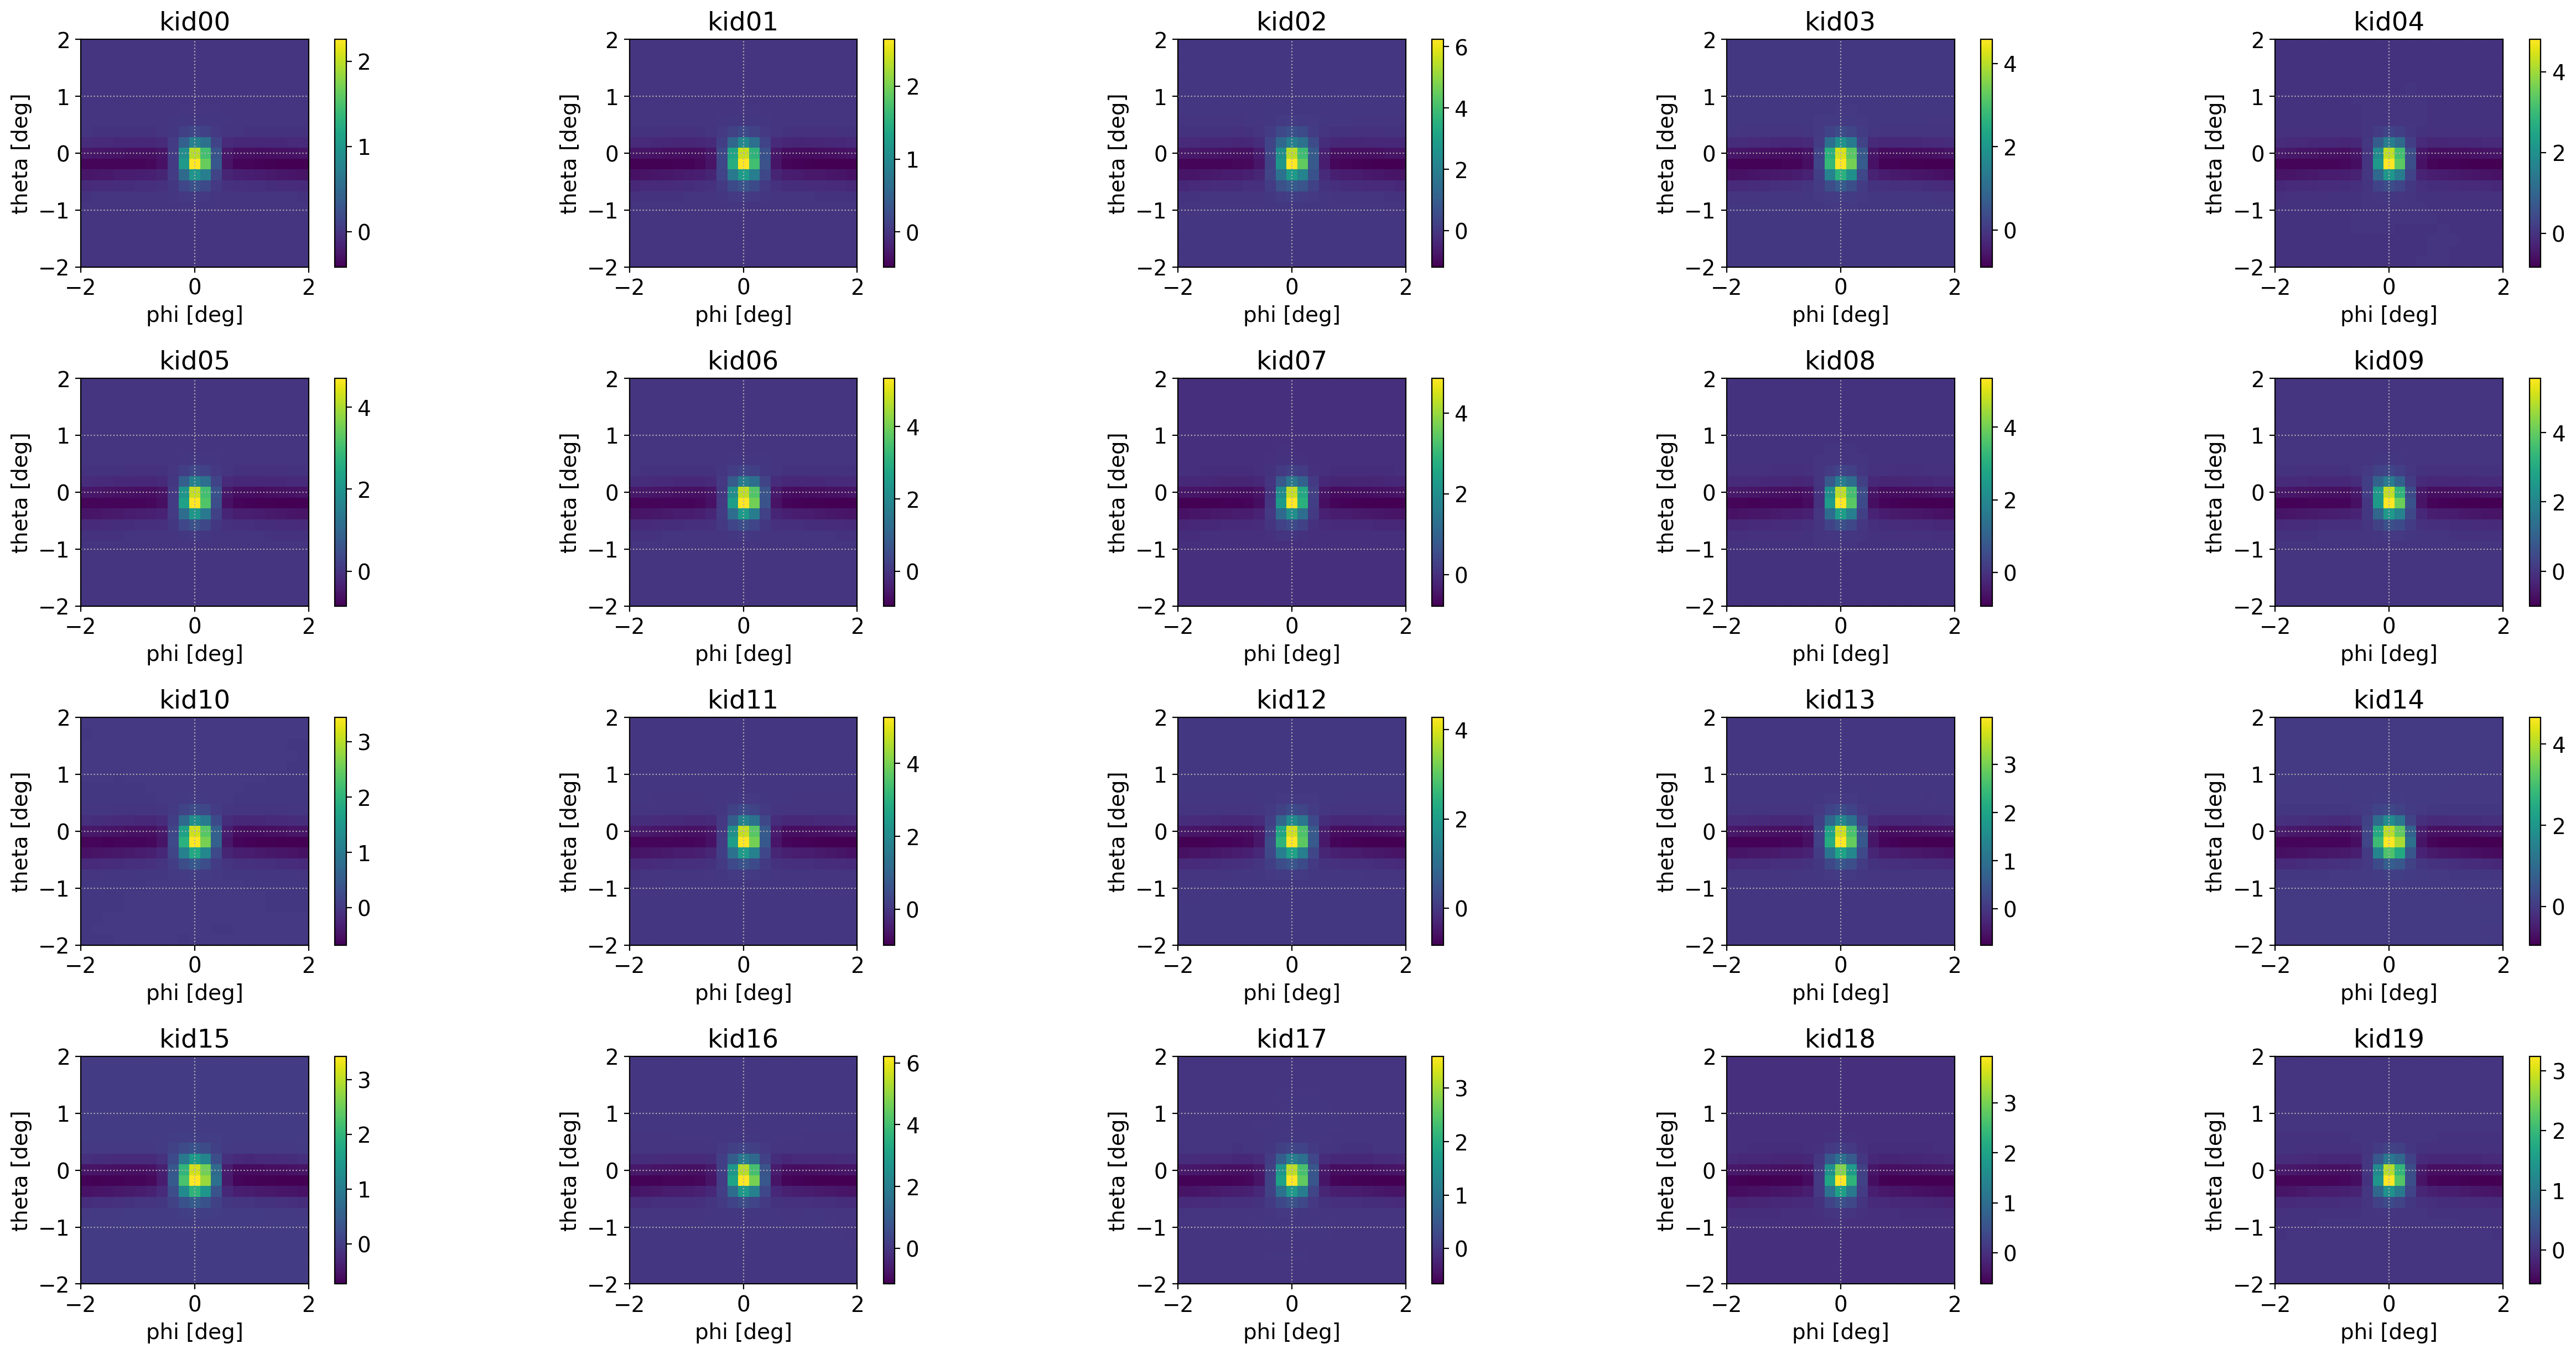
\includegraphics[width=0.85\columnwidth]{5_alignment/figs/moon_centered_6550.png}
  \caption{各MKIDの月中心マップ。座標中心(月中心)で位相が高くなる。}
  \label{moon_centered_6550}
\end{figure}

次にこの月中心のマップから各検出器が見ている空(視線)の情報を取得する。月中心マップでは検出器を個別に見ていたが、検出器全体としての視線情報を得るには望遠鏡の視線中心、つまりビームを中心とした時にどの位置で月を観測したかを知る必要がある。そのため、\SI{220}{GHz}アレイの中心にある検出器(kid17とラベルした)をビーム中心と考え、このビーム中心に対する月のマップを構成した。構成したマップの中で位相が最大となる位置を月の中心を見ていた位置として視線の代表点とする。\SI{220}{GHz}アレイのビーム中心マップと視線のプロットを図\ref{6550_beam_centered}に示す。
\begin{figure}[h]
  \begin{tabular}{cc}
    %---- 最初の図 ---------------------------
    \begin{minipage}[t]{0.48\hsize}
      \centering
      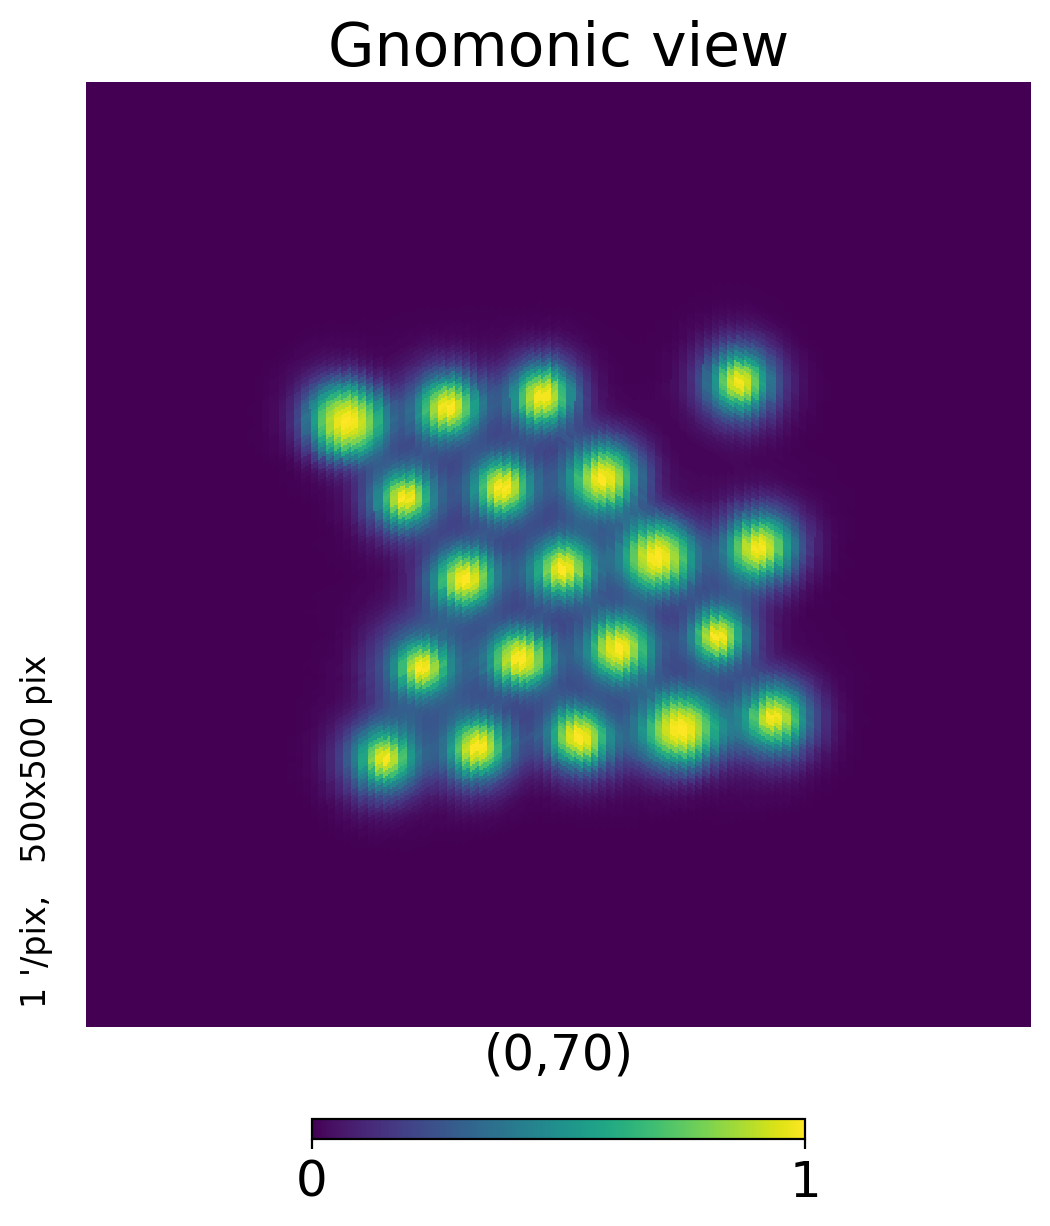
\includegraphics[keepaspectratio, scale=0.4]{5_alignment/figs/6550_gnomonic.png}
      \subcaption{\SI{220}{GHz}アレイのビーム中心マップ。}
      \label{6550_gnomview}
    \end{minipage}
    %---- 2番目の図 --------------------------
    \begin{minipage}[t]{0.48\hsize}
      \centering
      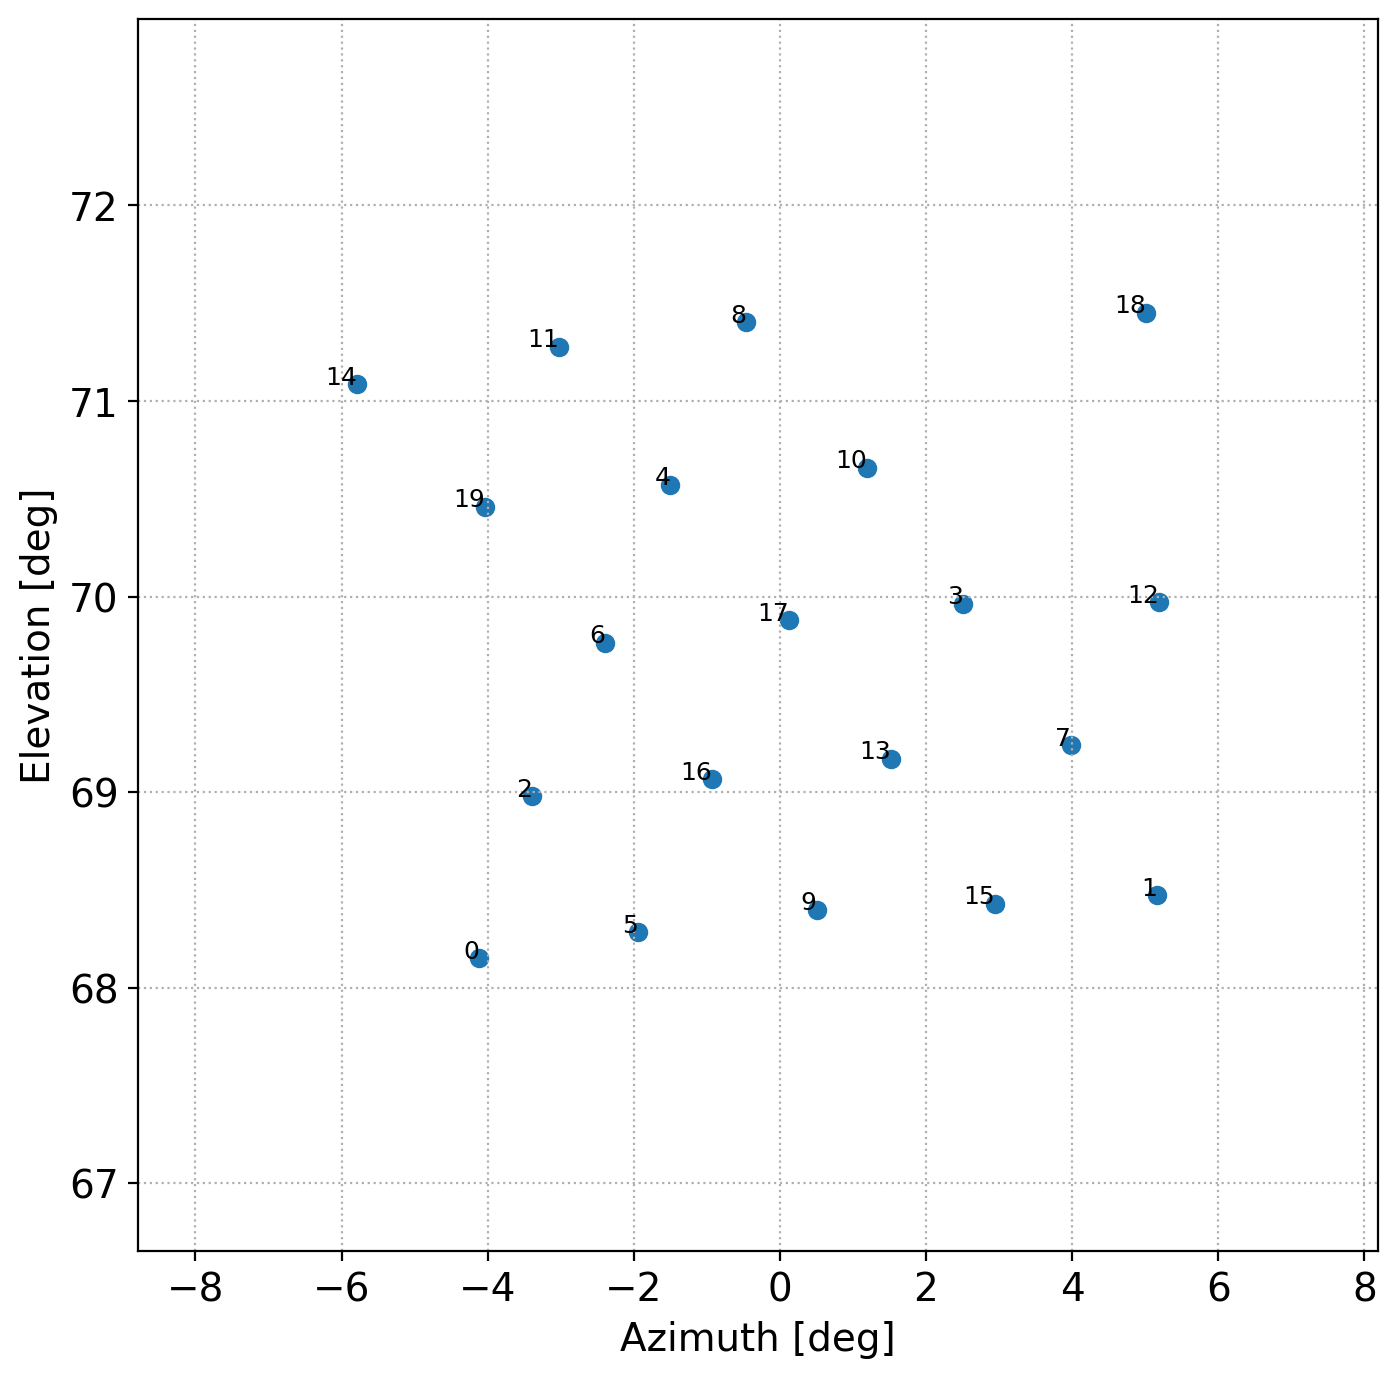
\includegraphics[keepaspectratio, scale=0.32]{5_alignment/figs/6550_pos_kid17_70.png}
      \subcaption{各検出器のビーム中心の視線。}
      \label{6550_pos}
    \end{minipage}
    %---- 図はここまで ----------------------
  \end{tabular}
  \caption{ビーム中心マップから取得した検出器の視線}
  \label{6550_beam_centered}
\end{figure}
ここで\ref{6550_gnomview}では``healpy\cite{healpy}''のgnomviewを使って球面のマップを平面射影している。また、\ref{6550_pos}には検出器のラベルとして各点に番号を記した。この図から検出器の配置がスキャン軸に対して傾いていることが見て取れる。また、中心アレイでは仰角$\SI{70}{^{\circ}}$でも球面による歪みが少なく平面的に見えている。

加えて中心以外の\SI{145}{GHz}アレイも含めた検出器全体でのビーム中心マップを見て傾きを確認した。TODは同時刻帯の月を観測した時のものを使用した。使用データを表\ref{before_full_array_table}に示す。
\begin{table}[htbp]
  \centering
  \caption{ビーム中心マップの構成に使用した月観測データ}
  \vspace{3mm}
  \begin{tabular}{cccc} \hline
    観測日(UTC) & 観測時間 [min] & 周波数 [GHz] & 月の昇降(rise or set) \\ \hline
    2024/02/22 0:04 - 1:04 & 60 & 145 & set \\
    2024/02/22 0:17 - 1:17 & 60 & 145 & set \\
    2024/02/22 0:18 - 1:18 & 60 & 145 & set \\
    2024/02/22 0:37 - 1:37 & 60 & 220 & set \\
    2024/02/22 0:48 - 1:48 & 60 & 145 & set \\
    2024/02/22 0:48 - 1:48 & 60 & 145 & set \\
    2024/02/22 1:10 - 2:10 & 60 & 145 & set \\ \hline

  \end{tabular}
  \label{before_full_array_table}
\end{table}
ビーム中心マップと全検出器の視線は図\ref{6550_beam_centered}と同じ計算で求めた(図\ref{before_full_beam_map}と図\ref{before_full_beam_pos})。
%\begin{figure}[h]
  %\begin{tabular}{cc}
    %---- 最初の図 ---------------------------
    %\begin{minipage}[t]{0.48\hsize}
      %\centering
      %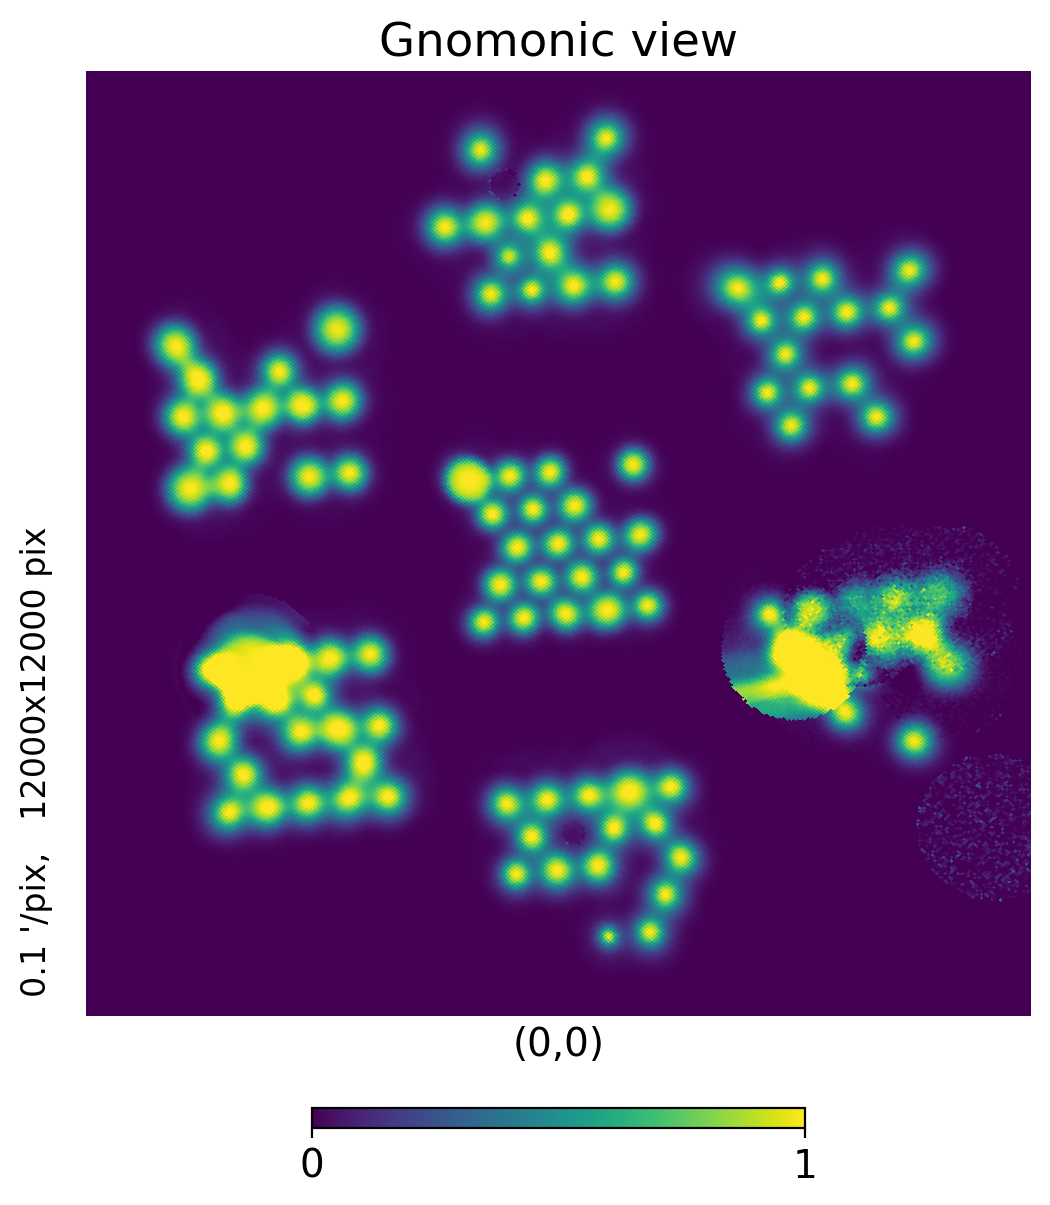
\includegraphics[keepaspectratio, scale=0.4]{5_alignment/figs/before_full_gnomonic.png}
      %\subcaption{フルアレイのビーム中心マップ。}
      %\label{before_full_beam_map}
    %\end{minipage}
    %---- 2番目の図 --------------------------
    %\begin{minipage}[t]{0.48\hsize}
      %\centering
      %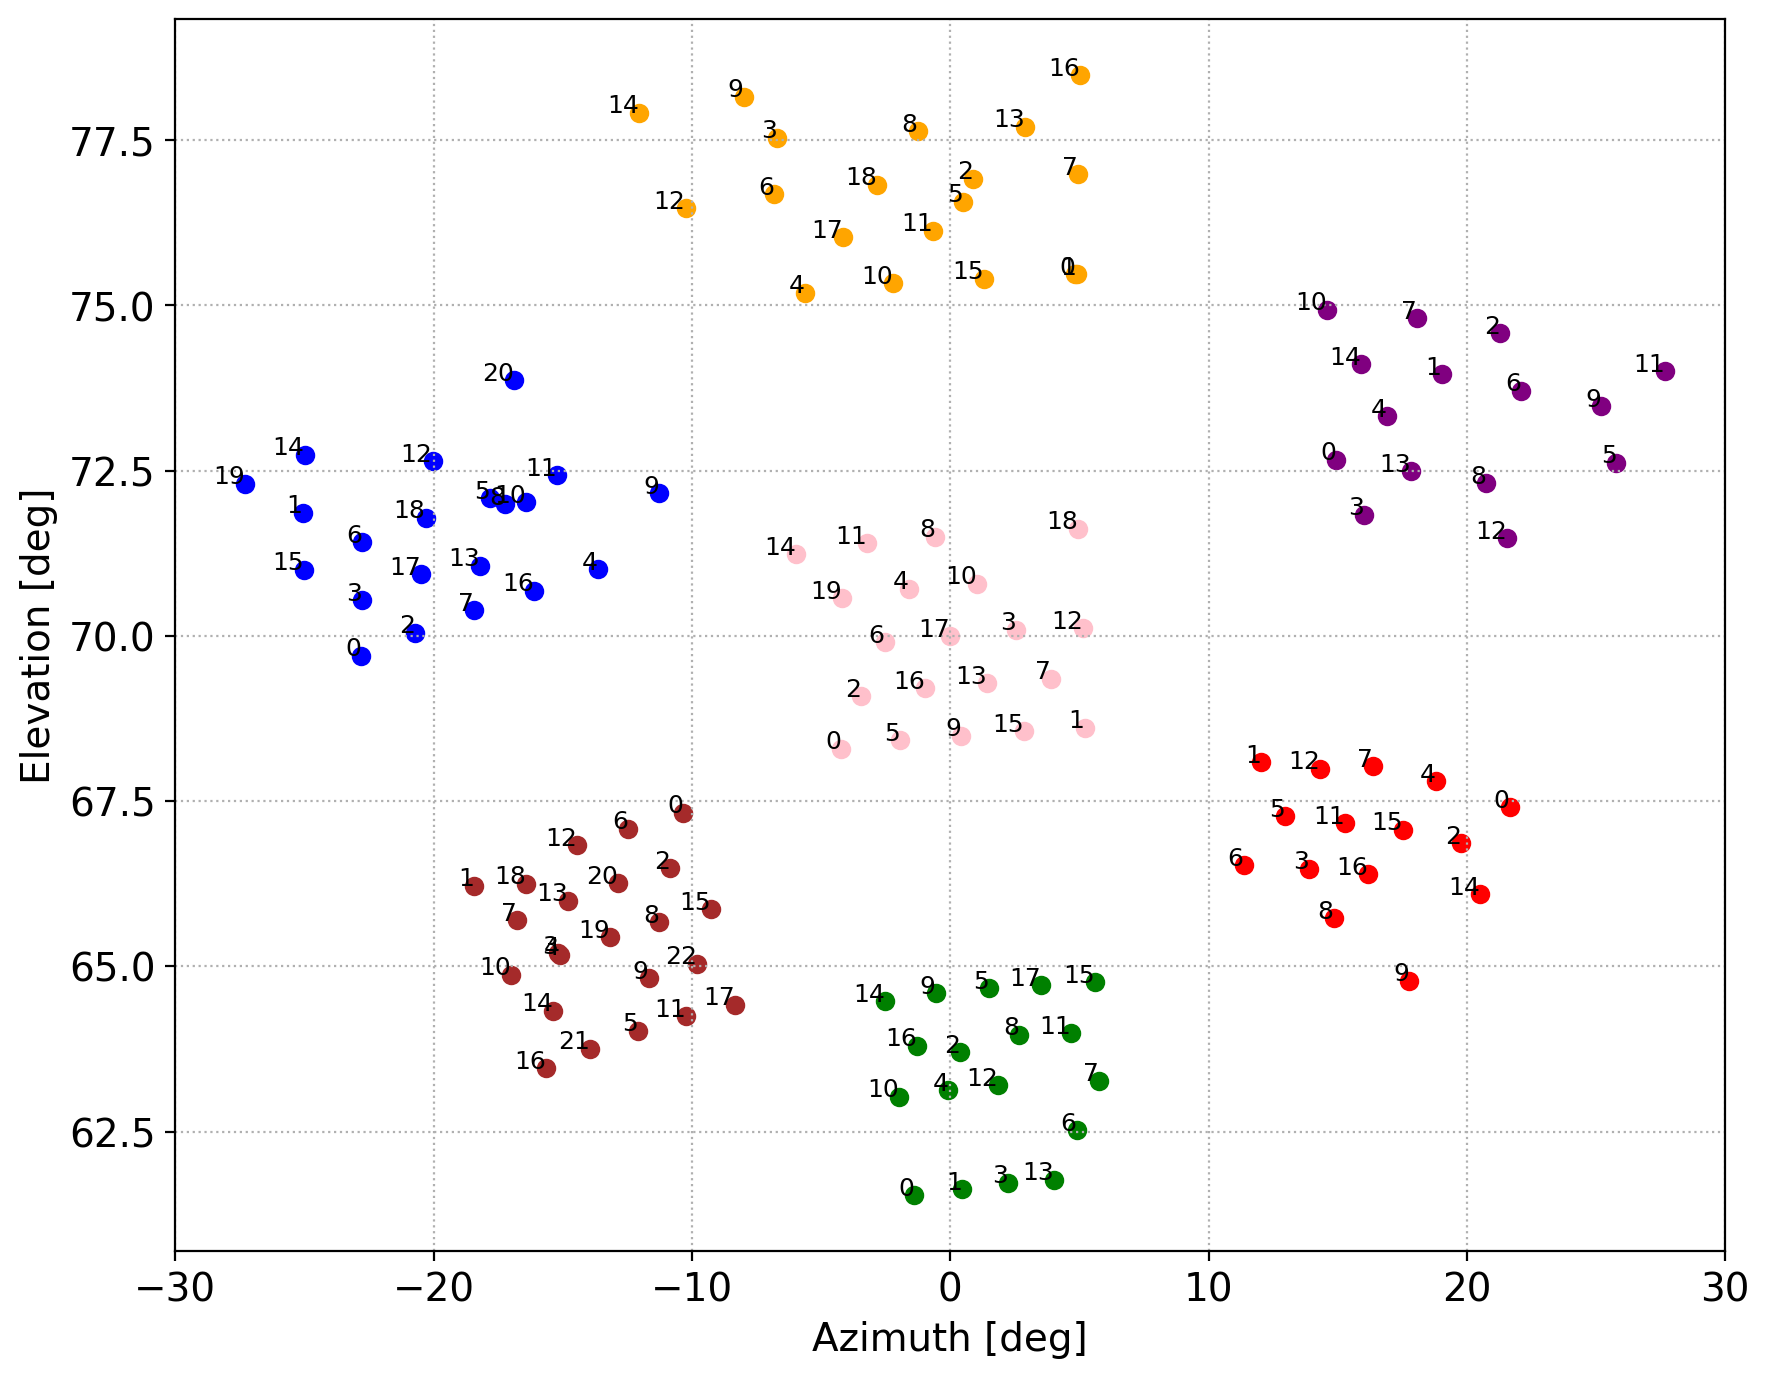
\includegraphics[keepaspectratio, scale=0.32]{5_alignment/figs/before_full_pos_70.png}
      %\subcaption{全検出器のビーム中心の視線。}
      %\label{before_full_pos_70}
    %\end{minipage}
    %---- 図はここまで ----------------------
  %\end{tabular}
  %\caption{ビーム中心マップから取得した全検出器の視線}
  %\label{before_full_beam_centered}
%\end{figure}
\begin{figure}[htbp]
  \centering
  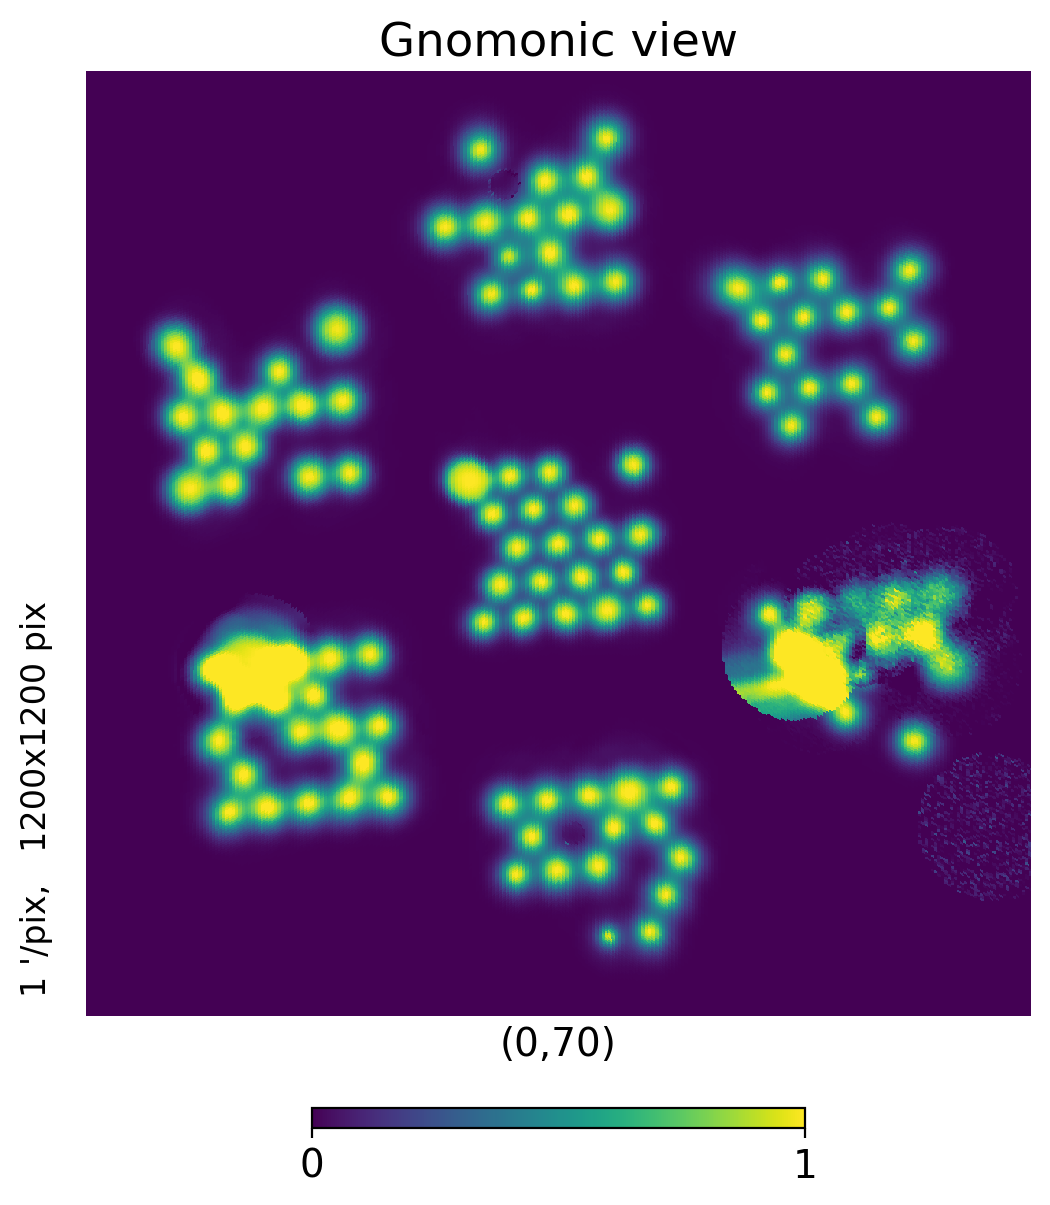
\includegraphics[width=0.7\columnwidth]{5_alignment/figs/before_full_gnomonic_70.png}
  \caption{フルアレイのビーム中心マップ。左右の\SI{145}{GHz}アレイで見られるように一部の検出器では月のマップが重なることがあり、視線情報の再構成が上手くできない。}
  \label{before_full_beam_map}
\end{figure}
\begin{figure}[htbp]
  \centering
  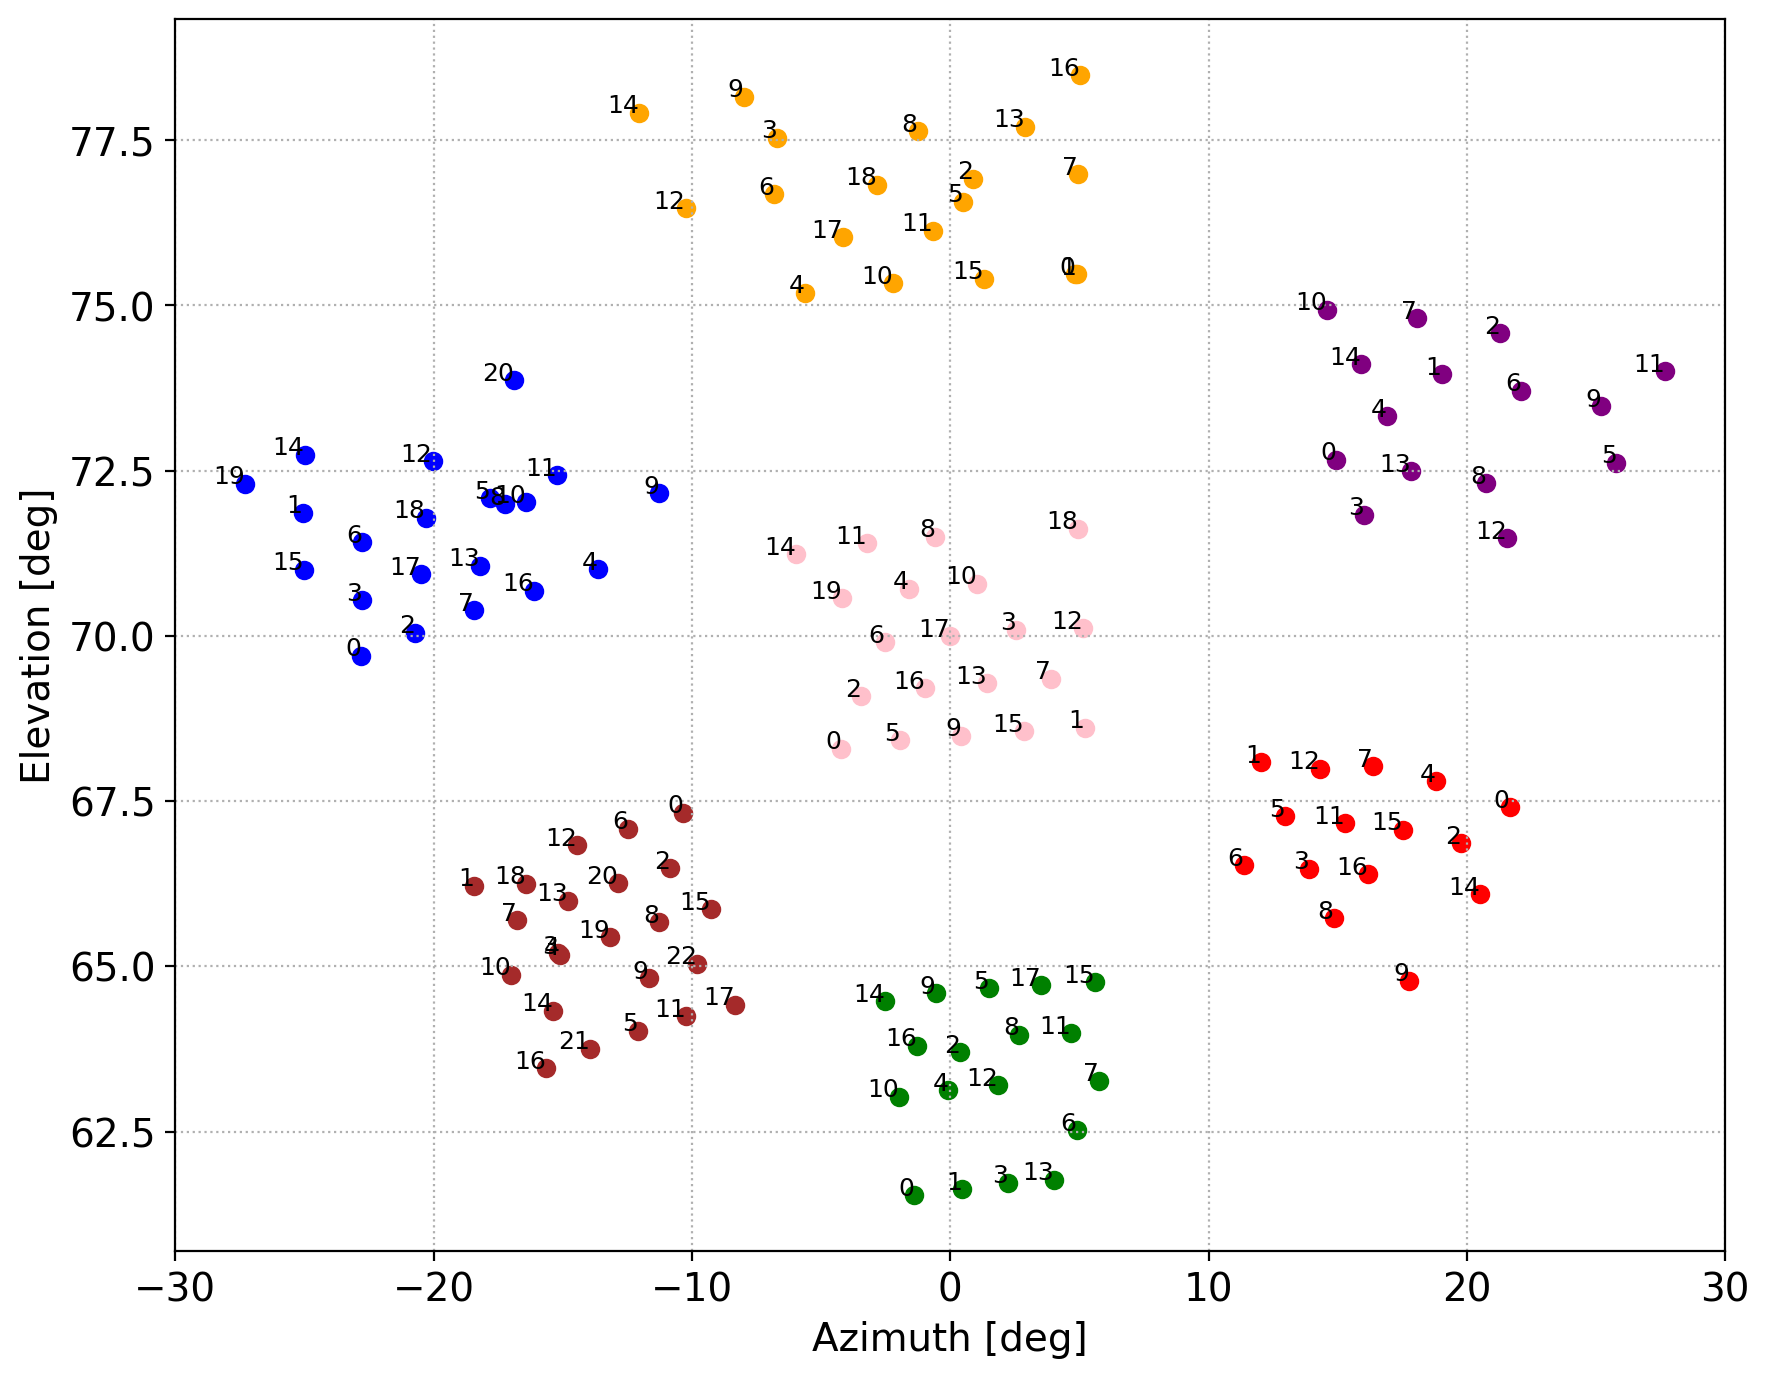
\includegraphics[width=1.0\columnwidth]{5_alignment/figs/before_full_pos_70.png}
  \caption{全検出器のビーム中心の視線。各点の番号は検出器のラベルとして記しており、中心の\SI{220}{GHz}アレイのkid17をビーム中心としている。中心以外の\SI{145}{GHz}アレイでは球面に起因する位置の歪みが現れる。}
  \label{before_full_beam_pos}
\end{figure}
全検出器で視線を見ると、図\ref{distortion_pos}で示したような天球面での歪みの効果が周りのアレイに表れる。仰角が$\SI{90}{^{\circ}}$に近づくにつれて検出器が見ている角度の間隔が広くなる。全体としてビーム中心に対して傾いていることが見て取れる。歪みの効果を補正するために仰角を$\SI{70}{^{\circ}}$から$\SI{0}{^{\circ}}$に天球面上で回転させた全検出器の視線を図\ref{before_full_pos_0}に示す。
\begin{figure}[htbp]
  \centering
  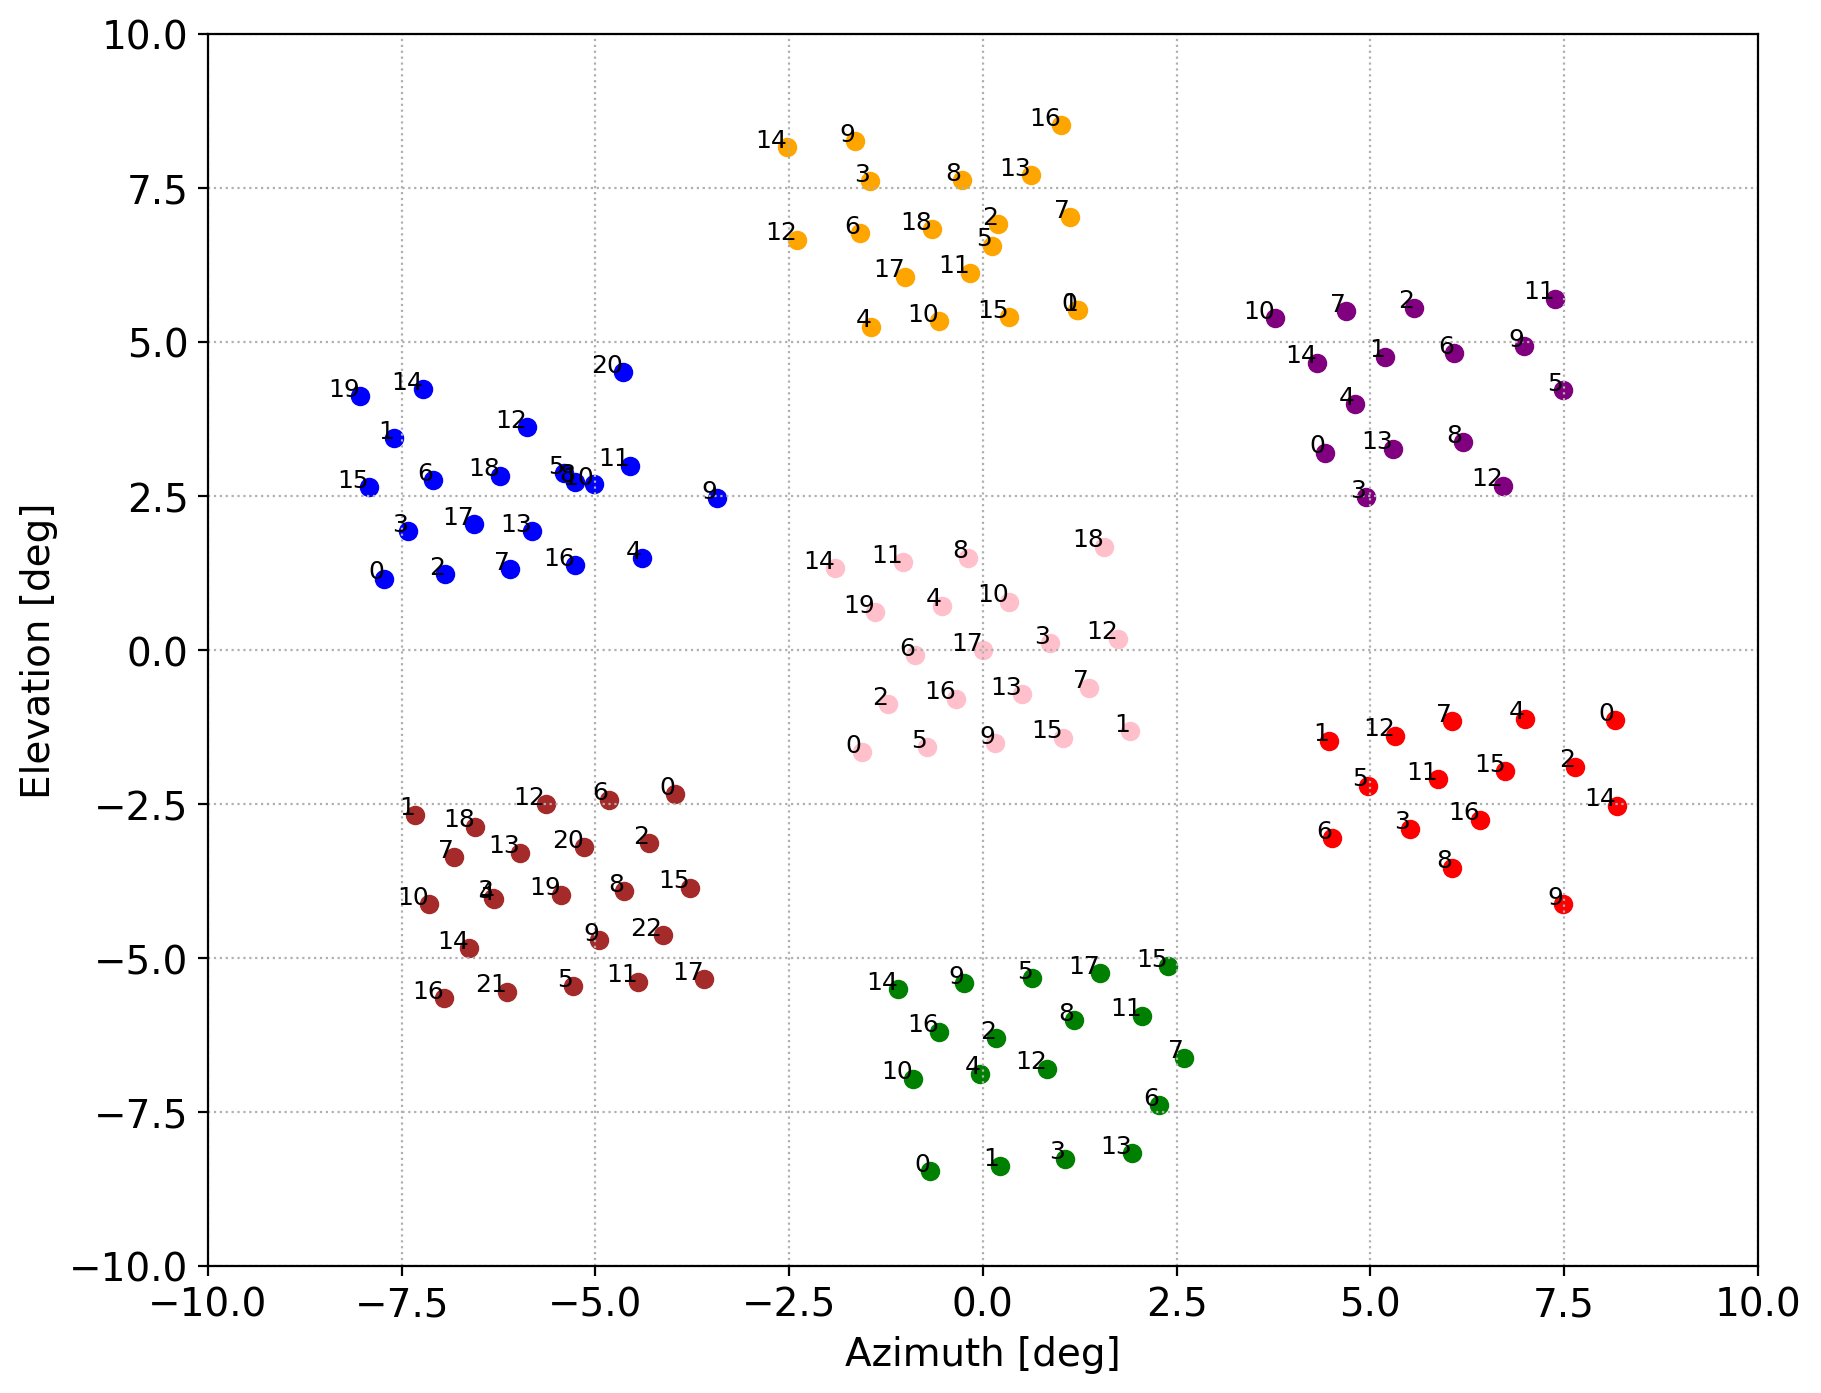
\includegraphics[width=1.0\columnwidth]{5_alignment/figs/before_full_pos.png}
  \caption{座標回転により平面的に見たビーム中心の視線。}
  \label{before_full_pos_0}
\end{figure}
回転角を見積もるにあたってはスキャン軸に対する検出器の傾きを直線的に扱える方が考えやすい。そのため、平面的に見た時の傾き角を計算し、較正のための回転角とする。

回転角の算出には歪みの効果が少ない中心の\SI{220}{GHz}アレイのみを使用する。また、中心アレイはスキャン軸に対して5列で検出器が並んでいて理想的には全ての列が同じ角度で傾いていることになる。それを踏まえて以下の手順で回転角を求めた。
\begin{enumerate}
  \item 複数日での月観測データ(\SI{220}{GHz}アレイ)から検出器の視線を求める
  \item アレイ内で5列に並ぶ検出器のそれぞれの列で位置を直線フィット(データの性質が良くなかった1列目は省略した)
  \item フィットの傾きをその列での回転角としてヒストグラムに詰めて、ヒストグラムをガウシアンでフィット
  \item ガウシアン中心を最終的な回転角とする
\end{enumerate}
角度決定における信頼性を高めるために複数の観測データを使用した。表\ref{angle_cal_tods}に使用した\SI{220}{GHz}アレイの月観測データをまとめる。
\begin{table}[htbp]
  \centering
  \caption{回転角の決定に使用した月観測データ}
  \vspace{3mm}
  \begin{tabular}{ccc} \hline
    観測日(UTC) & 観測時間 [min]  & 月の昇降(rise or set) \\ \hline
    2023/06/15 9:04 - 10:04 & 60 & rise \\
    2023/12/02 3:06 - 4:06 & 60 & rise \\
    2023/12/02 6:09 - 7:09 & 60 & set \\
    2023/12/04 4:59 - 5:59 & 60 & rise \\
    2023/12/04 7:06 - 8:06 & 60 & set \\
    2023/12/27 2:12 - 3:12 & 60 & set \\
    2024/02/21 21:34 - 22:34 & 60 & rise \\
    2024/02/22 0:37 - 1:37 & 60 & set \\
    2024/07/01 6:48 - 7:48 & 60 & rise \\
    2024/07/02 7:59 - 8:59 & 60 & rise \\ \hline

  \end{tabular}
  \label{angle_cal_tods}
\end{table}
各観測データで検出器の列ごとに行った回転角の直線フィットを図\ref{linear_fit}に示す。
\begin{figure}[htbp]
  \centering
  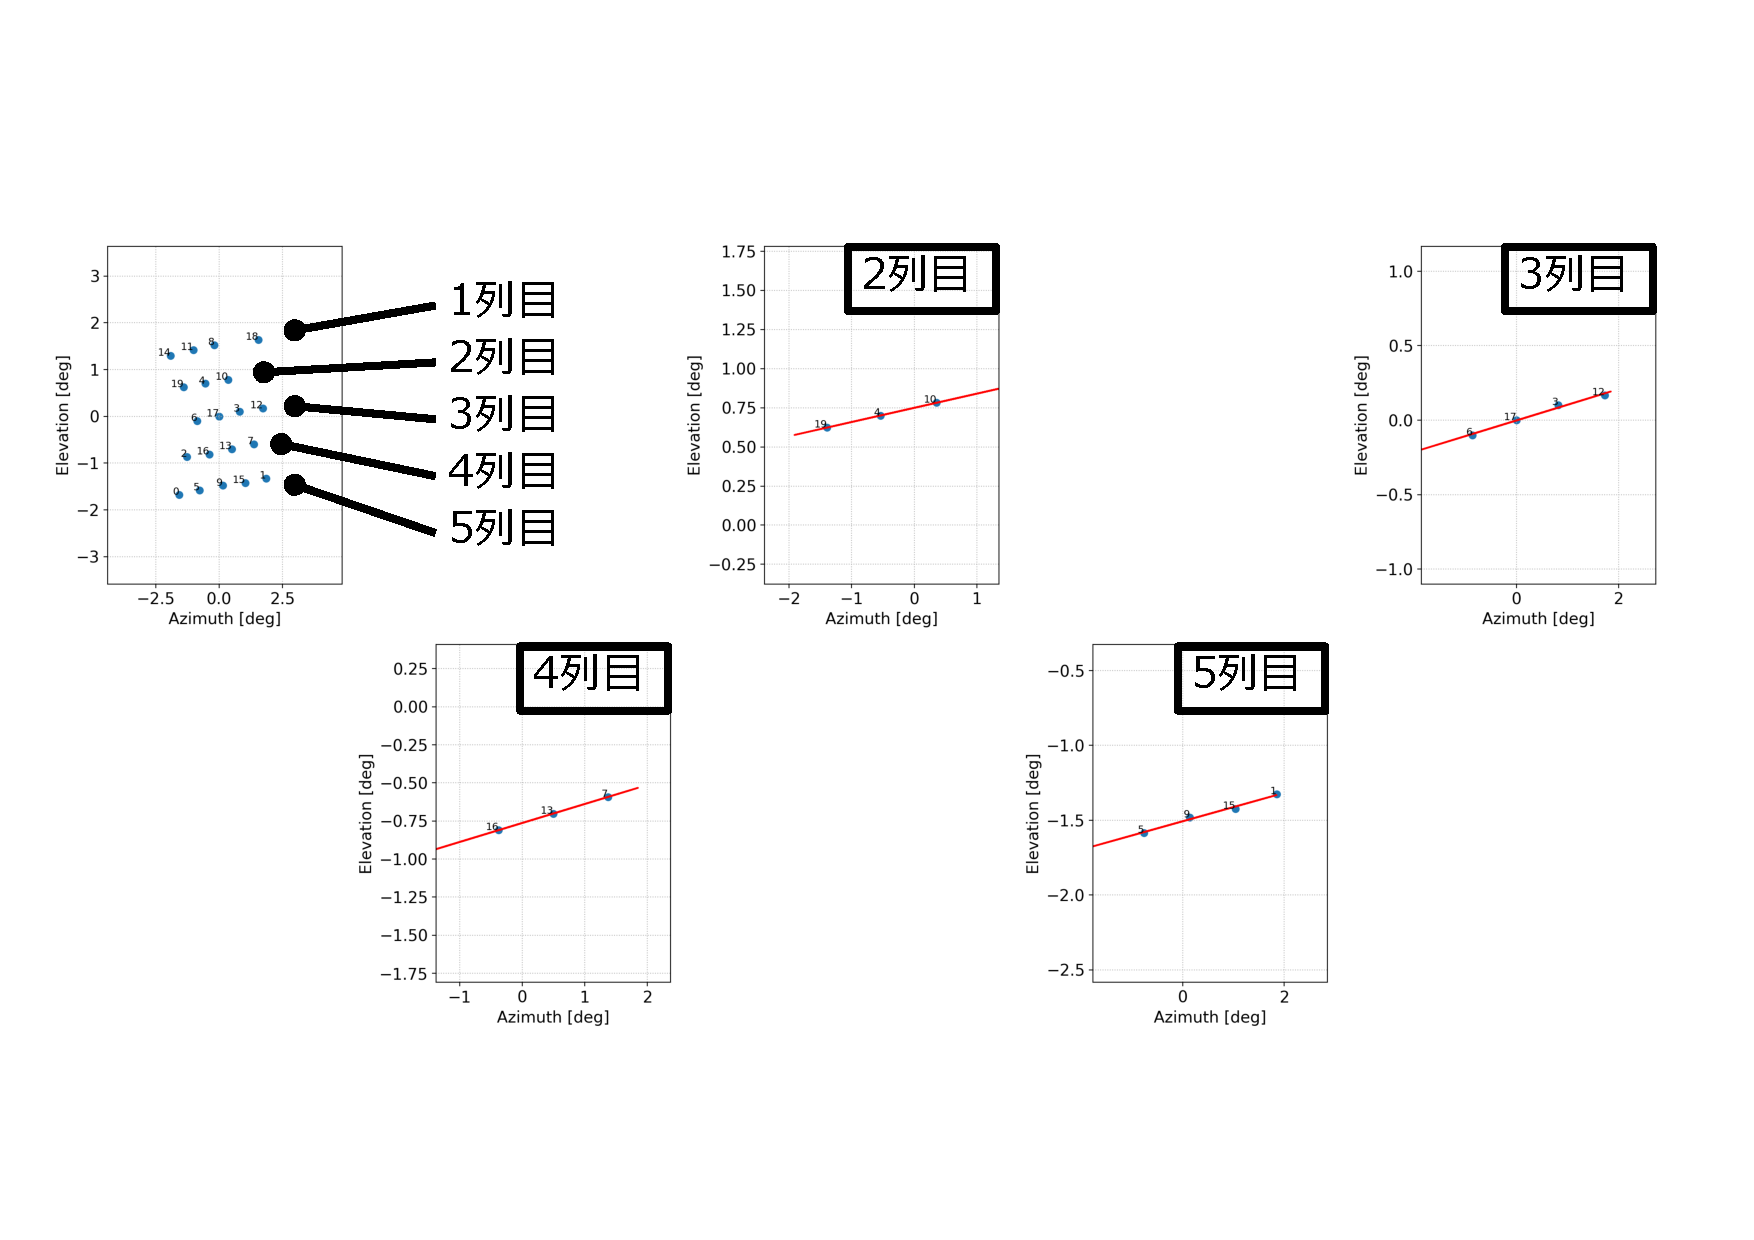
\includegraphics[width=1.05\columnwidth]{5_alignment/figs/angle_cal_lines.pdf}
  \caption{検出器の各列での直線フィット。全5列の内、1列目は除外した。}
  \label{linear_fit}
\end{figure}
アレイの1列目について、データの性質が良くなく視線の再構成に失敗した検出器が複数の観測で見られたため、使用しなかった。そのため1観測で2~5列目までの4列でそれぞれ直線の傾きから回転角を算出した。また、10観測分の月データについて同様の手順を踏んだため、合計で40の回転角データを求めた。この回転角の中で明らかな外れ値があったため除外し、最終的に38の回転角データを得た。回転角ヒストグラムのガウシアンフィットの結果を図\ref{gaussian_fit}に示す。
\begin{figure}[htbp]
  \centering
  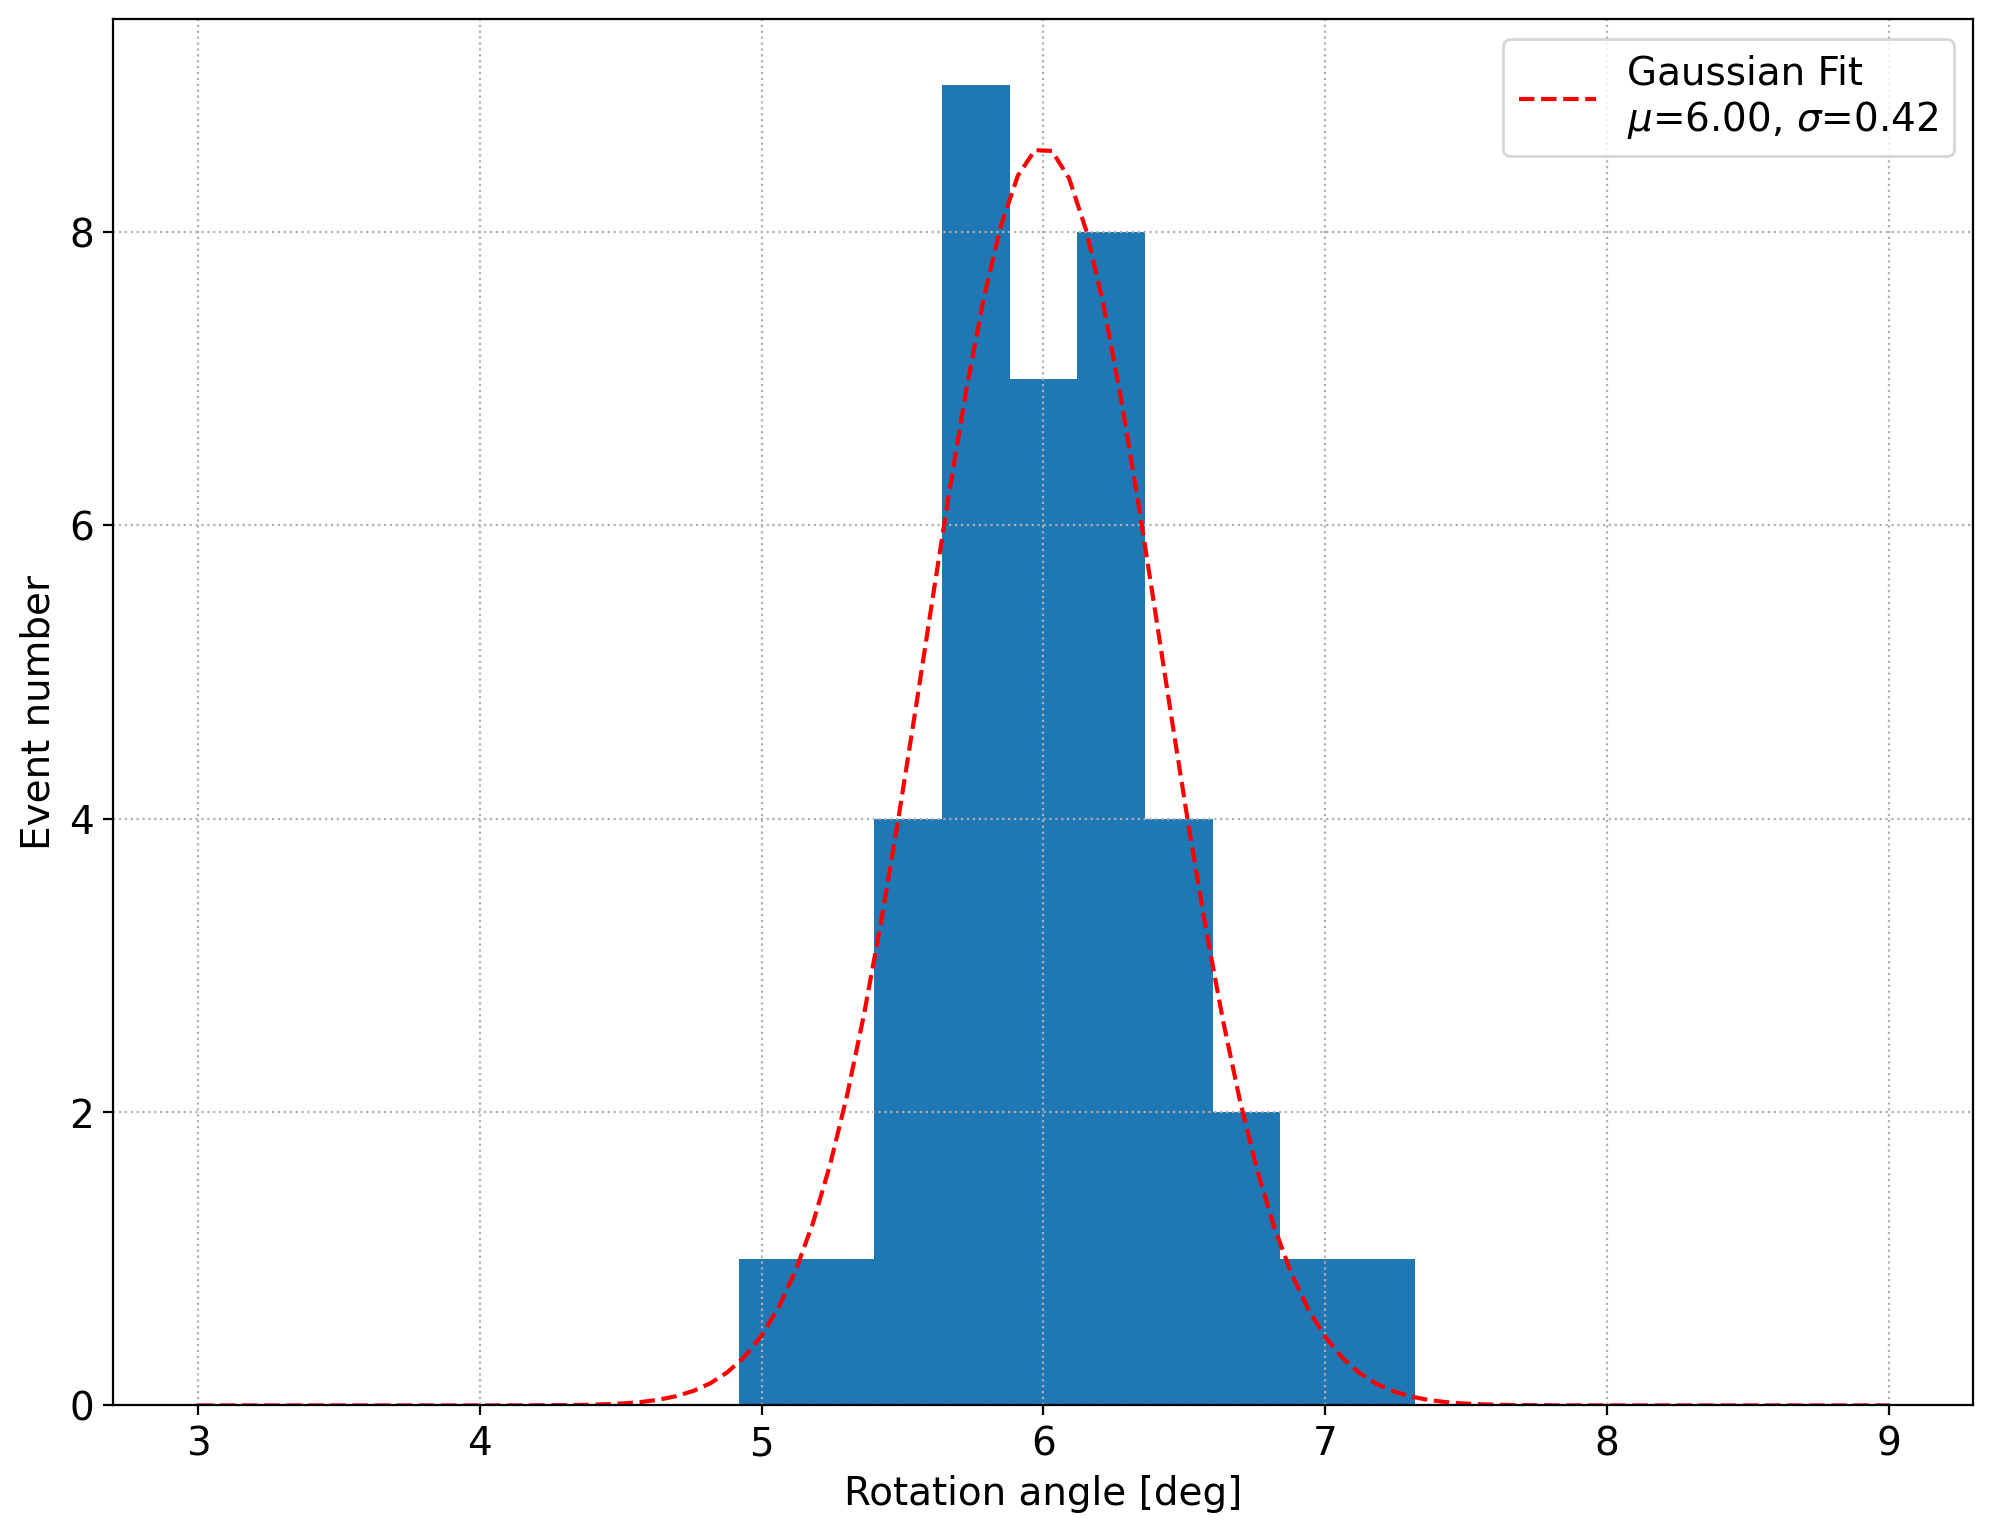
\includegraphics[width=0.8\columnwidth]{5_alignment/figs/hist_rotation_angle2.png}
  \caption{回転角データのガウシアンフィット。}
  \label{gaussian_fit}
\end{figure}
ガウシアンの中心$\mu=\SI{6.00}{^{\circ}}$と分散$\sigma^{2}=0.17$を得た。これより、最終的な回転角を$\SI{6.00}{^{\circ}}$と決定した。

\subsection{回転する上でのジグの必要性}
決定した回転角分だけ望遠鏡を視線方向軸の周りに回転させれば理想とする検出器配置になると考えられるが、回転にあたって望遠鏡の機構上の問題点があった。GroundBIRDの視線方向軸周りの回転機構の概略を図\ref{gb_fixing_system}に示す。
\begin{figure}[htbp]
  \centering
  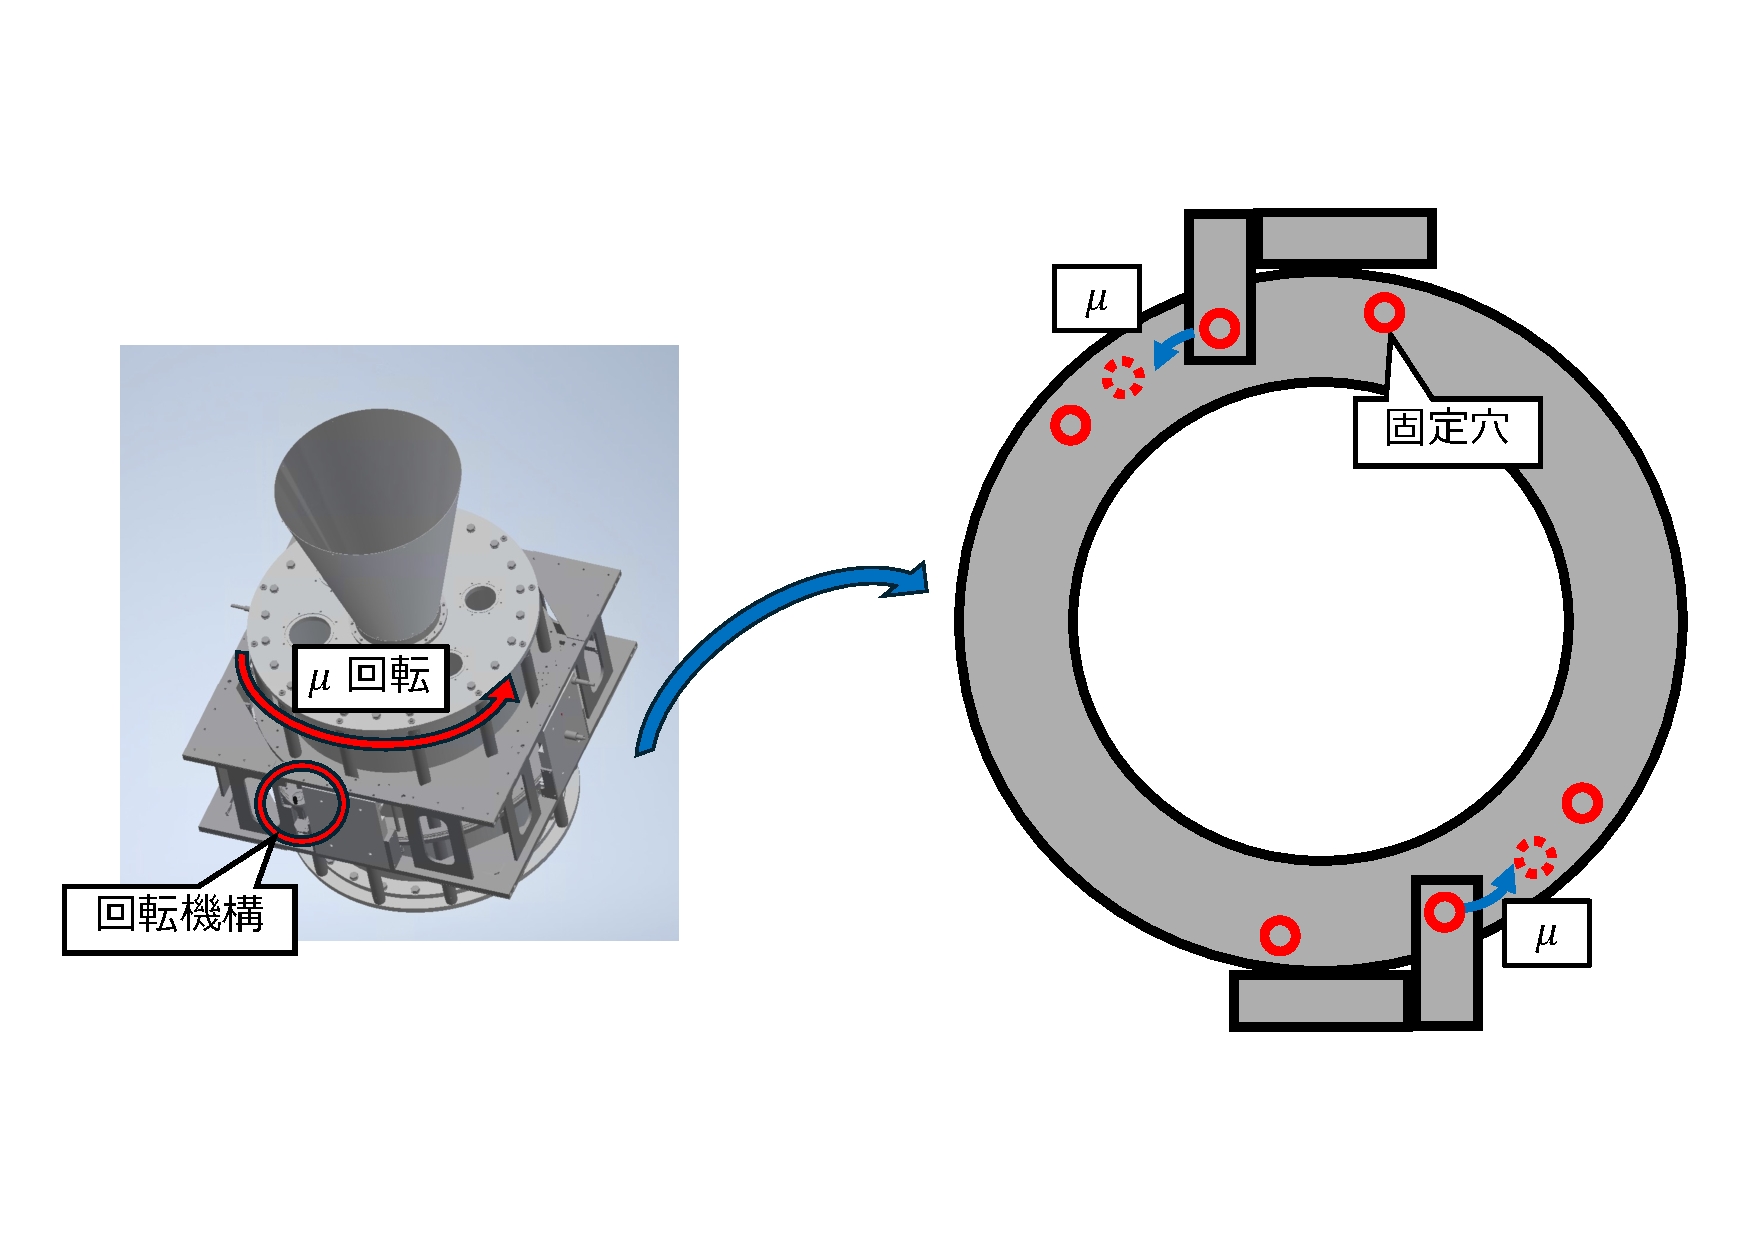
\includegraphics[width=0.85\columnwidth]{5_alignment/figs/gb_fixing_system.pdf}
  \caption{GroundBIRDの視線方向軸周りの回転機構。固定穴の角度間隔に対して理想的なアライメントにするための回転角が小さい。}
  \label{gb_fixing_system}
\end{figure}
望遠鏡クライオスタットが外側の支持部によって支えられているとともに、歯車で視線方向軸周りに回転できるようになっている。また、クライオスタットと支持部は固定穴にネジを締めることで固定されている。しかし、この穴は円周上に等間隔で24箇所しか空けられていない設計になっていた。つまり、$\SI{15}{^{\circ}}$ずつの回転でしか固定ができないようになっていた。そのため、必要な回転角で回転をした後に固定ができず、安全性が担保できないという点で問題だった。

この問題に対処するために、回転後に望遠鏡のクライオスタットと支持部を固定するための機構が必要であり、本論文では固定用のジグを新しく導入することを考えた。
\section{ジグの設計と現地インストール}

\subsection{固定用ジグの作成}
回転後の固定用ジグの設計は回転によって移動する固定穴の距離を基に長さを決めて行った。図\ref{jig_fixing}に設計したジグと望遠鏡内での設置位置を示す。
\begin{figure}[htbp]
  \centering
  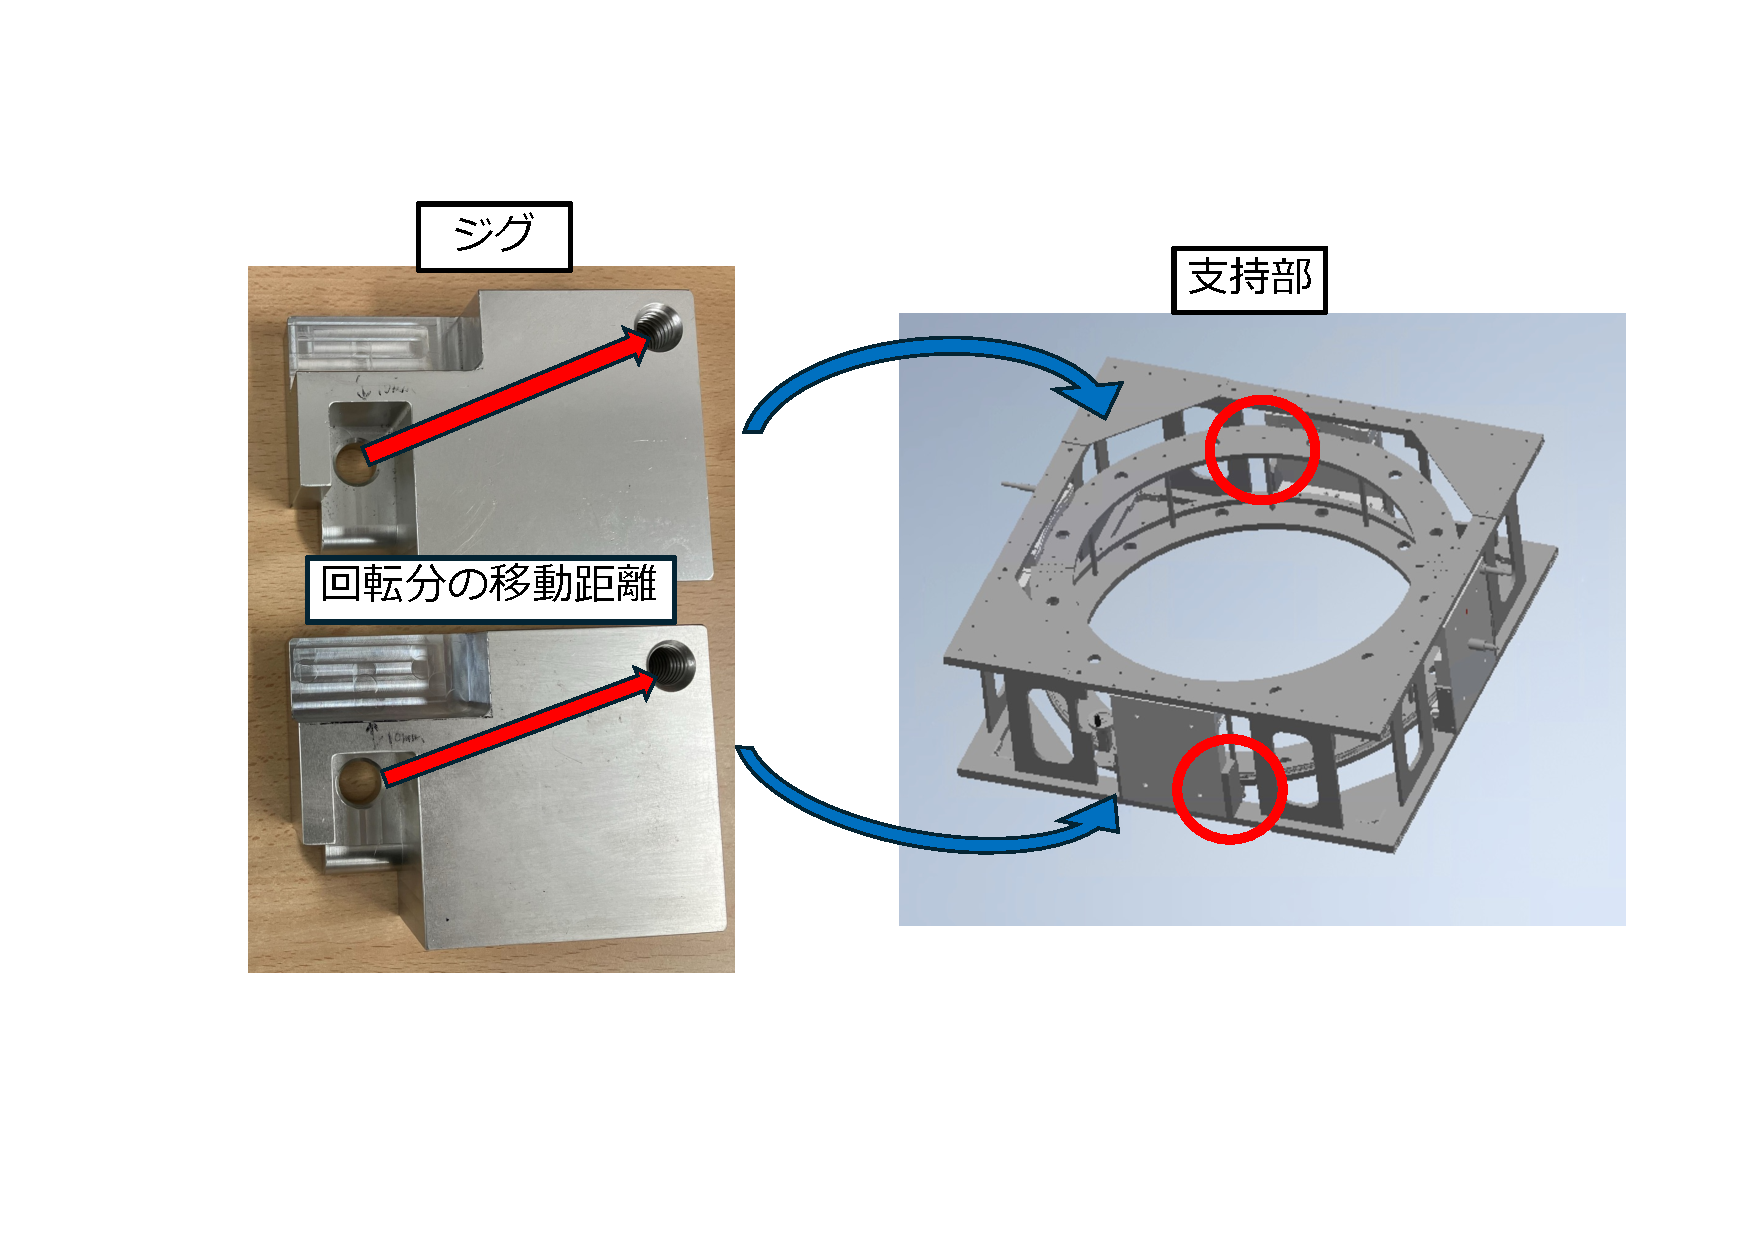
\includegraphics[width=0.85\columnwidth]{5_alignment/figs/jig_making.pdf}
  \caption{設計したジグと望遠鏡支持部への設置位置。固定穴は対角線上に2箇所あるため、それに合わせたジグも2個必要になる。}
  \label{jig_fixing}
\end{figure}
本来の固定穴があった位置と移動した後の固定穴の位置にそれぞれネジで締めるための穴を空けている。また、回転角に対して柔軟な設計にはなっていないため、回転角とジグは1対1対応になっている。回転角の見積もりをジグの設計時には間違えており$\SI{8.25}{^{\circ}}$と試算していた。そのため、ジグの設計も$\SI{8.25}{^{\circ}}$の回転に対応したものになってしまった。以降で述べる実装はこの角度の回転に伴っている。実装後に取得した観測データも$\SI{8.25}{^{\circ}}$回転した検出器配置でのデータになる。その点を考慮していただきたい。

\subsection{望遠鏡への実装}
設計したジグを実際の望遠鏡に実装した(2024/08/29)。望遠鏡を視線方向軸の周りに回転させ、その後設計したジグで固定した。固定後のジグの様子を図\ref{jig_install}に示す。
\begin{figure}[htbp]
  \centering
  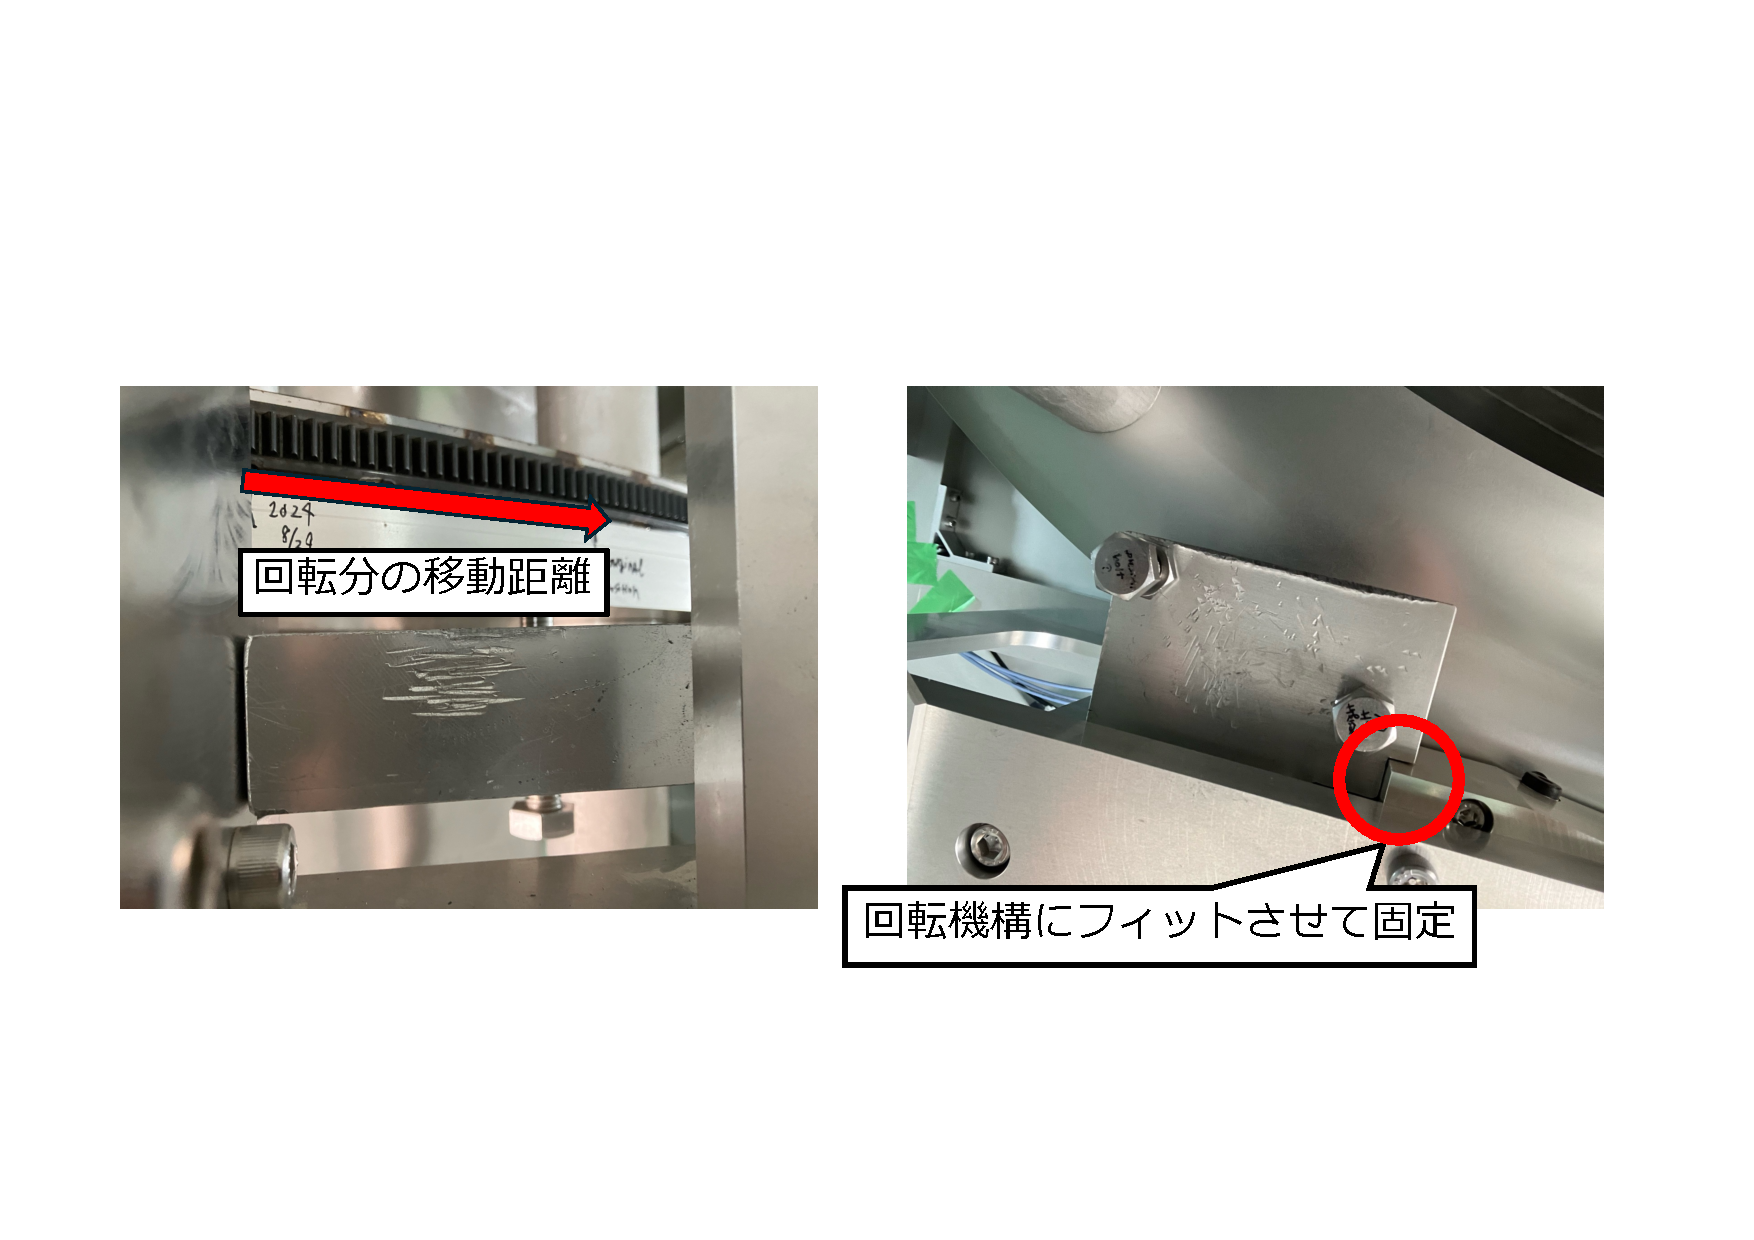
\includegraphics[width=0.85\columnwidth]{5_alignment/figs/jig_install.pdf}
  \caption{視線方向軸周りの回転後にジグで固定した望遠鏡支持部とクライオスタット。}
  \label{jig_install}
\end{figure}
ジグは望遠鏡支持部の回転機構に対してフィットするように設計してあるため、固定の強度は十分である。固定後は安全性の確認のために、望遠鏡の方位角回転をさせて稼働に問題がないかをモニターした。連続運転を行なっても異常がないことを確認し、観測を再開させた。実装後に取得したデータは本来の検出器配置に対して$\SI{8.25}{^{\circ}}$回転させたもので、\ref{angle_calculation}で求めた理想とする回転角$\SI{6.00}{^{\circ}}$より$\SI{2.25}{^{\circ}}$余分に回転させた配置となっている。つまり、理想とする最適な配置ではないが、従来に比べてスキャン軸により沿った配置に是正されていることになる。

\section{天体を用いた較正結果の確認}

\subsection{月データによる確認}
\label{moon_ana}
視線方向軸周りによる検出器配置の変化を\ref{angle_calculation}と同様にして月の観測データから確認した。使用した観測データを表\ref{after_full_array_table}に示す。
\begin{table}[htbp]
  \centering
  \caption{ビーム中心マップの構成に使用した月観測データ(回転後)}
  \vspace{3mm}
  \begin{tabular}{cccc} \hline
    観測日(UTC) & 観測時間 [min] & 周波数 [GHz] & 月の昇降(rise or set) \\ \hline
    2024/08/30 7:56 - 8:56 & 60 & 145 & rise \\
    2024/08/30 8:12 - 9:12 & 60 & 145 & rise \\
    2024/08/30 8:19 - 9:19 & 60 & 145 & rise \\
    2024/08/30 8:26 - 9:26 & 60 & 220 & rise \\
    2024/08/30 8:42 - 9:42 & 60 & 145 & rise \\
    2024/08/30 8:54 - 9:54 & 60 & 145 & rise \\ \hline

  \end{tabular}
  \label{after_full_array_table}
\end{table}
ここで、\SI{145}{GHz}アレイの1つはDAQの不調により、データを取得できなかった。これらのデータを使って再構成したビーム中心マップを図\ref{after_full_beam_map}に示す。

\begin{figure}[htbp]
  \centering
  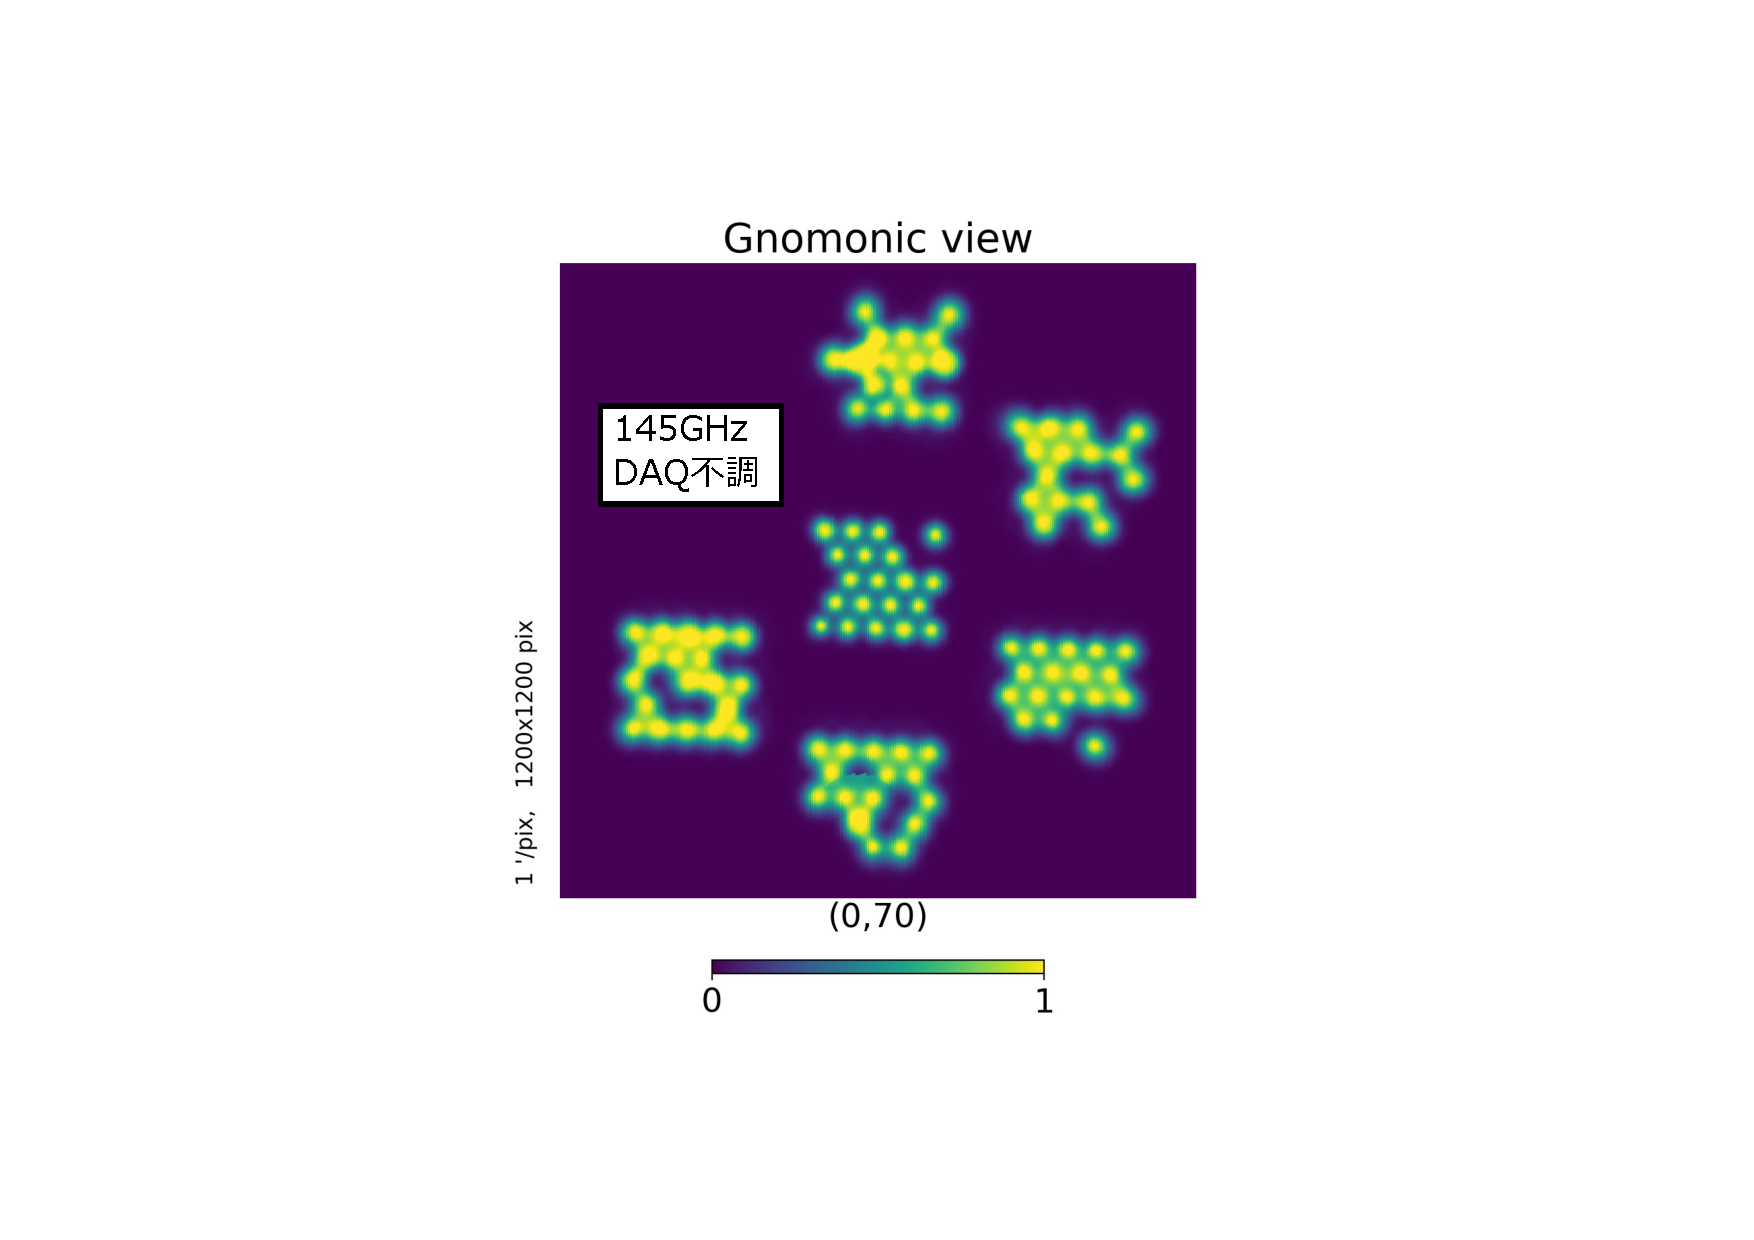
\includegraphics[width=0.8\columnwidth]{5_alignment/figs/after_full_gnomonic_70_mod.pdf}
  \caption{視線方向軸周りの回転後のビーム中心マップ。}
  \label{after_full_beam_map}
\end{figure}
回転前の図\ref{before_full_beam_map}と比較することで検出器の配置がスキャン軸に沿った方向へとビーム中心に対して回転したことが見て取れる。この図はあくまで仰角$\SI{70}{^{\circ}}$中心の配置を平面射影したもので、位相の最大点をとった視線を仰角$\SI{0}{^{\circ}}$の球面で見たもの(図\ref{after_full_pos_0})に対応している。これを実際の仰角$\SI{70}{^{\circ}}$での球面での視線で見ると図\ref{after_full_pos_70}のようになる。
\begin{figure}[htbp]
  \centering
  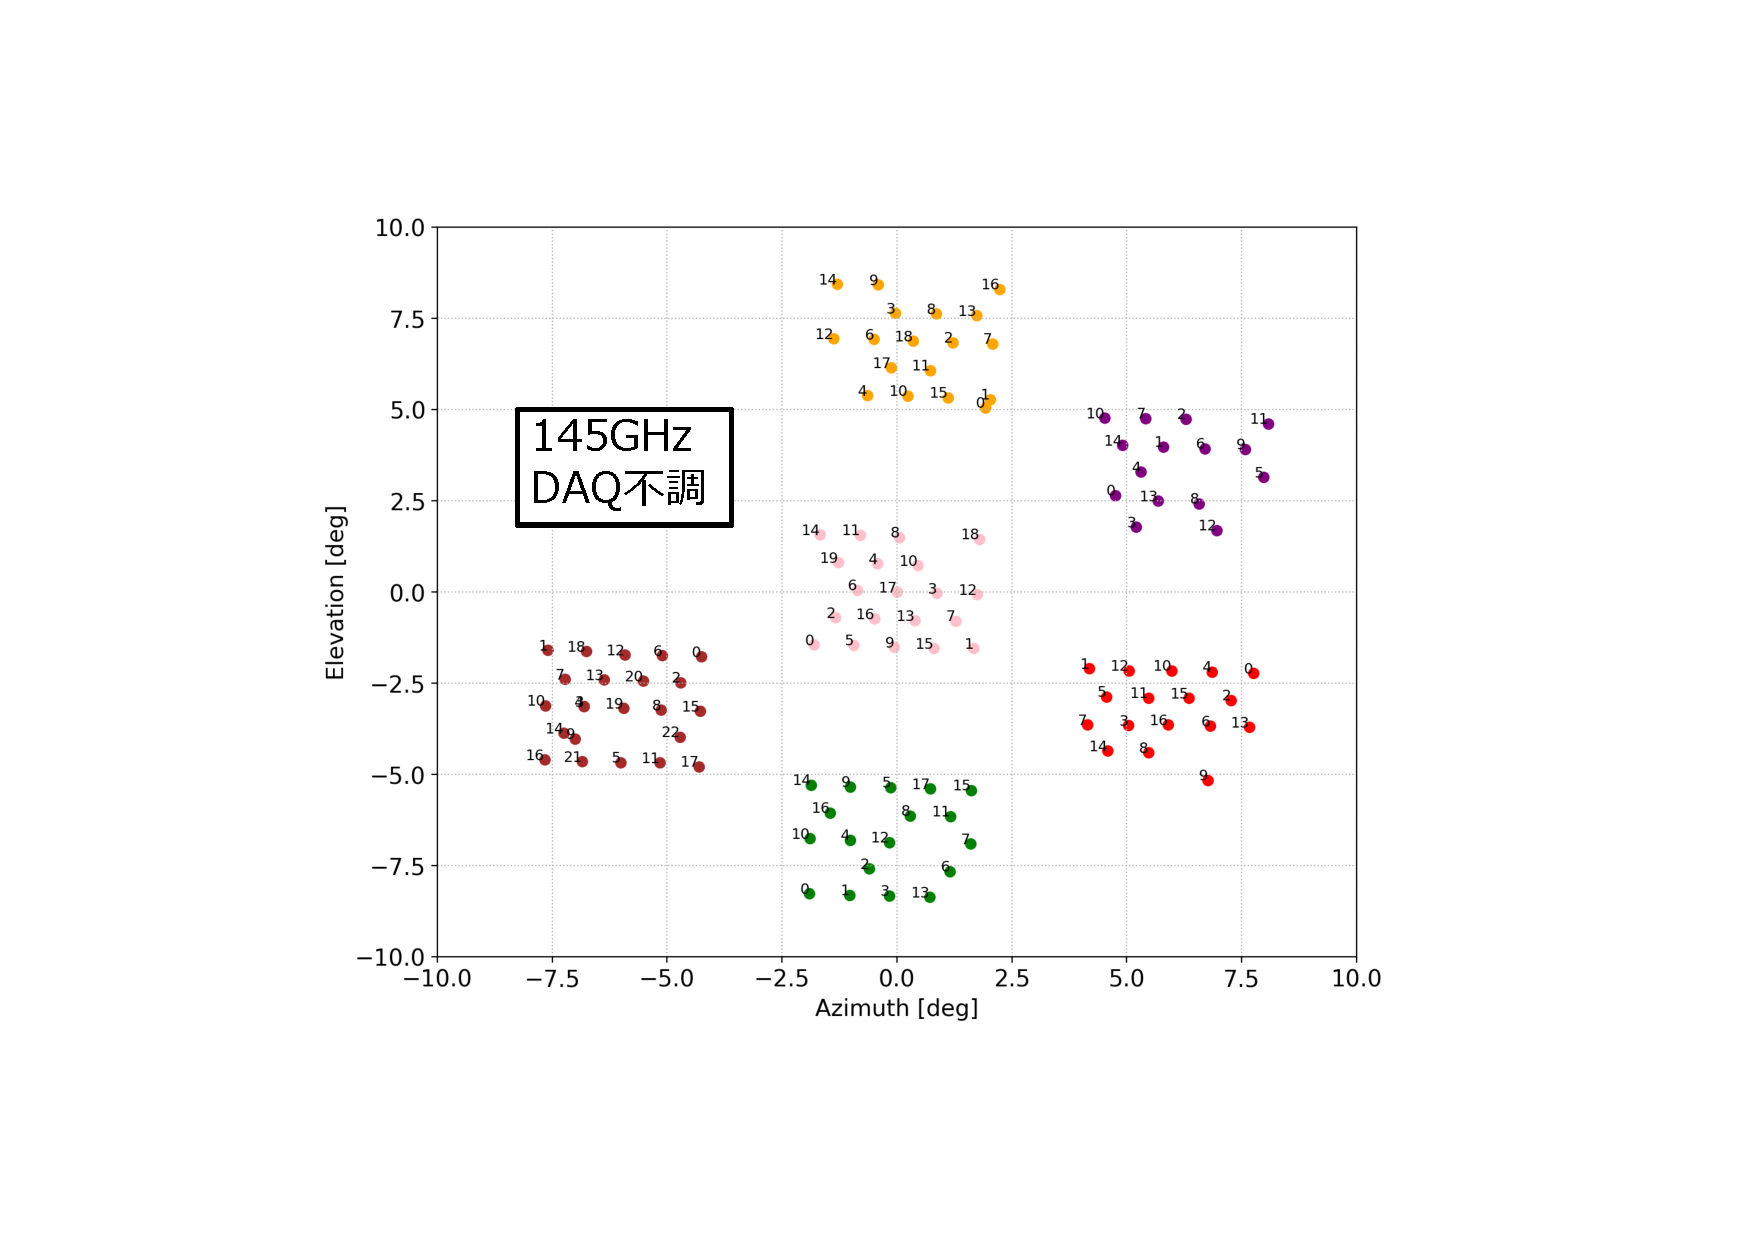
\includegraphics[width=1.0\columnwidth]{5_alignment/figs/after_full_pos_0_mod.pdf}
  \caption{座標変換により平面的に見た回転後のビーム中心の視線。}
  \label{after_full_pos_0}
\end{figure}
\begin{figure}[htbp]
  \centering
  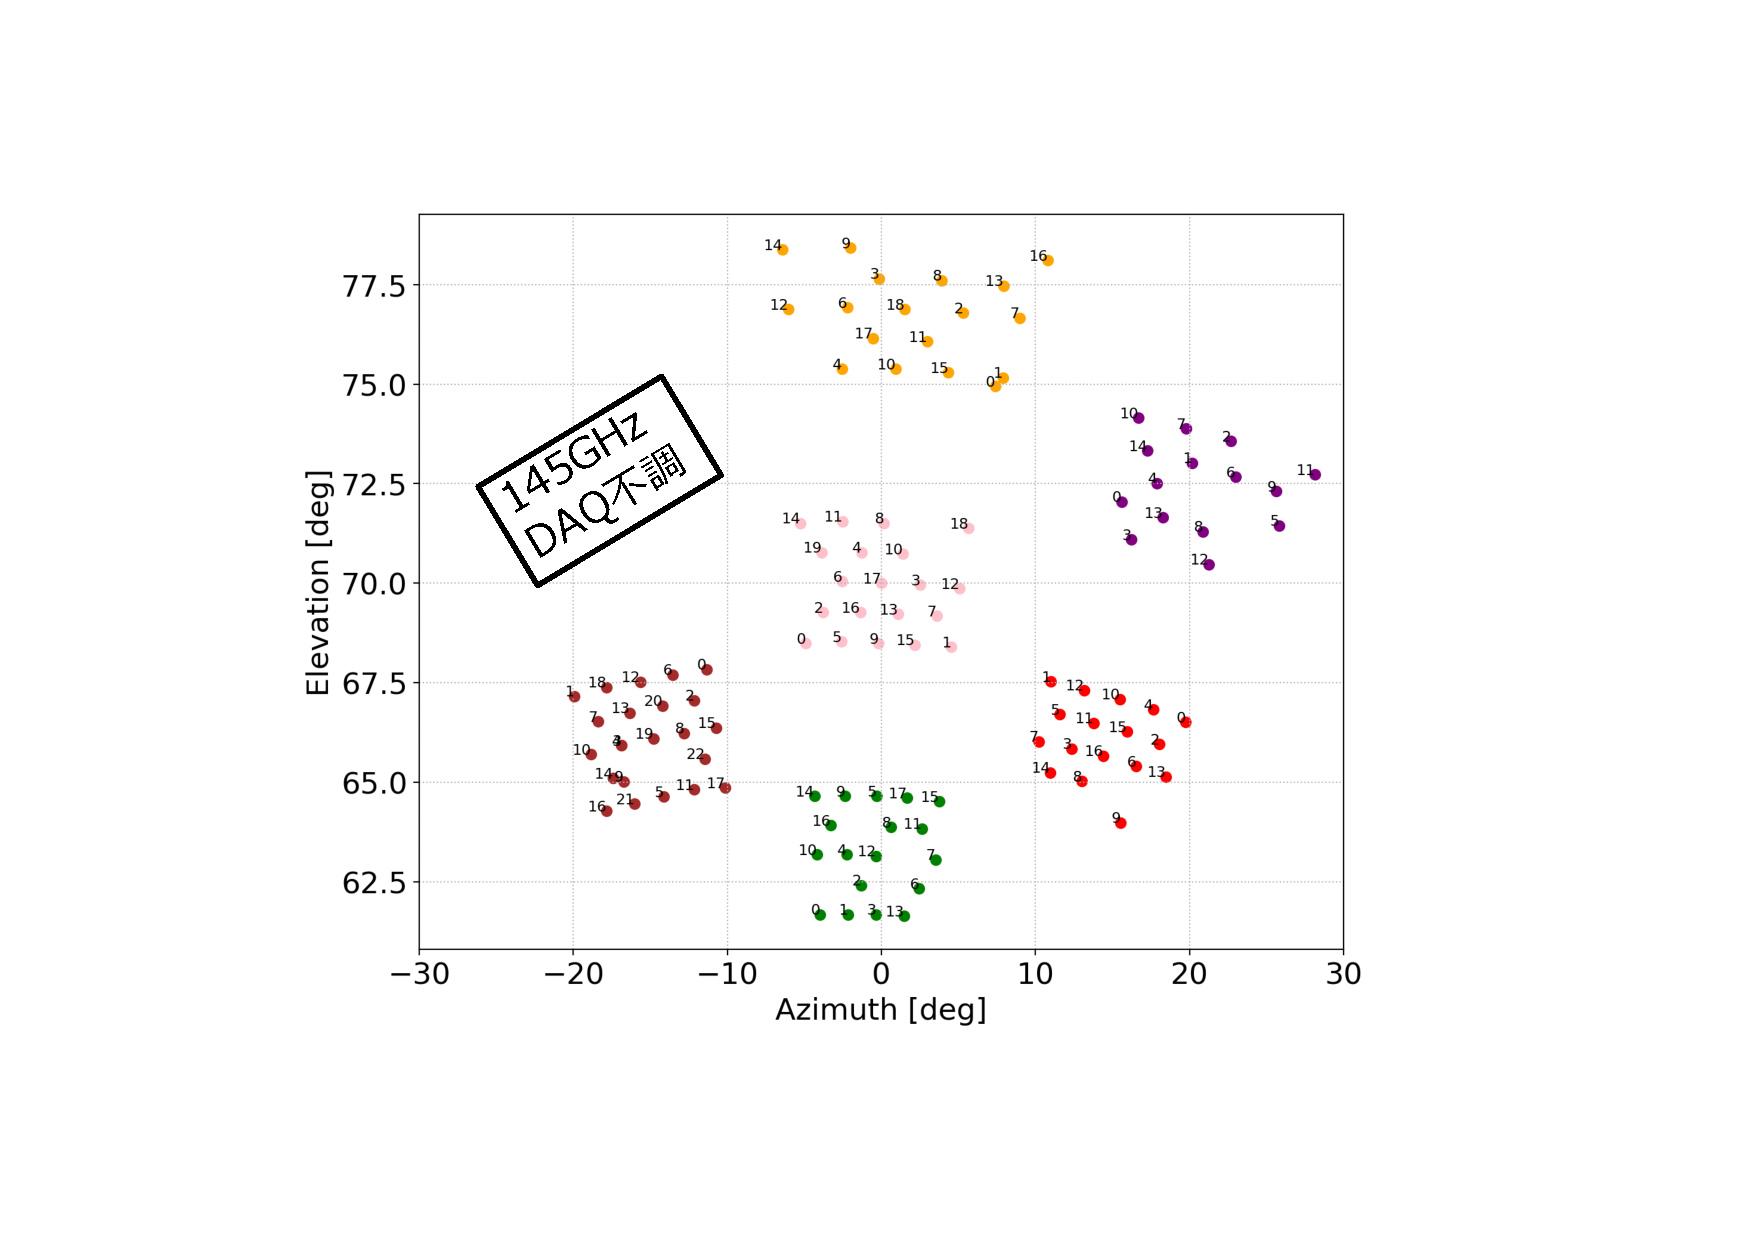
\includegraphics[width=1.0\columnwidth]{5_alignment/figs/after_full_pos_70_mod.pdf}
  \caption{回転後の全検出器の視線。球面による歪みによって生じる非対称性が回転によって是正された。}
  \label{after_full_pos_70}
\end{figure}
図\ref{before_full_beam_pos}では検出器の配置が傾いていることに加えて、球面による歪みの効果によって特に\SI{145}{GHz}アレイでビーム中心に対する非対称性が見られた。視線方向軸周りの回転でこの非対称性は大きく補正されたことが分かる。一方で余分に回転させたことによる傾きが残っていることも見て取れる(図\ref{10960_beam_centered})。しかし、図\ref{before_full_beam_pos}と図\ref{after_full_pos_70}との比較で分かるように、全検出器としての視線はスキャン軸に対する角度の傾きに歪みの効果が加わるため、回転による較正で配置は大きく改善された結果となった。
\begin{figure}[h]
  \begin{tabular}{cc}
    %---- 最初の図 ---------------------------
    \begin{minipage}[t]{0.48\hsize}
      \centering
      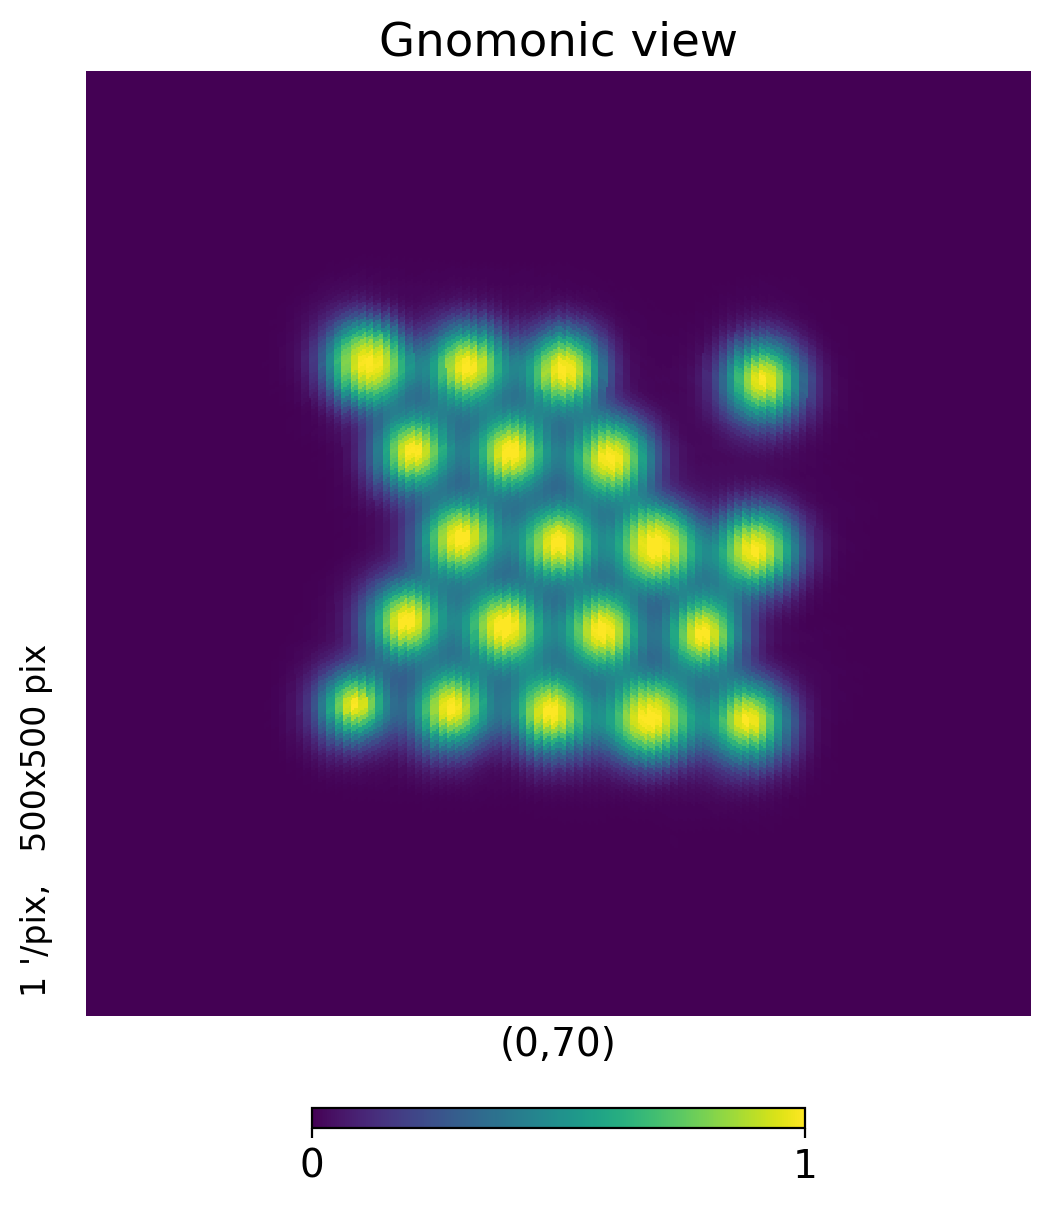
\includegraphics[keepaspectratio, scale=0.4]{5_alignment/figs/10960_gnomonic.png}
      \subcaption{\SI{220}{GHz}アレイのビーム中心マップ。}
      \label{10960_gnomview}
    \end{minipage}
    %---- 2番目の図 --------------------------
    \begin{minipage}[t]{0.48\hsize}
      \centering
      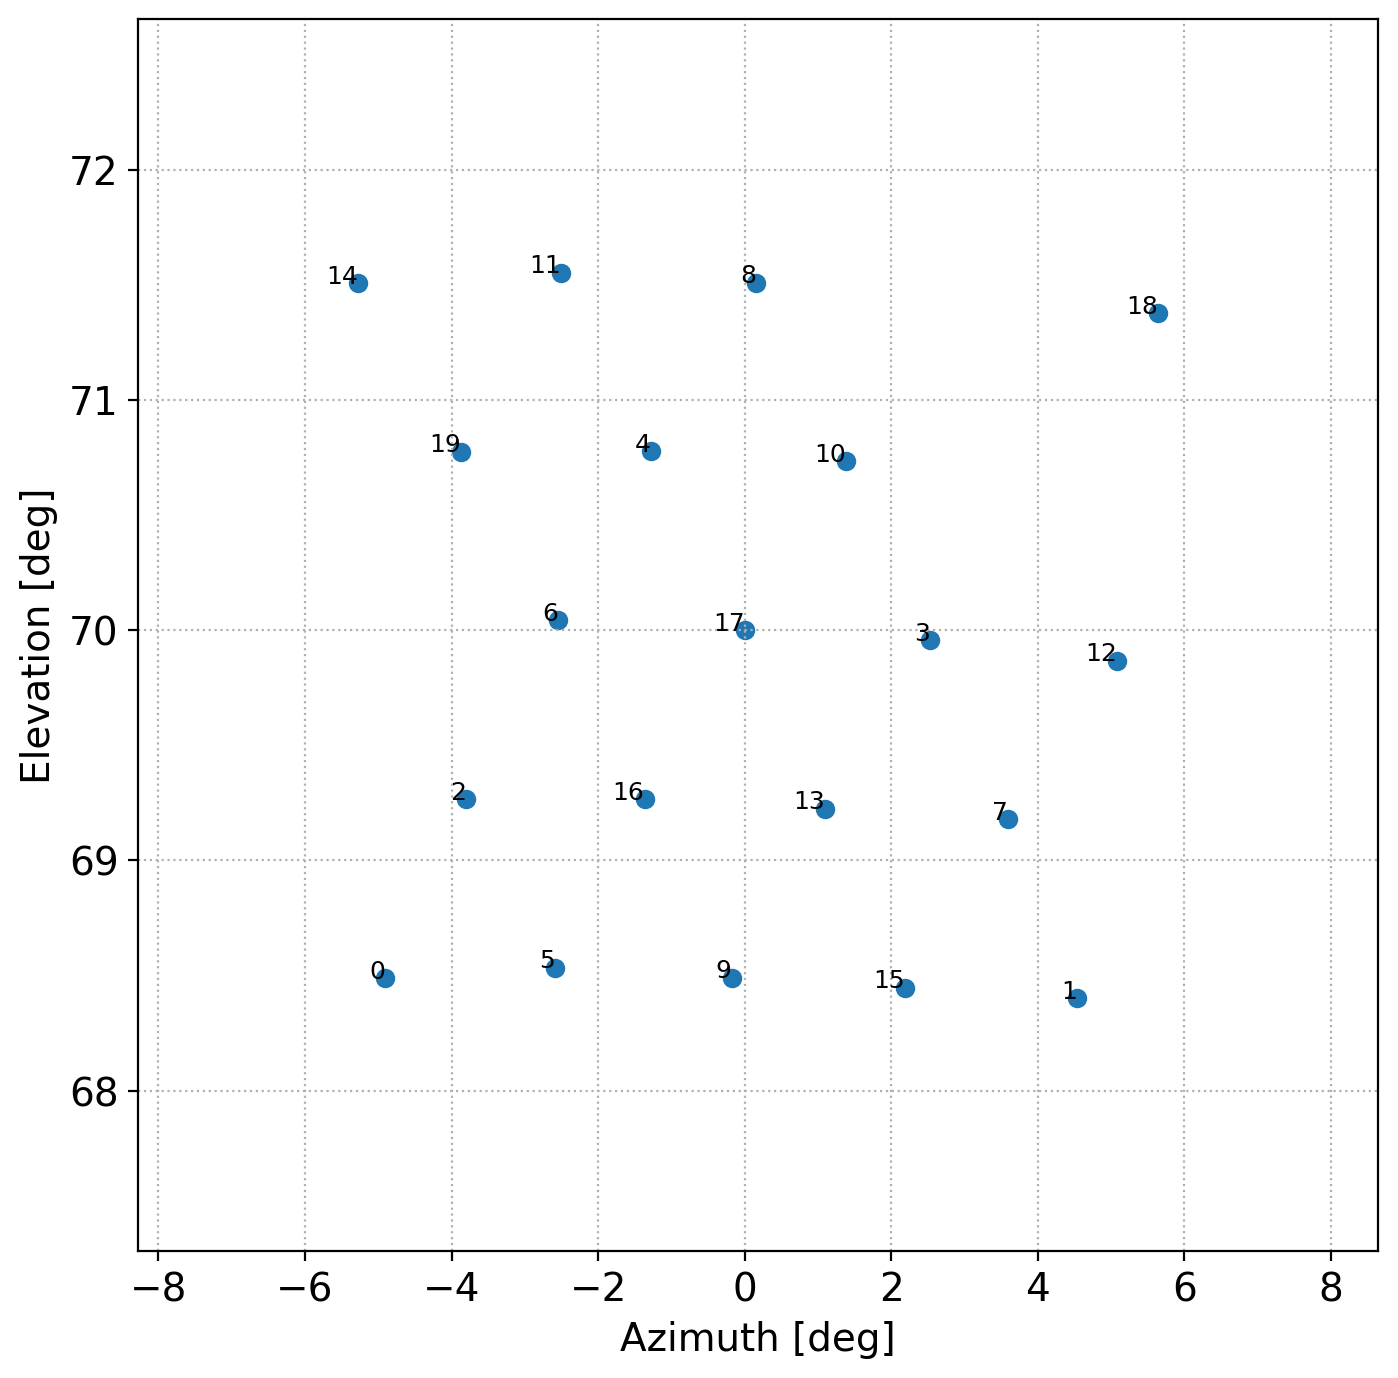
\includegraphics[keepaspectratio, scale=0.32]{5_alignment/figs/10960_pos_kid17_70.png}
      \subcaption{各検出器のビーム中心の視線。}
      \label{10960_pos}
    \end{minipage}
    %---- 図はここまで ----------------------
  \end{tabular}
  \caption{ビーム中心マップから取得した検出器の視線(\SI{220}{GHz}、回転後)。中心アレイでは歪みの影響が少ない分、余分に回転させたことによるスキャン軸に対する傾きが残っていることが見て取れる。}
  \label{10960_beam_centered}
\end{figure}

\subsection{木星データによる確認}
\label{jupiter_ana}
次に\ref{moon_ana}で見た検出器アライメントの較正結果を木星の観測データでも確認した。木星は表\ref{moon_vs_planet}にまとめたように点源として扱えるため検出器の視線を知る上ではより正確であるが、信号が小さくノイズに埋もれやすいため、月より観測は難しい。そのため、月での結果を再現して較正結果の妥当性を保証することを目的として行った。以下では\SI{220}{GHz}アレイでの結果のみを述べる。木星は望遠鏡のビーム幅に対してその角直径は十分小さい。この場合、木星観測時のアンテナ温度$T_{\mathrm{Jupiter}}$は
\begin{equation}
  T_{\mathrm{Jupiter}}=\frac{\overline{T_{\mathrm{B}}}\Omega_{\mathrm{Jupiter}}}{\Omega_{\mathrm{A}}}
\end{equation}
と表せる。ここで、$\Omega_{\mathrm{A}}$はビーム立体角、$\Omega_{\mathrm{Jupiter}}$は木星のビームの広がり、$\overline{T_{\mathrm{B}}}$は、木星の平均輝度温度である。つまり、真の木星輝度温度よりも観測されるアンテナ温度は十分小さくなる。木星の輝度温度は周波数依存性があるが、ミリ波帯での典型的な値\SI{150}{K}とし、木星の角直径$\sim\SI{40}{''}$、\SI{220}{GHz}検出器のビーム幅\SI{25}{'}からアンテナ温度を見積もると、おそよ$T_{\mathrm{Jupiter}}\sim$\SI{100}{mK}と小さいことが分かる。実際、木星観測時のTODを見るとノイズに信号が埋もれて木星のマップを再構成できないことがある。TODには大気放射に由来するノイズが混入し、それは大気中の水蒸気量が多い時ほど顕著になって木星由来の信号の邪魔となる。そのため、木星の観測データの中でも十分PWVが小さいものを主な解析対象とした。また、木星中心座標データから以下の処理
\begin{enumerate}
  \item スキャンごとの位相を線形関数でフィットし、ベースラインを差っ引く
  \item $\SI{0.2}{^{\circ}}\cdot\SI{0.2}{^{\circ}}$の角度領域でリビンし、領域内の位相の平均をとり、その値を代表値とする
\end{enumerate}
を行なった。まず、PWVが比較的高い観測のTODと各検出器の木星中心マップを図\ref{5862_jupiter}に示す。
\begin{figure}[htbp]
  \centering
  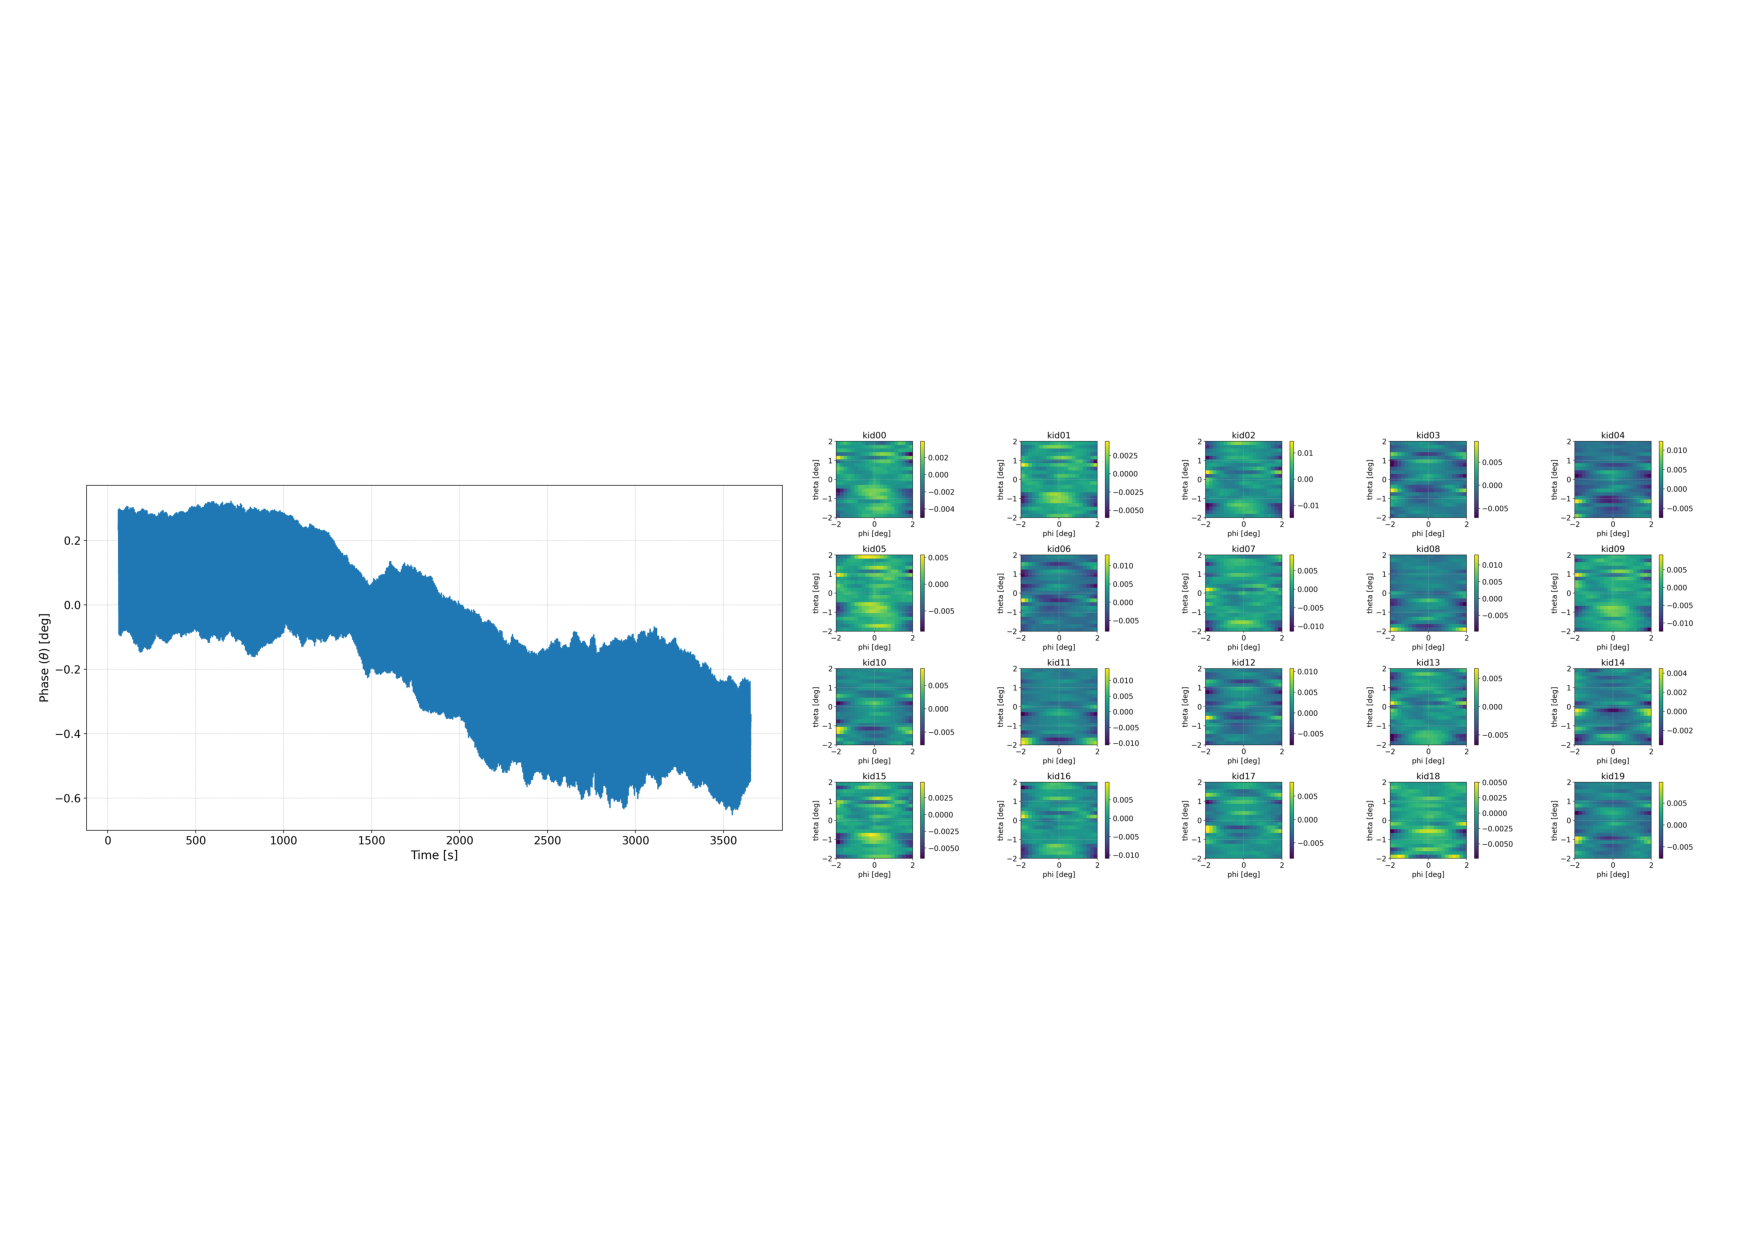
\includegraphics[width=1.0\columnwidth]{5_alignment/figs/5862_jupiter.pdf}
  \caption{高いPWVでの木星観測データ(2023/07/27, PWV= \SI{4.6}{mm})。(左)1観測でのTOD。(右)ベースラインを引き、リビンした後の木星中心マップ。}
  \label{5862_jupiter}
\end{figure}
ここで、PWVの値はTODの観測時間内のPWVデータベースの平均値をとっている。月中心マップ(図\ref{moon_centered_6550})では中心に月のマップが鮮明に見えたが、この木星データでは木星のマップが見て取れない。

次にPWVが十分低い観測での木星中心データを図\ref{5987_jupiter}に示す。
\begin{figure}[htbp]
  \centering
  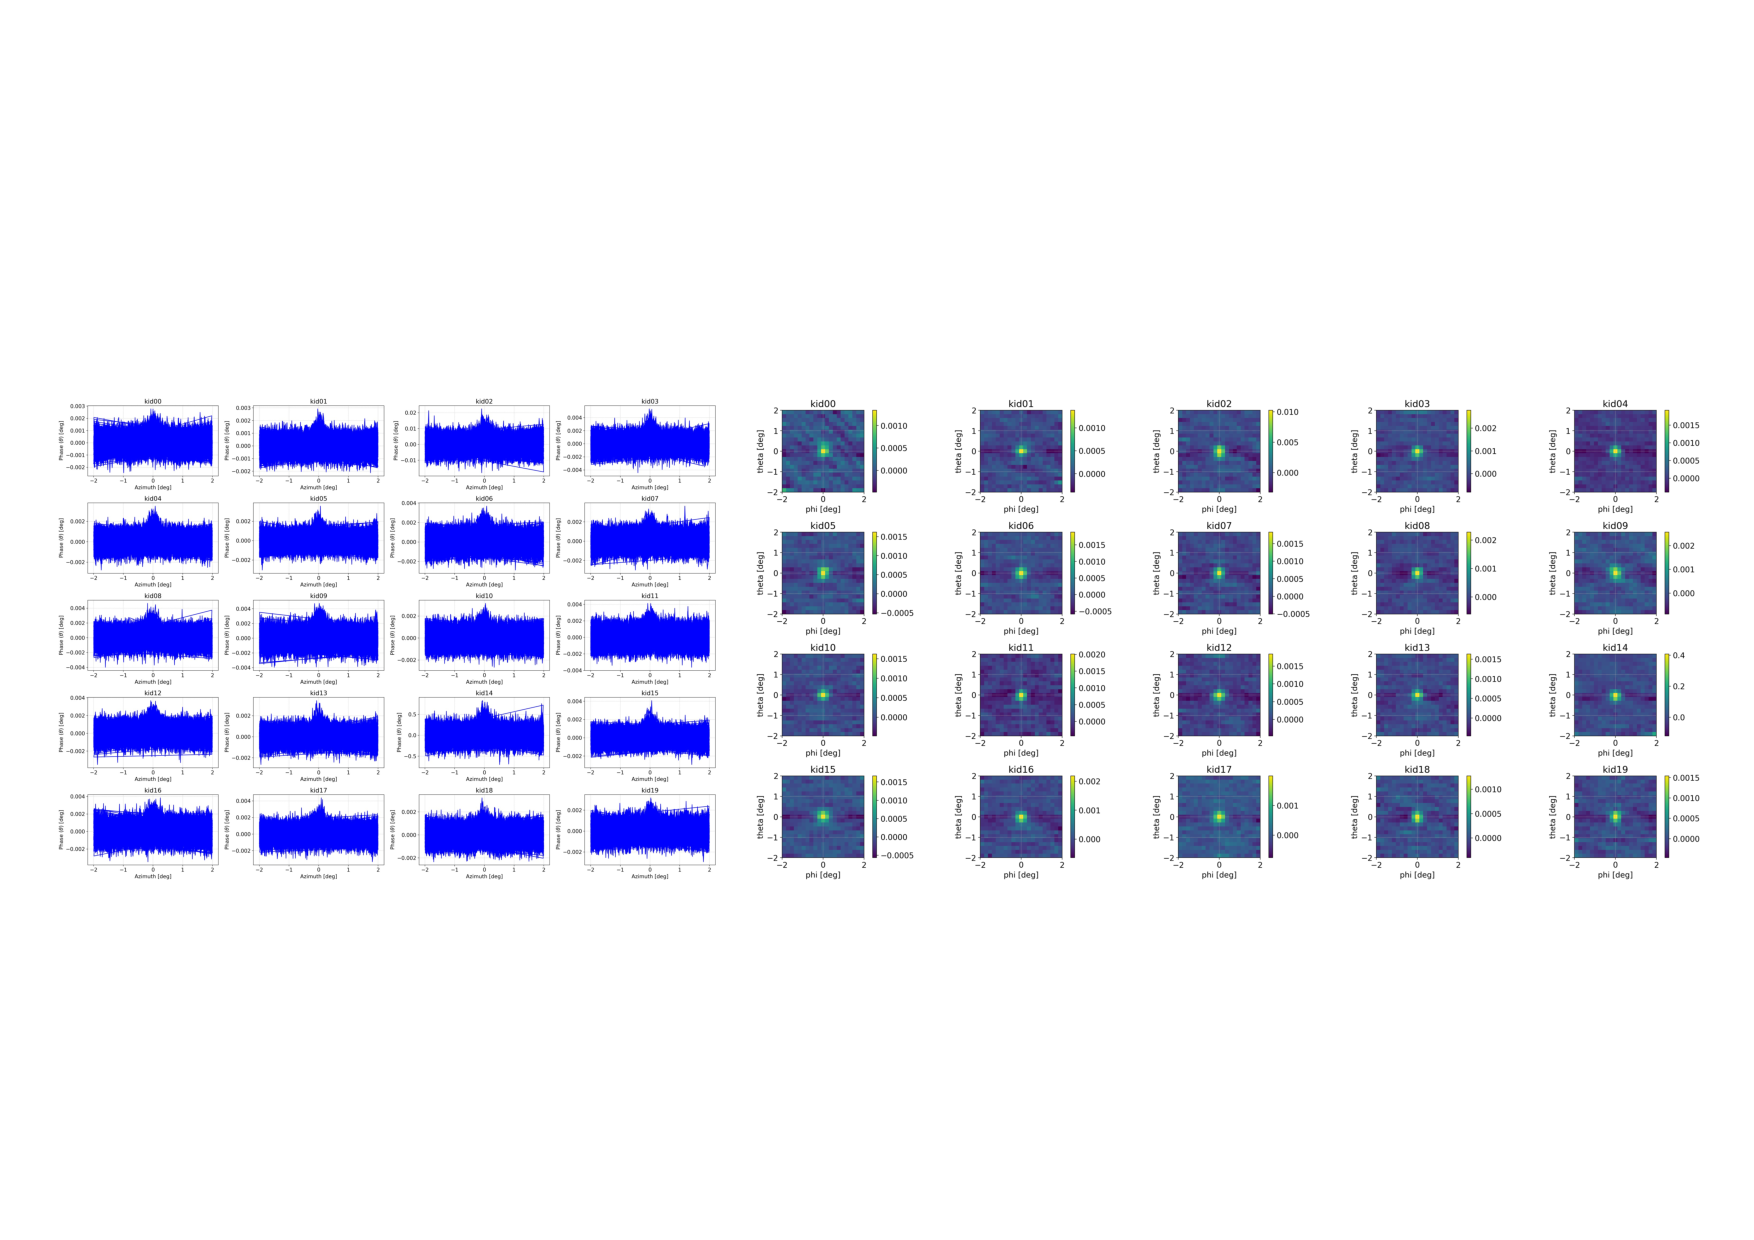
\includegraphics[width=1.0\columnwidth]{5_alignment/figs/5987_jupiter.pdf}
  \caption{十分低いPWVでの木星観測データ(2023/07/28, PWV= \SI{0.83}{mm})。(左)ベースラインを引いた後の木星中心座標での位相。中心付近で位相が高くなっており、これが木星の信号に対応している。(右)ベースラインを引き、リビンした後の木星中心マップ。}
  \label{5987_jupiter}
\end{figure}
月と同様にして鮮明な木星のマップを得られた。これより、十分PWVが低く観測条件が整っていれば1時間のTODで木星を観測できることが分かった。一方でPWVが比較的高い時は1観測では木星を見ることはできず、データを蓄積する必要がある\footnote{十分にPWVが低く、かつ木星が通過する時間での観測データは現在時点では数観測しか確認できていない。そのため、十分ではないが比較的低いPWVでの観測データを蓄積し、S/N比を上げて木星を見るような解析手法が求められる。}。

得られた木星中心マップから月と同様にして、各検出器の視線を求めた。視線方向軸周りの回転前のものを図\ref{5987_jupiter_pos}に、回転後のものを図\ref{11280_jupiter_pos}に示す。
\begin{figure}[htbp]
  \centering
  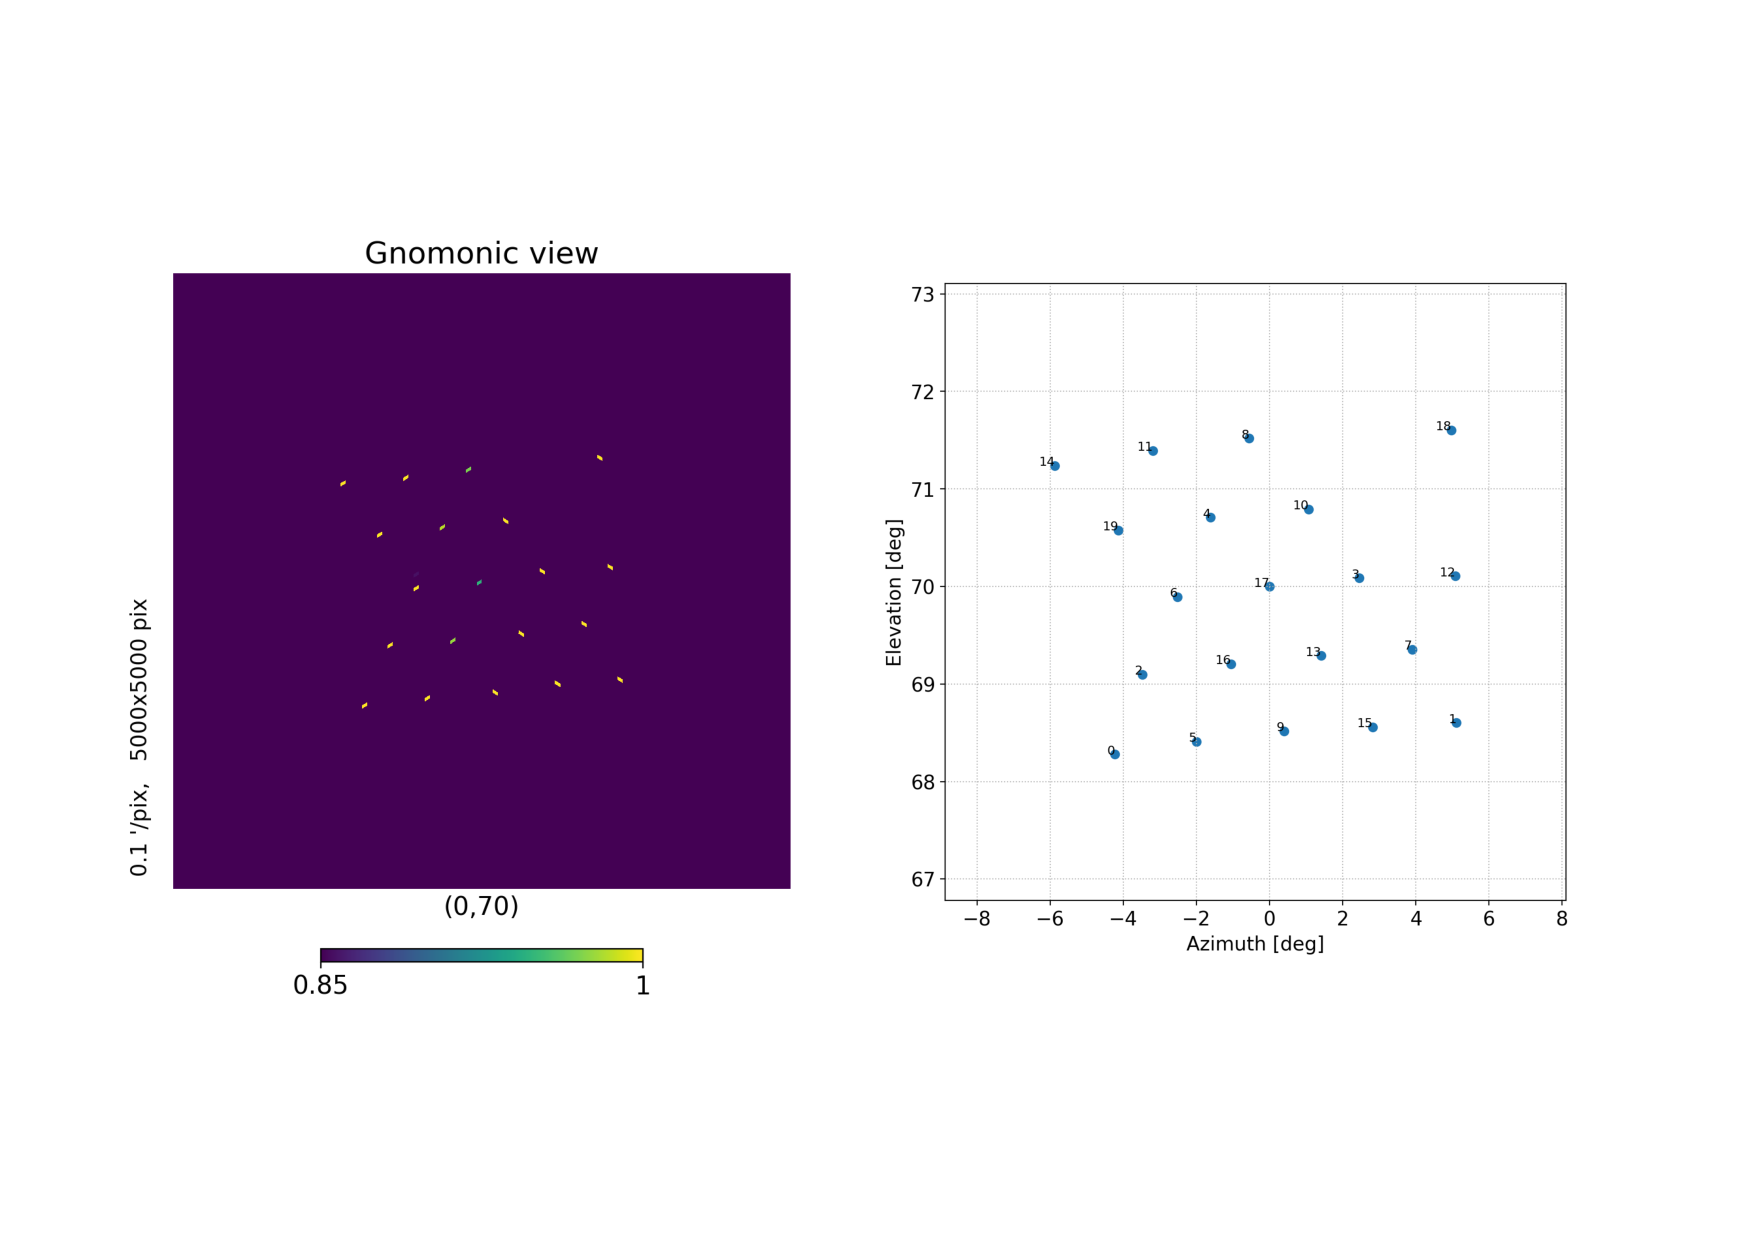
\includegraphics[width=1.0\columnwidth]{5_alignment/figs/5987_jupiter_pos.pdf}
  \caption{木星データから取得した検出器の視線(回転前、2023/07/28, PWV= \SI{0.83}{mm})。(左)\SI{220}{GHz}アレイのビーム中心マップ。月と比べて信号の広がりが小さい。(右)各検出器のビーム中心の視線。}
  \label{5987_jupiter_pos}
\end{figure}
\begin{figure}[htbp]
  \centering
  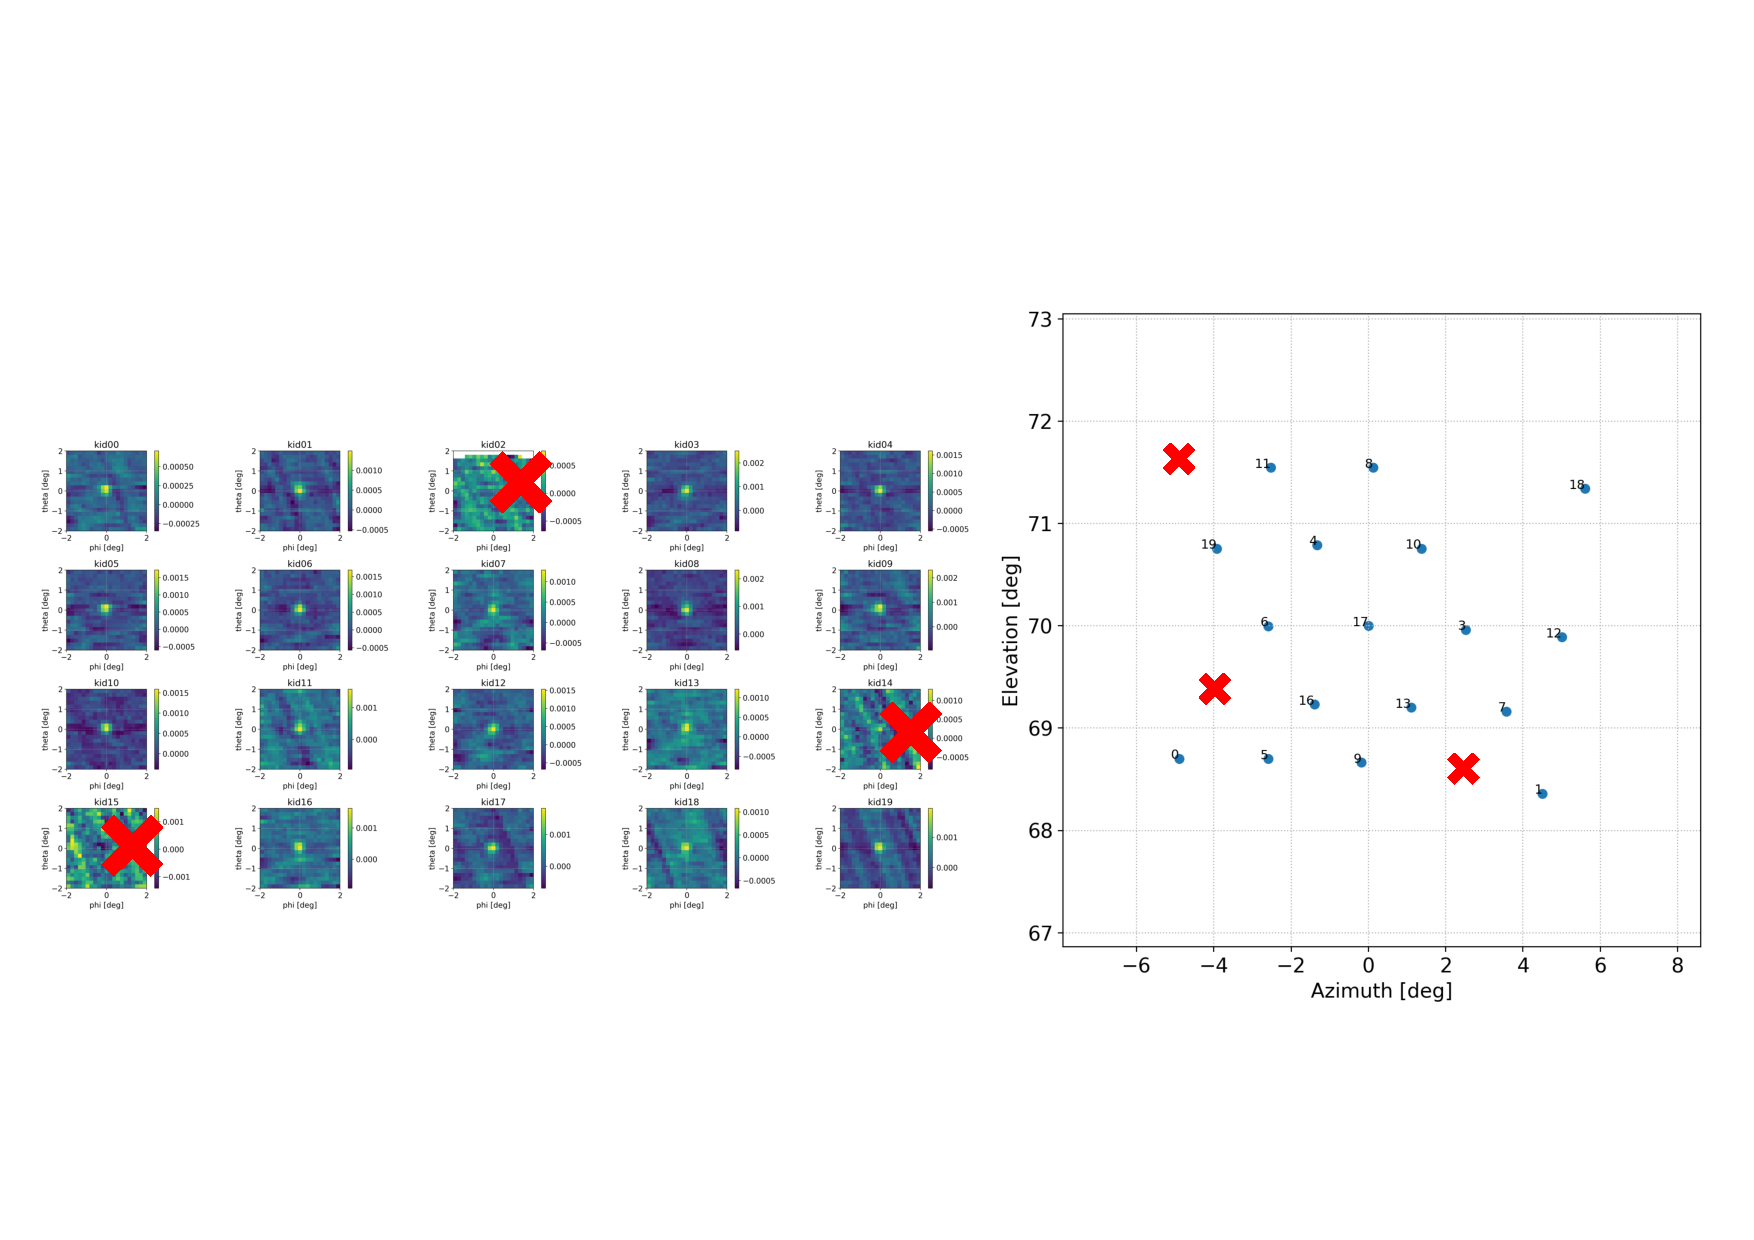
\includegraphics[width=1.0\columnwidth]{5_alignment/figs/11280_jupiter.pdf}
  \caption{木星データから取得した検出器の視線(回転後、2024/09/05, PWV= \SI{0.81}{mm})。(左)\SI{220}{GHz}アレイの各検出器の木星中心マップ。一部の検出器では木星のマップを再構成できていない。(右)各検出器のビーム中心の視線。}
  \label{11280_jupiter_pos}
\end{figure}
回転前と回転後とで、スキャン軸に対する検出器配置の傾きを再現でき、月での結果の妥当性を示している。一方で、回転後の十分低いPWVの観測データでも一部の検出器がノイズに埋もれてしまい、全検出器の視線を取得できなかった。

\section{検出器間差分で見る大気揺らぎの抑制}

\subsection{TODの差分とPSD}
天体の観測データを用いて検出器の配置が回転し、スキャン軸に沿った向きへと較正されたことを見たが、\ref{scan_pair_diff}で述べたように検出器間での信号の差分をとり、同じ大気をスキャンできるようになっているかを確認して初めて理想とする検出器アライメントに近づいたと言える。異なる検出器がスキャンする大気が同じであれば観測するTODは強い相関を持つことに対応する。そのため、この章ではスキャン軸に沿って並ぶ異なる2つの検出器のTOD相関が配置の回転によってどう変化したのか、に着目する。また、球面による歪みの影響が少なく、大気放射の寄与も大きい中心の\SI{220}{GHz}アレイに焦点を置いて議論する。使用したTODを表\ref{pair_diff_table}に示す。
\begin{table}[htbp]
  \centering
  \caption{検出器間差分に使用した\SI{220}{GHz}アレイ観測データ}
  \vspace{3mm}
  \begin{tabular}{cccccc} \hline
    観測日(UTC) & 観測時間 [min] & 観測対象 & 検出器配置 & スキャン & PWV [mm]\\ \hline
    2024/07/01 5:48 - 6:48 & 60 & sky & 回転前 & 9RPM & 0.96\\ \hline
    2024/09/03 17:49 - 18:49 & 60 & sky & 回転後 & 9RPM & 1.1 \\ \hline

  \end{tabular}
  \label{pair_diff_table}
\end{table}
視線方向軸周りの回転を行った前後でPWVの低く、条件が近い観測データを選択した。また、大気放射ノイズを見るために1時間のTODの中で月や木星といった光源となる天体を観測しなかったものを選択した(表中では観測対象が天体ではなく大気なのでskyとした)。

次に同じアレイ内の検出器TODの性質を見ていく。1アレイ内の検出器が観測する空の領域は同じではないが、ある程度狭い角度領域で収まっているため観測する大気もある程度は近いものである。それは検出器配置を回転させる前でも言えることである。そのため、検出器のTODが共通したトレンドを持ち、相関を持つ\footnote{見ている空の領域が近いことによるものと、1アレイで読み出しを行なっていることによる生のTOD以外の要因もあると思われる。}。
\begin{figure}[htbp]
  \centering
  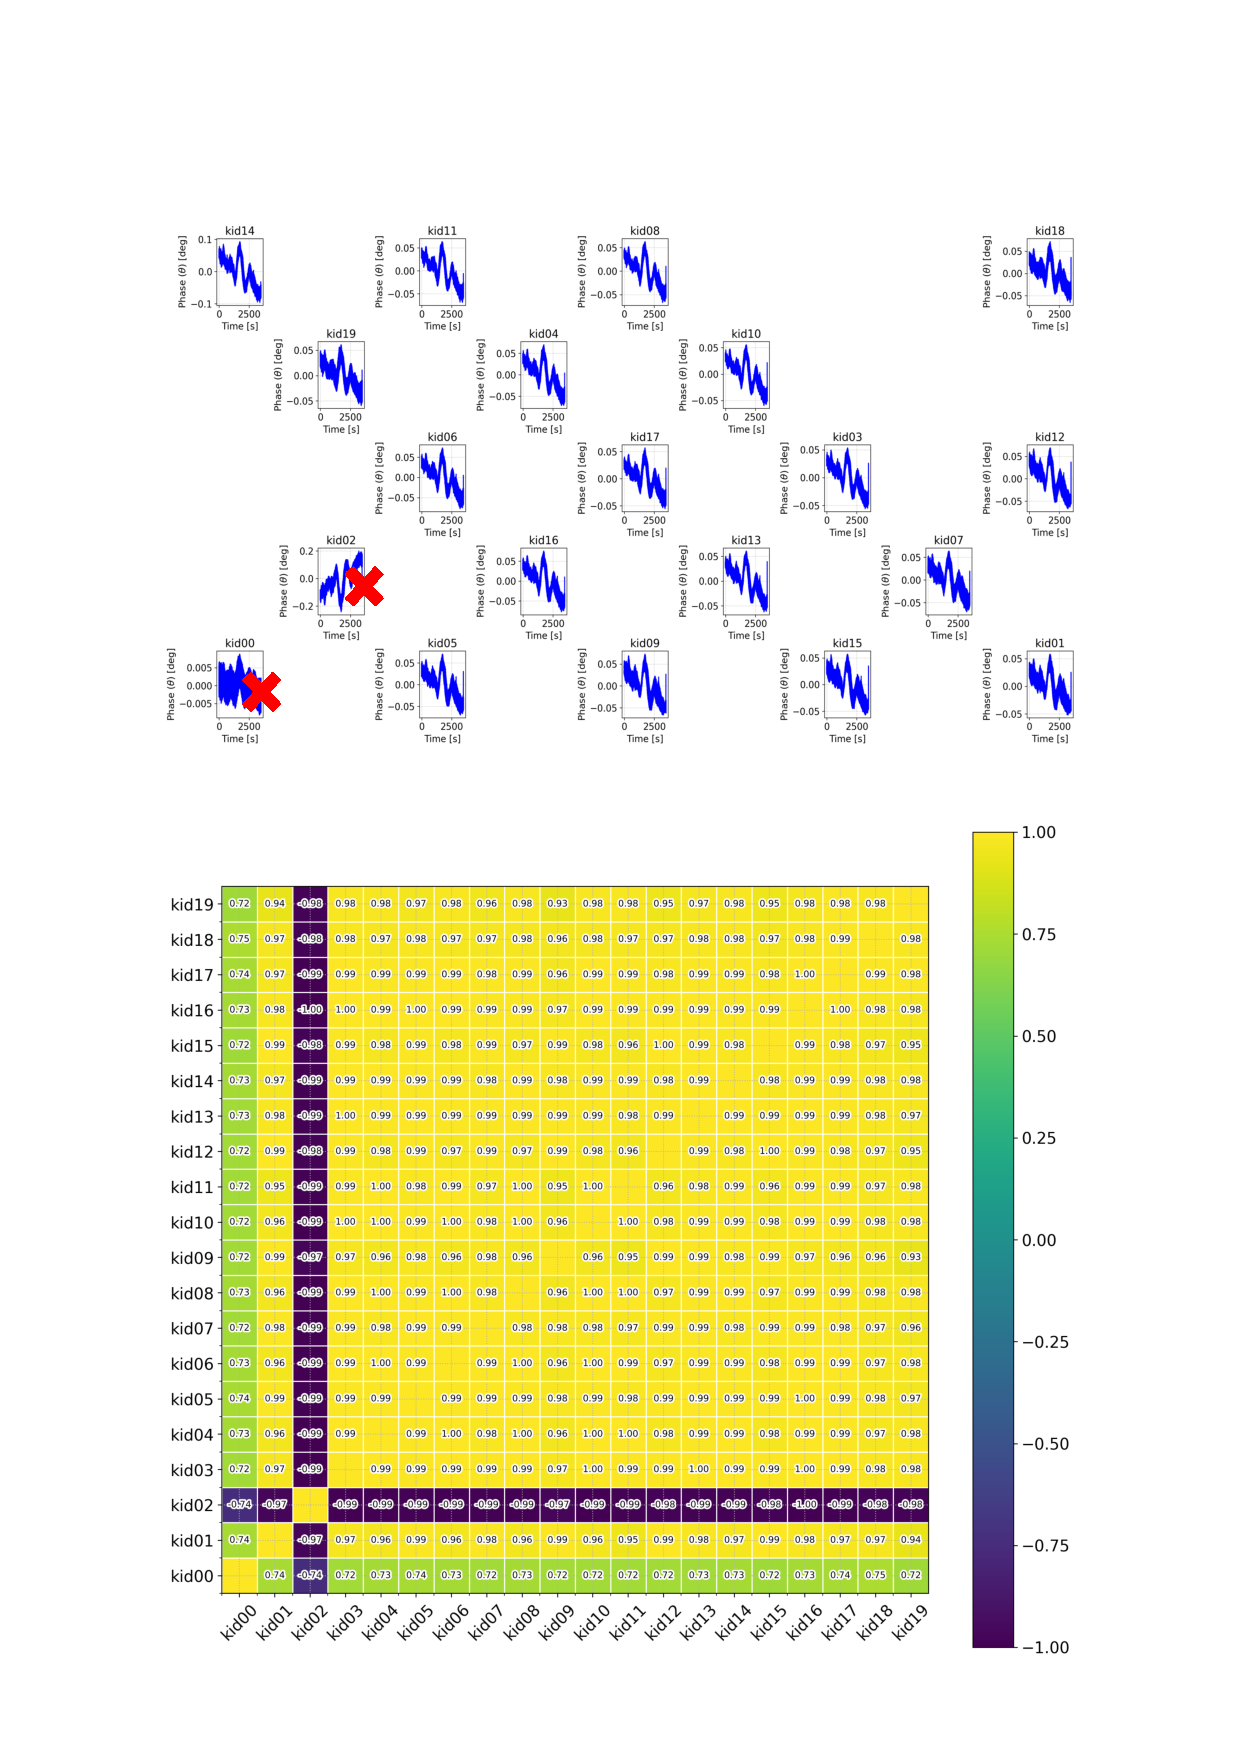
\includegraphics[width=1.0\columnwidth]{5_alignment/figs/9011_tod_cor_combined.pdf}
  \caption{hoge}
  \label{9011_tod_cor_combined}
\end{figure}
回転前TODを実際の検出器配置に沿って並べたものを図\ref{9011_tod_cor_combined}(上)に示す。TODの位相は1観測での平均値でベースラインを引いて表している。一部の検出器以外ではTODの形状が非常に似ており、共通したトレンドを持っている。異なる検出器のペアごとに求めたTODの相関係数を図\ref{9011_tod_cor_combined}(下)に示す。相関係数はピアソンの積率相関係数に従って以下の式
\begin{equation}
  r = \frac{\displaystyle\sum_{i=1}^{n}(x_{i}-\overline{x})(y_{i}-\overline{y})}{\sqrt{\displaystyle\sum_{i=1}^{n}(x_{i}-\overline{x})^{2}\displaystyle\sum_{i=1}^{n}(y_{i}-\overline{y})^{2}}}
\end{equation}
によって算出している。つまり、ここでの相関係数は同時刻での各TODについてのものである。一部の検出器(ここではkid0とkid2)を除いては相関係数は0.9を超え、強い相関を持っていることが見て取れる。このことからも、検出器間でのTODの差分を取ることで共通した大気ノイズを差し引けることを示唆している。

しかし、差分を取るにあたっては同時刻のTOD同士では不十分である。各検出器で同時刻に見ている空は異なっており、厳密な相関を見るためには理想的に同じ空をスキャンした時刻のTOD同士で差分を取る必要がある。そのため、TOD間でスキャンに伴う時間差(本論文ではtiming offsetと呼ぶ)を考慮して差分をとる。2つのTOD($\mathrm{TOD}_{1}$, $\mathrm{TOD}_{2}$)の差分をとったTOD($\mathrm{TOD}_{diff}$)は

\subsection{timing offsetの算出}

\subsection{PSDと自己相関}

\subsection{大気揺らぎ抑制の確認}
